\chapter{Scan Data Hadronic Counting Fits}
\label{app:nonDDbar_hadron_counts_scan}

\begin{figure}[H]
\centering
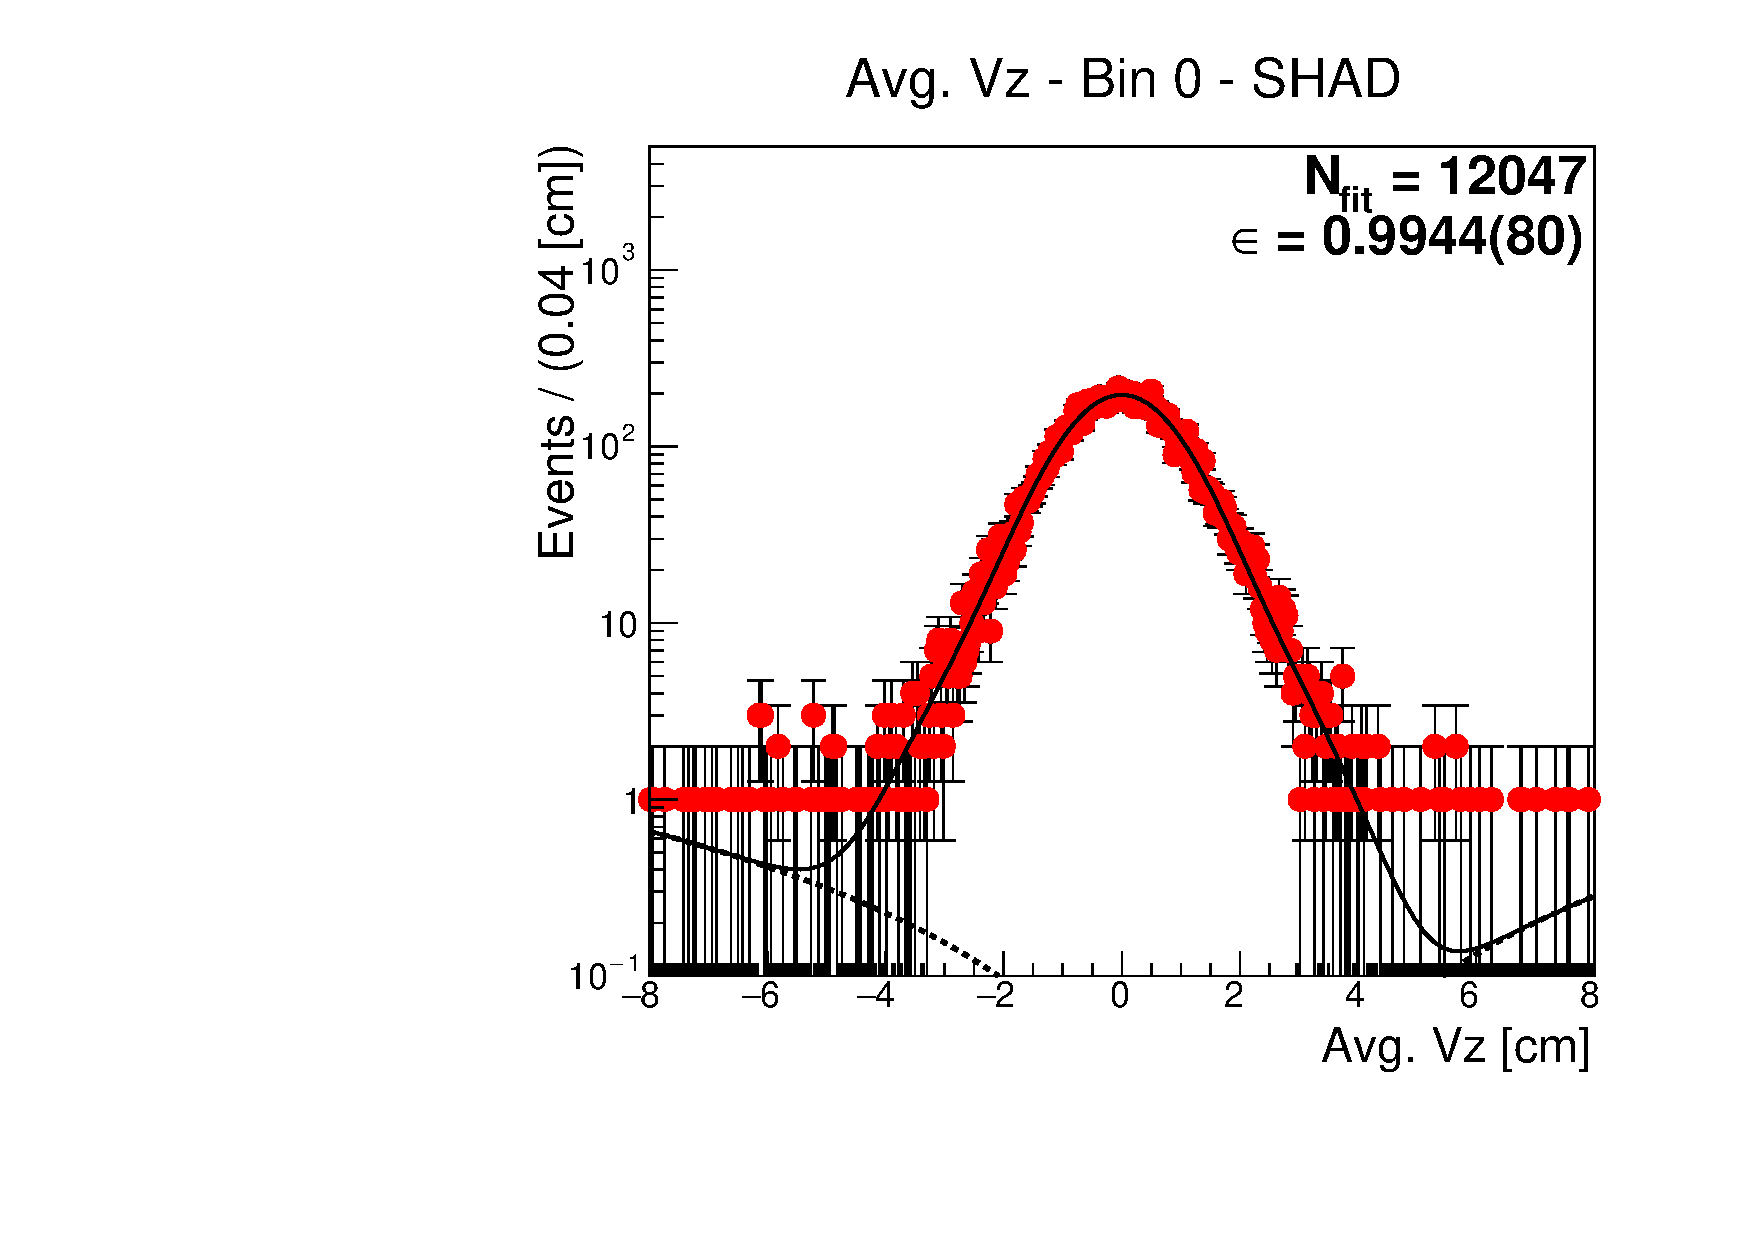
\includegraphics[scale=0.25]{figures/plots/nonDDbar_fit_results/scan/fit_scan_00_data_SHAD.pdf}
\hspace{-0.5cm}
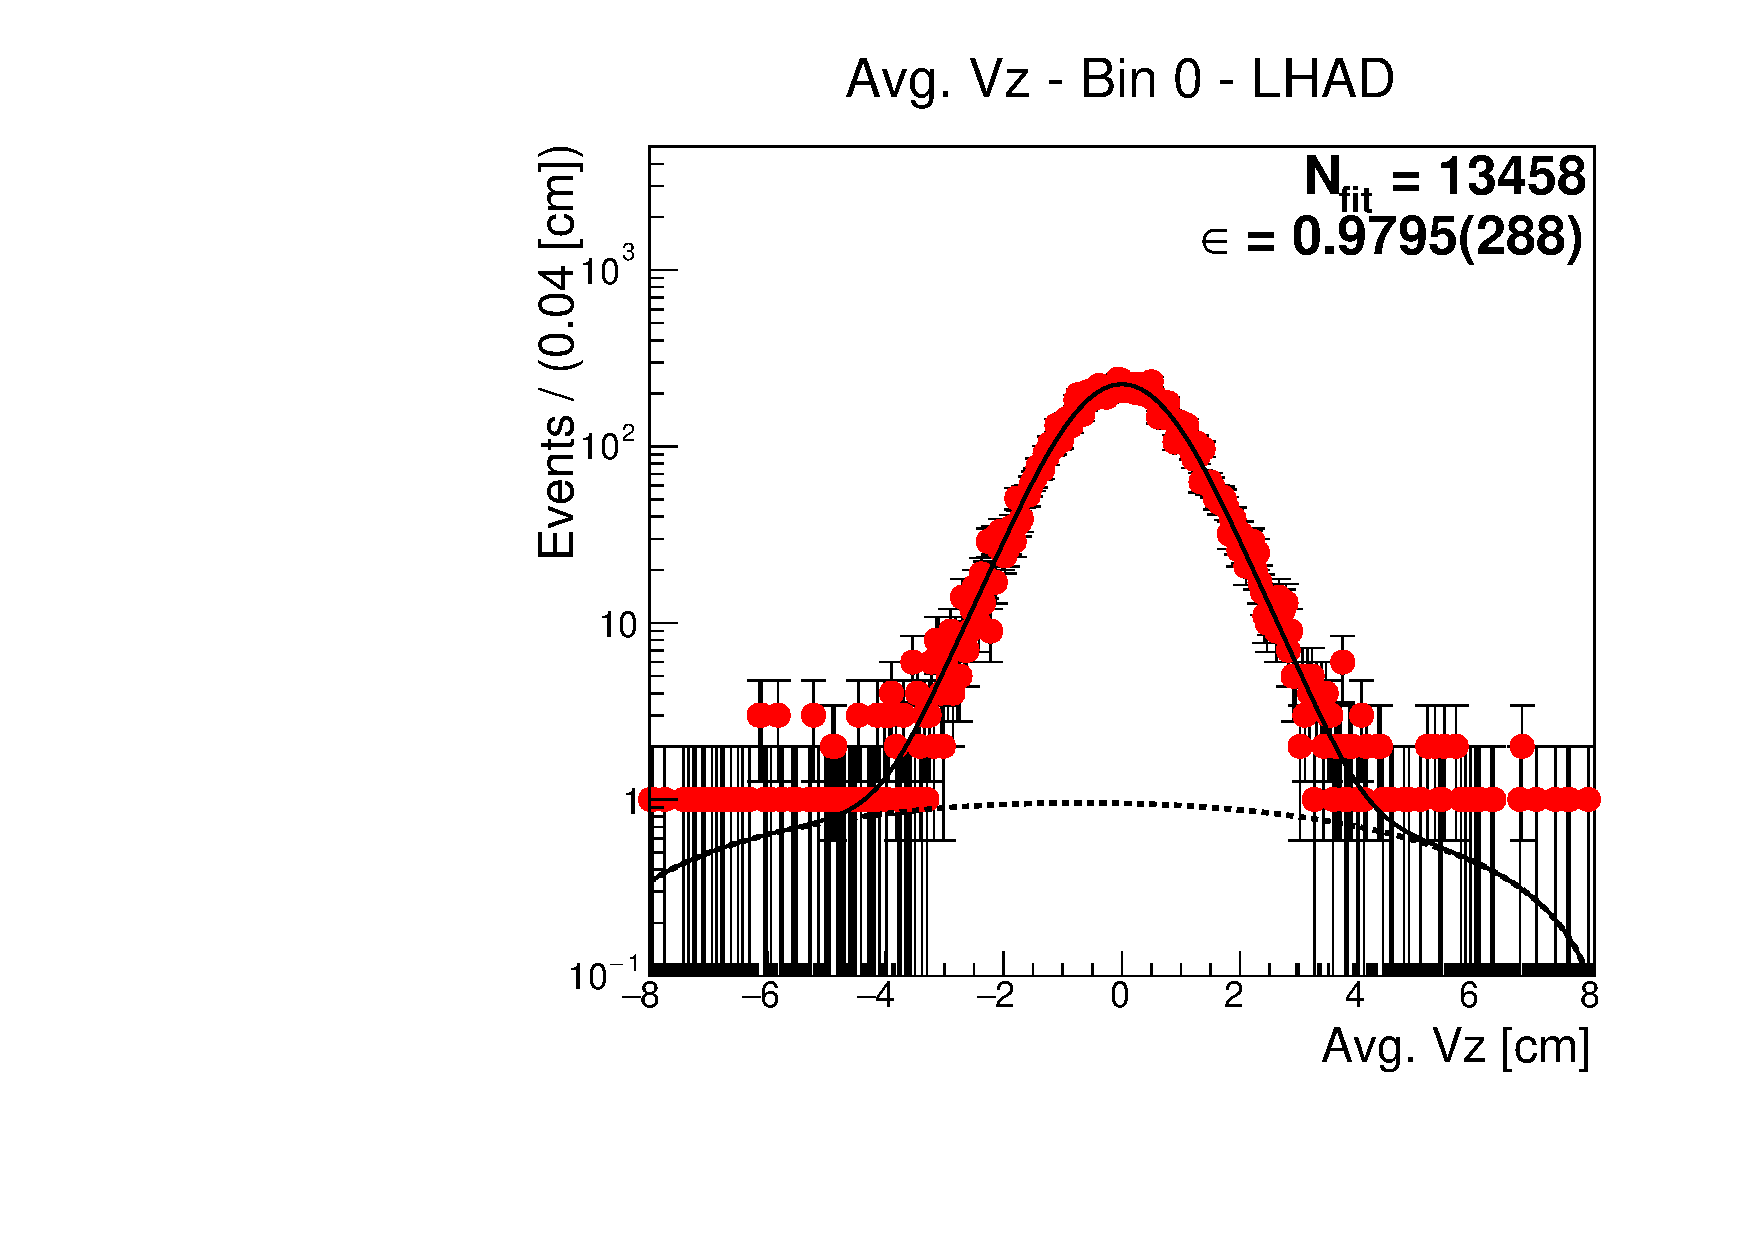
\includegraphics[scale=0.25]{figures/plots/nonDDbar_fit_results/scan/fit_scan_00_data_LHAD.pdf}
\hspace{-0.5cm}
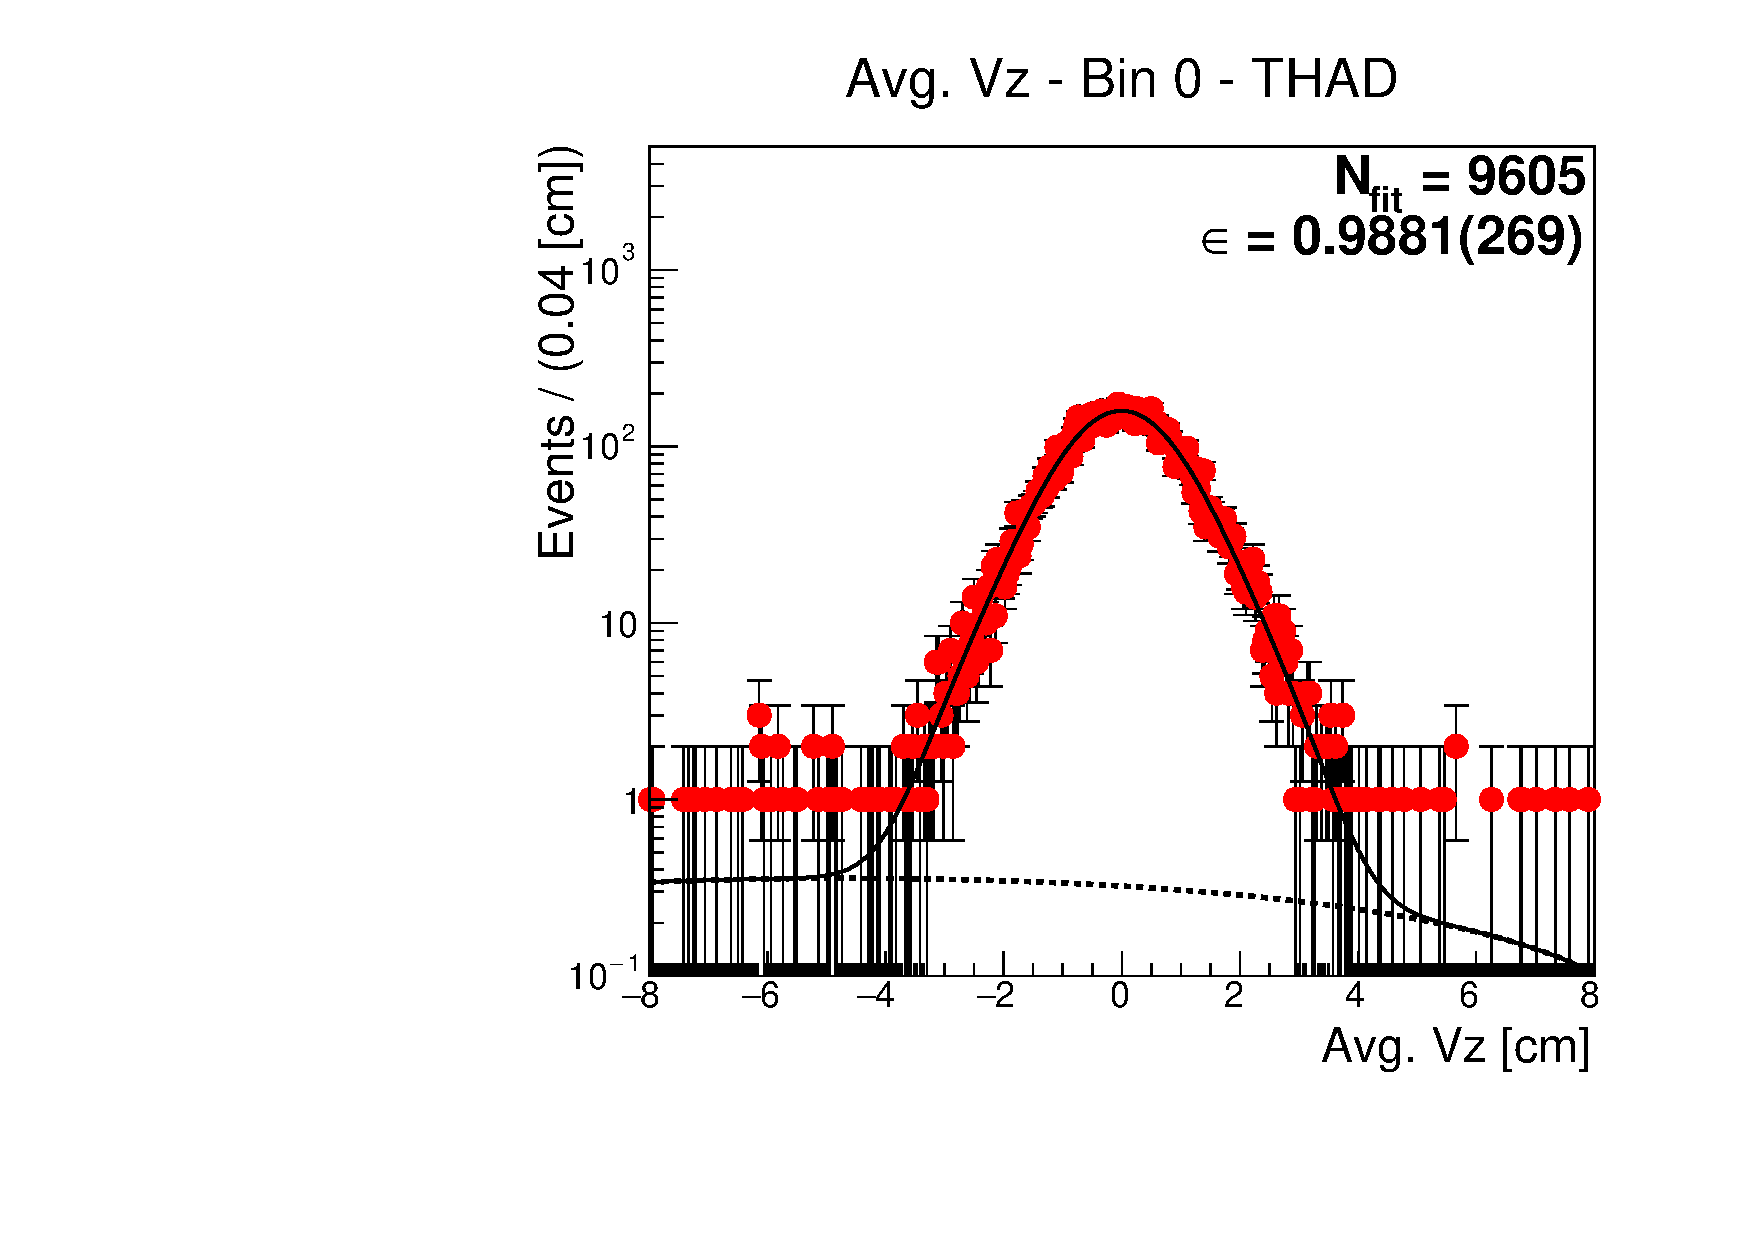
\includegraphics[scale=0.25]{figures/plots/nonDDbar_fit_results/scan/fit_scan_00_data_THAD.pdf}
\caption{Fits to determine the number of hadrons in the 3734 (Scan) data sample.}
{This includes results for SHAD (left), LHAD (middle), and THAD (right).}
\label{fig:hadron_fits_scan_00}
\end{figure}

\begin{figure}[H]
\centering
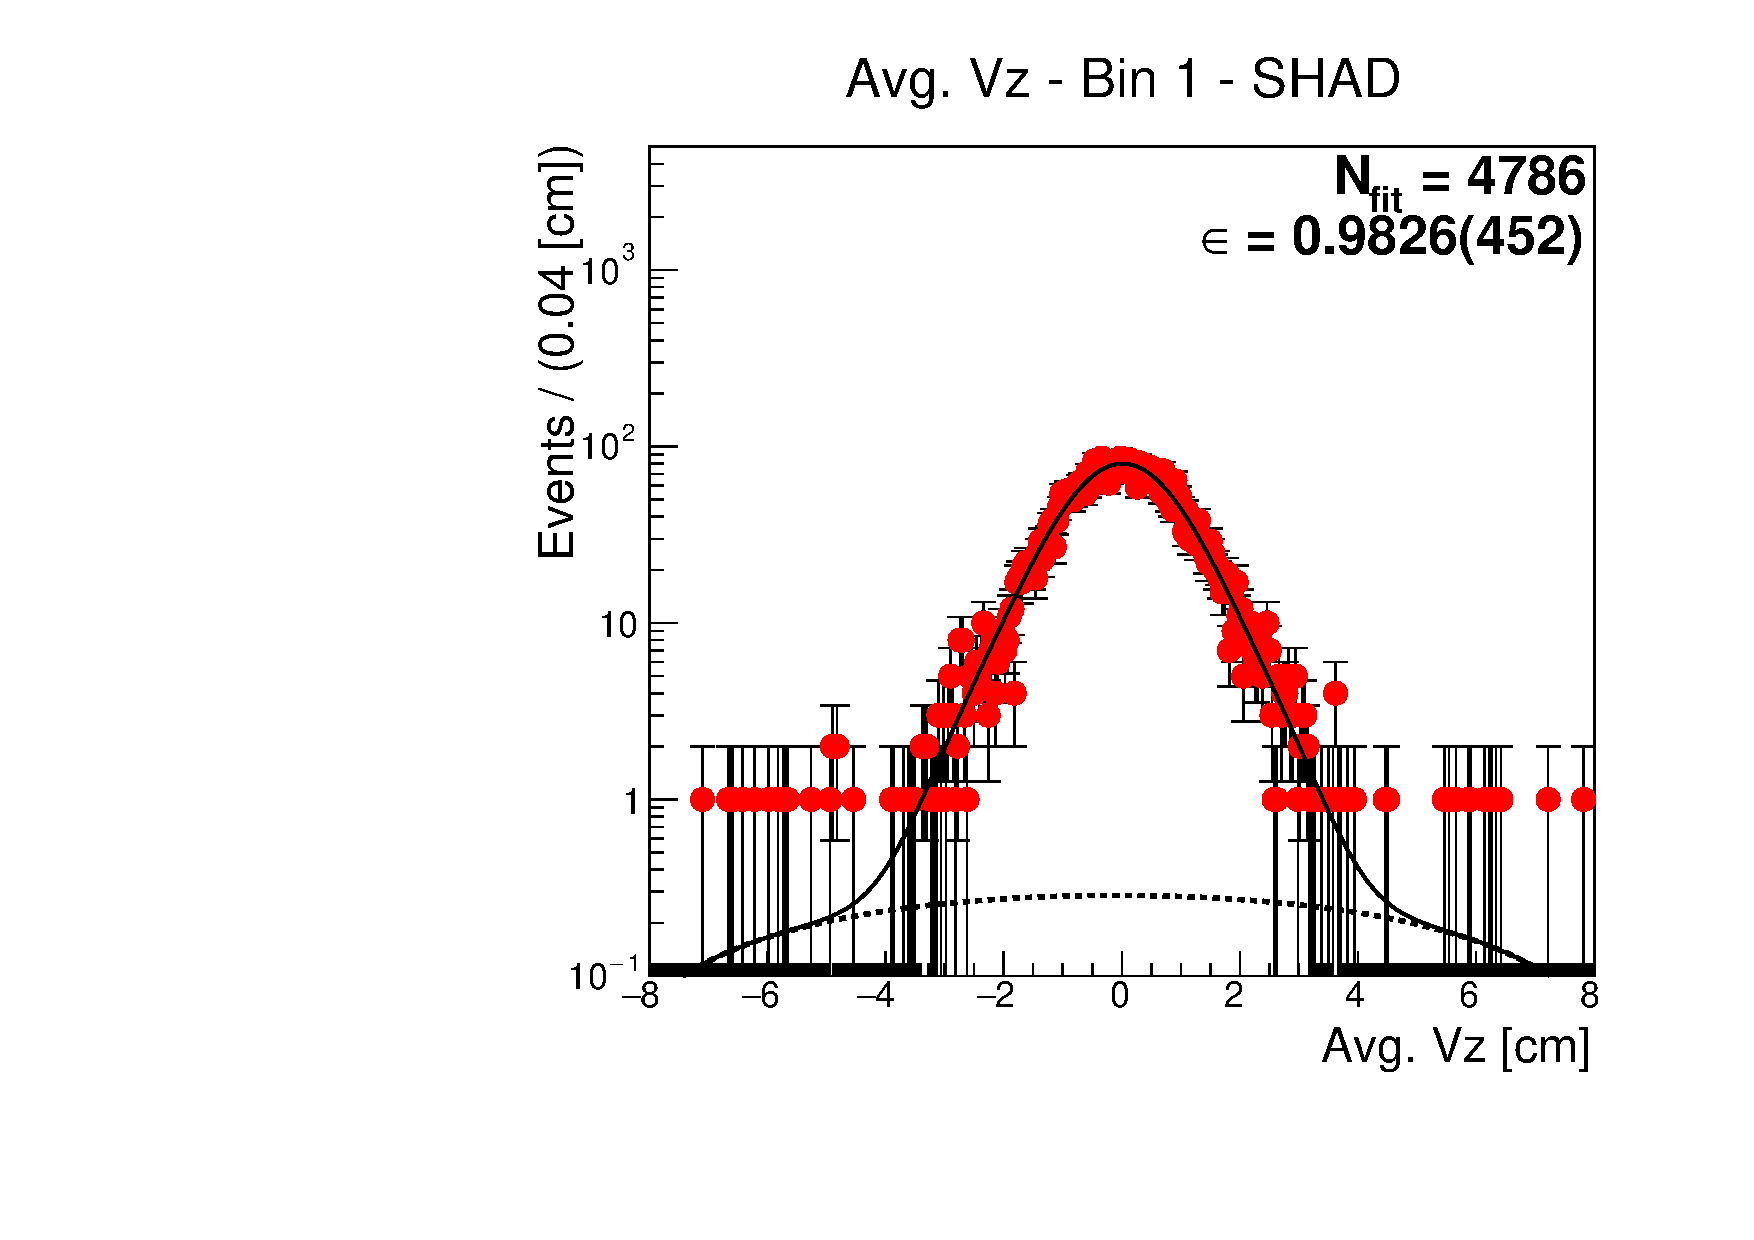
\includegraphics[scale=0.25]{figures/plots/nonDDbar_fit_results/scan/fit_scan_01_data_SHAD.pdf}
\hspace{-0.5cm}
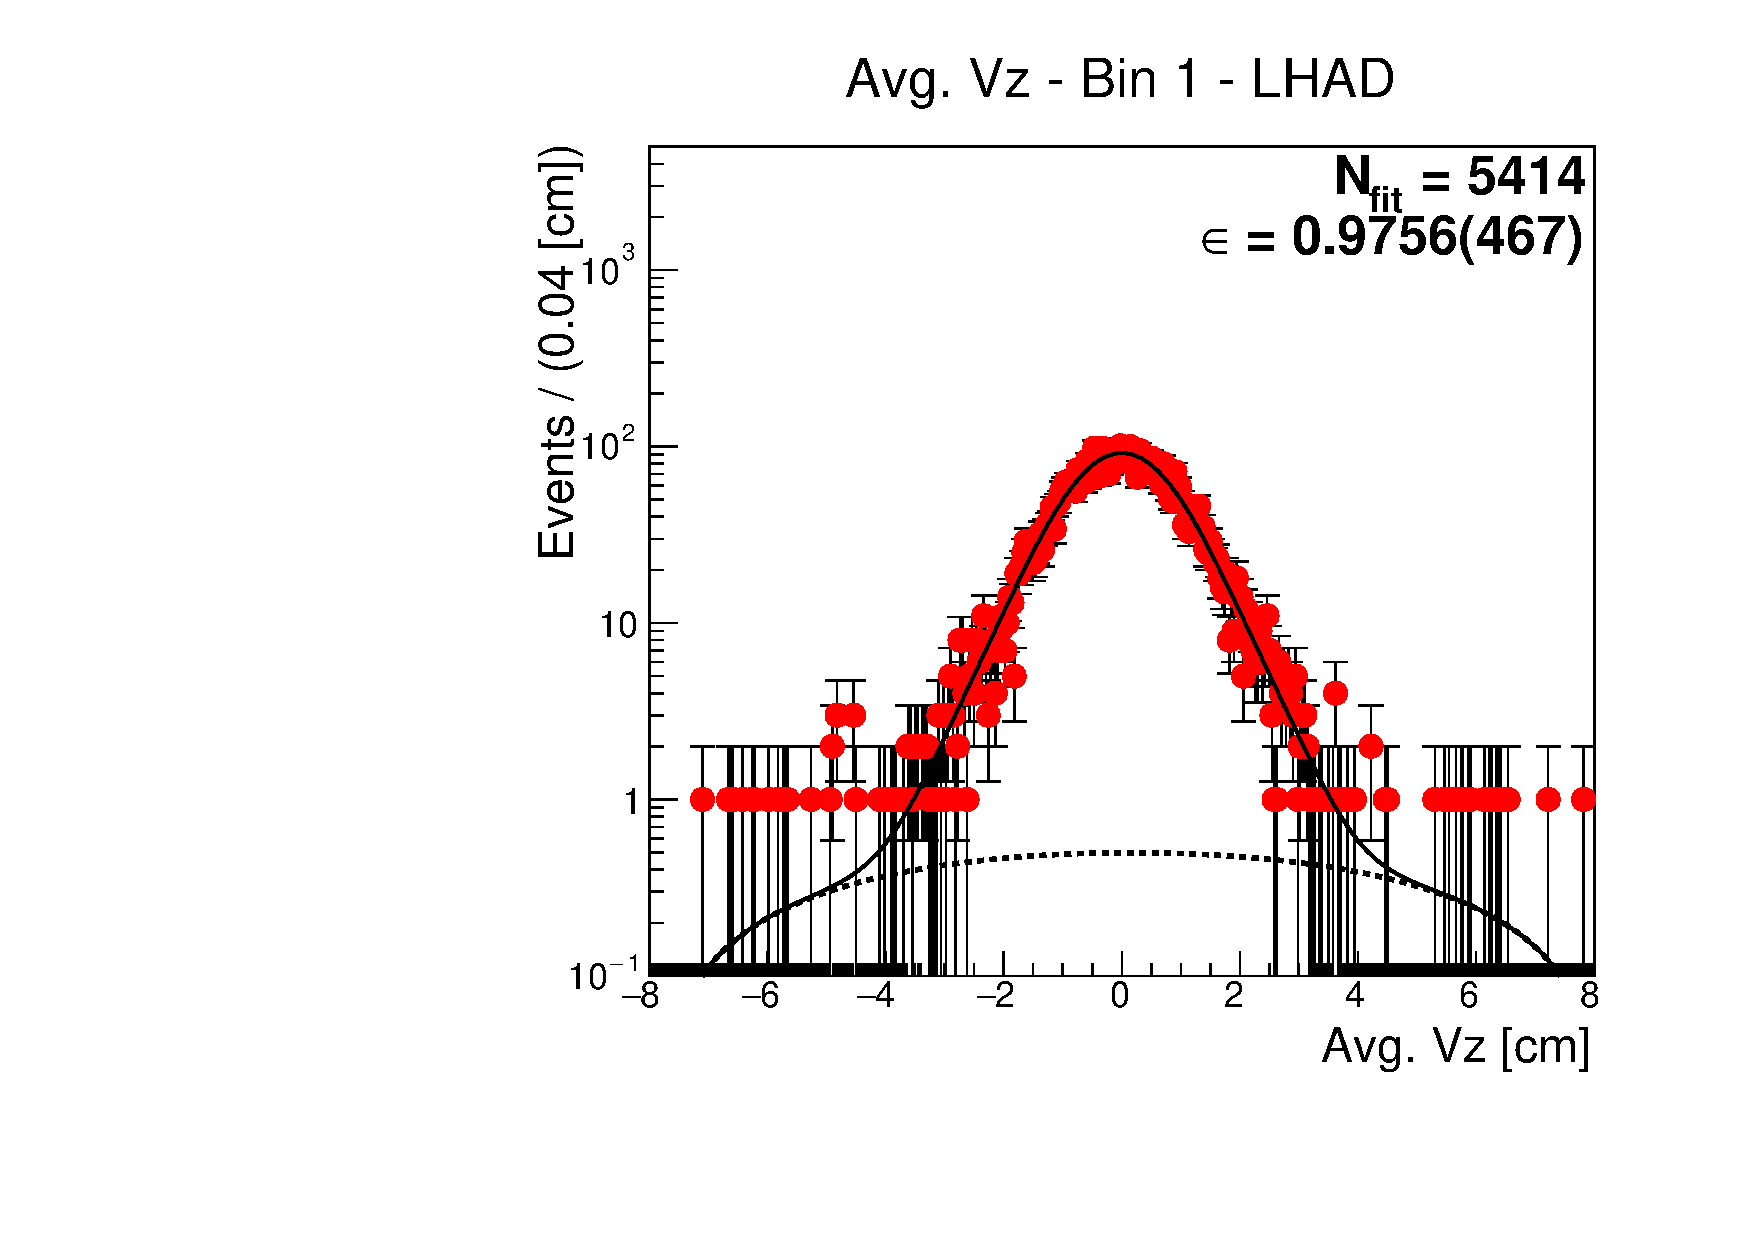
\includegraphics[scale=0.25]{figures/plots/nonDDbar_fit_results/scan/fit_scan_01_data_LHAD.pdf}
\hspace{-0.5cm}
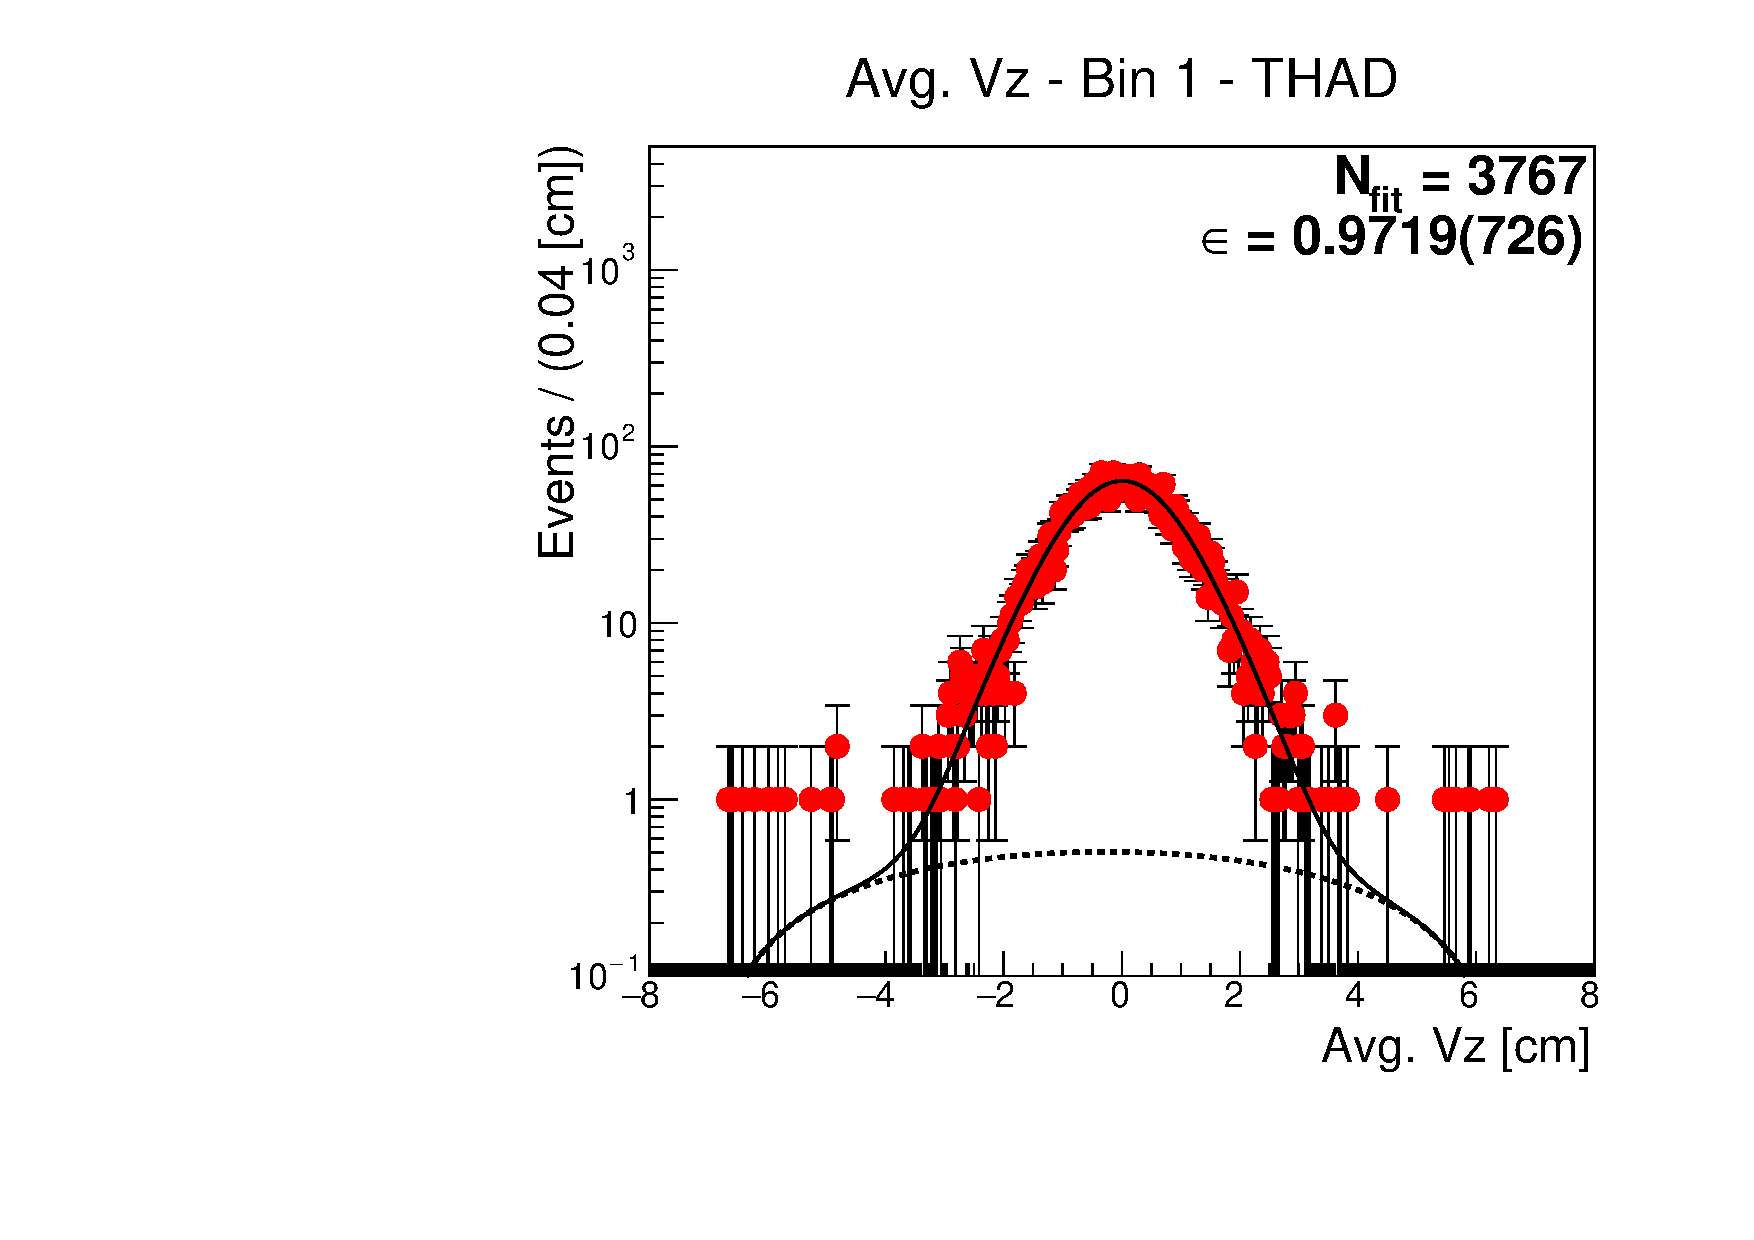
\includegraphics[scale=0.25]{figures/plots/nonDDbar_fit_results/scan/fit_scan_01_data_THAD.pdf}
\caption{Fits to determine the number of hadrons in the 3736 (Scan) data sample.}
{This includes results for SHAD (left), LHAD (middle), and THAD (right).}
\label{fig:hadron_fits_scan_01}
\end{figure}

\begin{figure}[H]
\centering
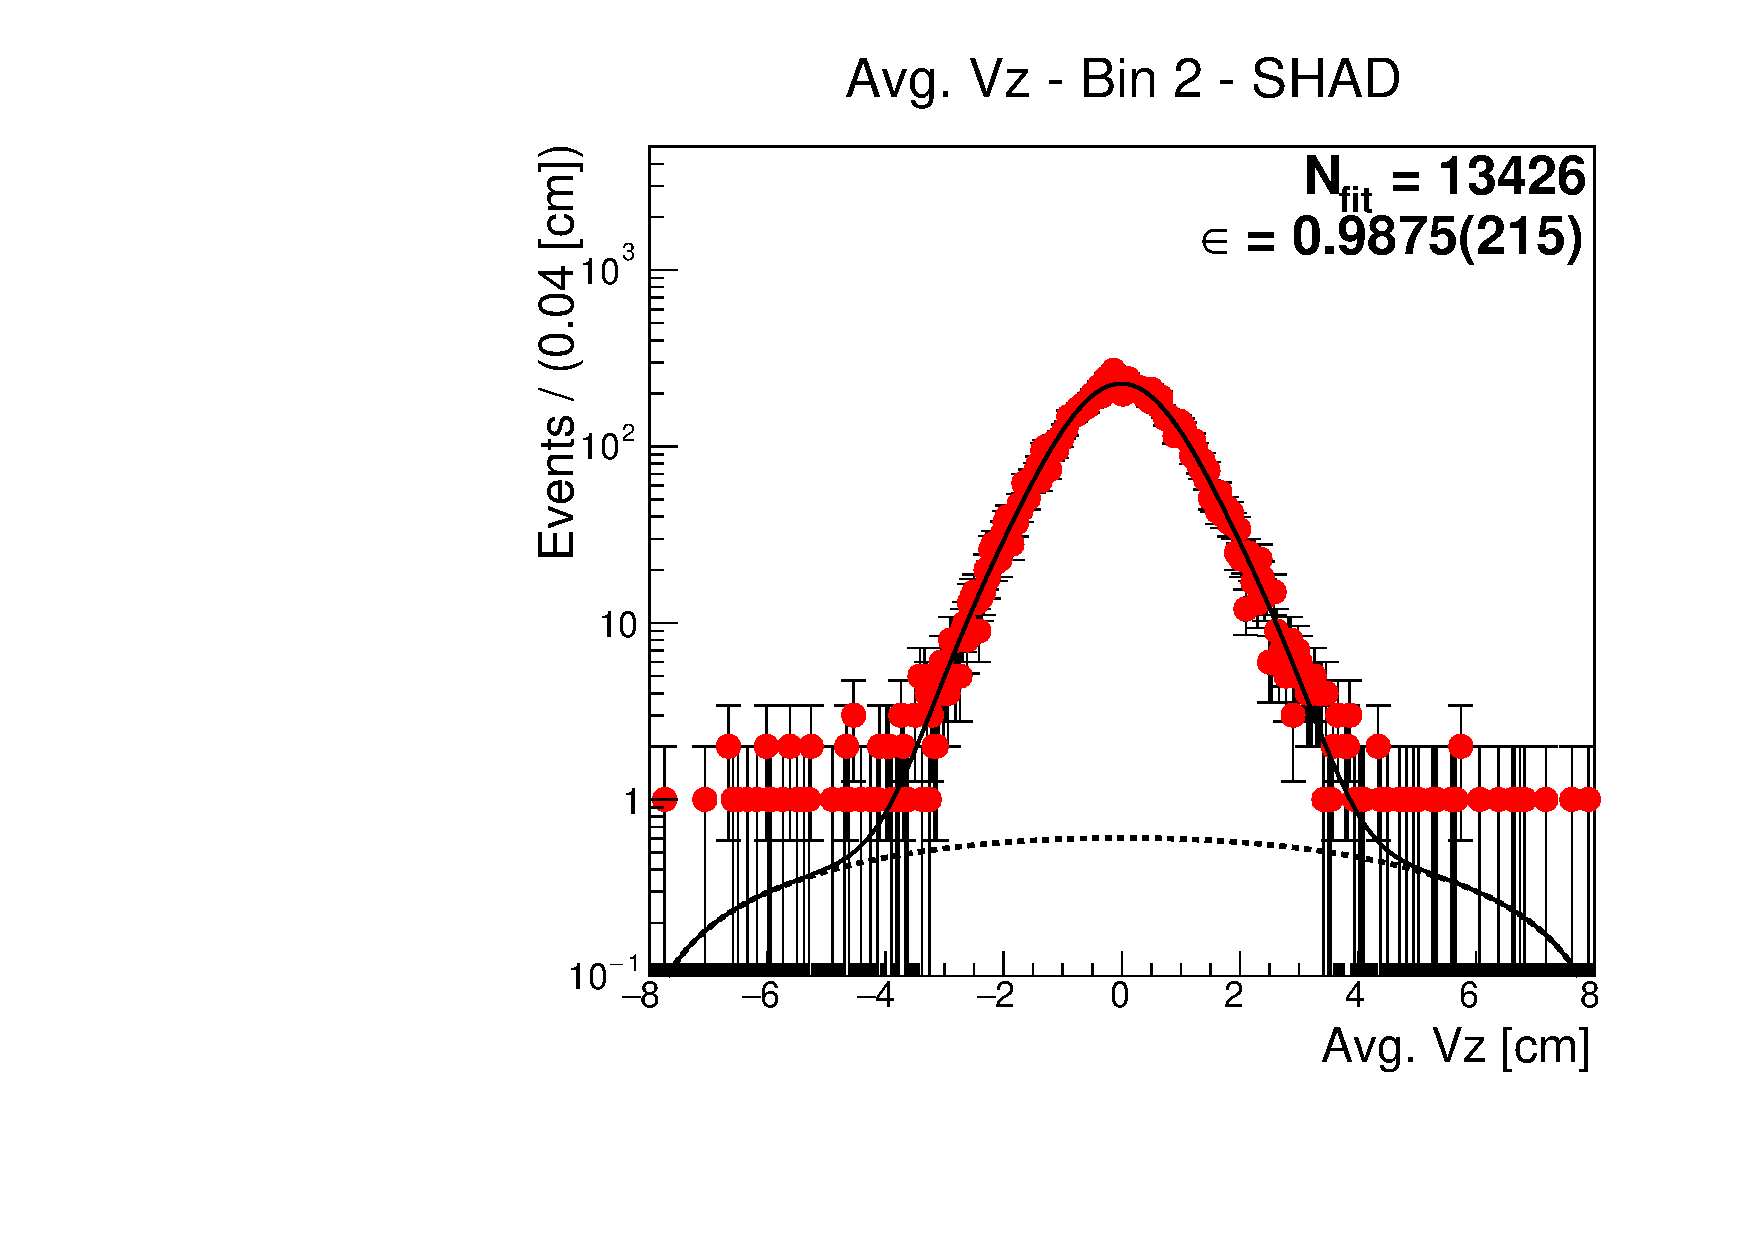
\includegraphics[scale=0.25]{figures/plots/nonDDbar_fit_results/scan/fit_scan_02_data_SHAD.pdf}
\hspace{-0.5cm}
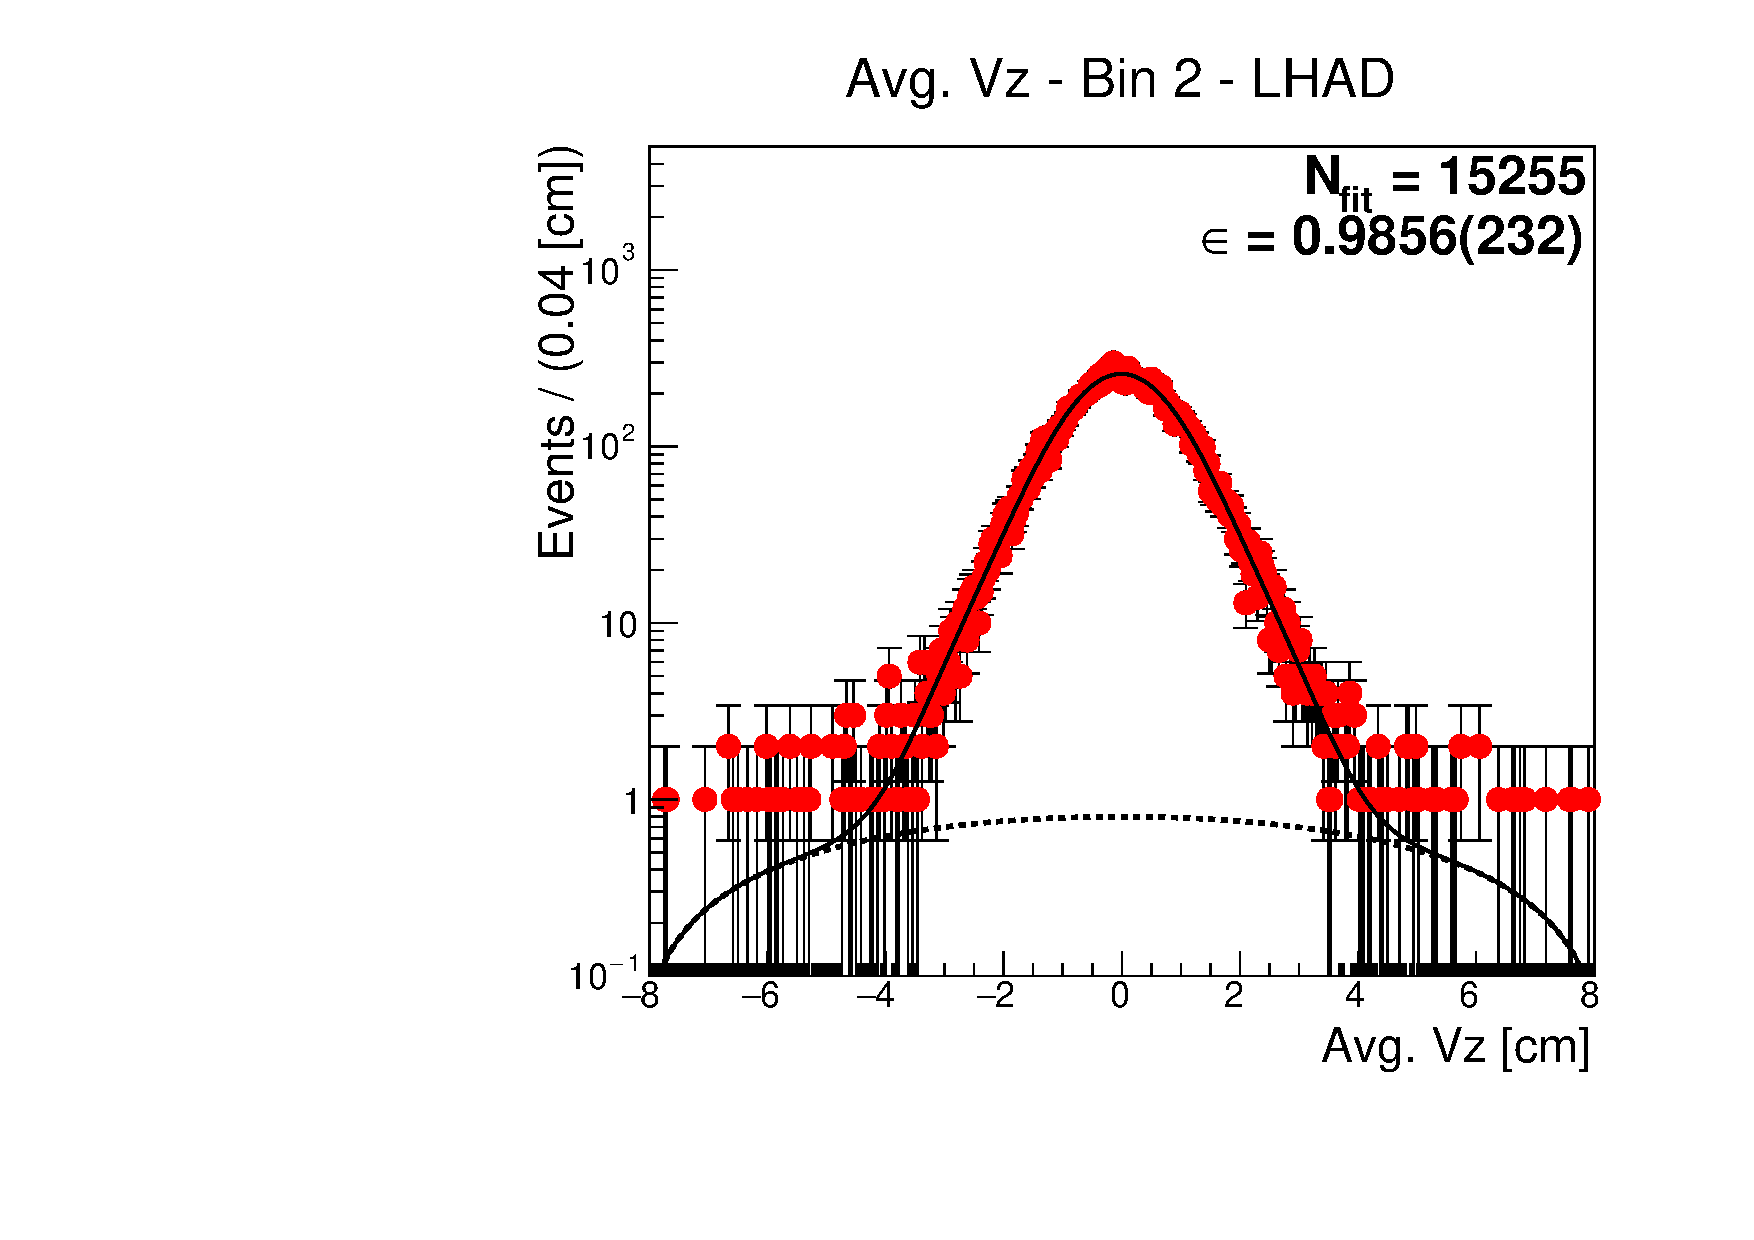
\includegraphics[scale=0.25]{figures/plots/nonDDbar_fit_results/scan/fit_scan_02_data_LHAD.pdf}
\hspace{-0.5cm}
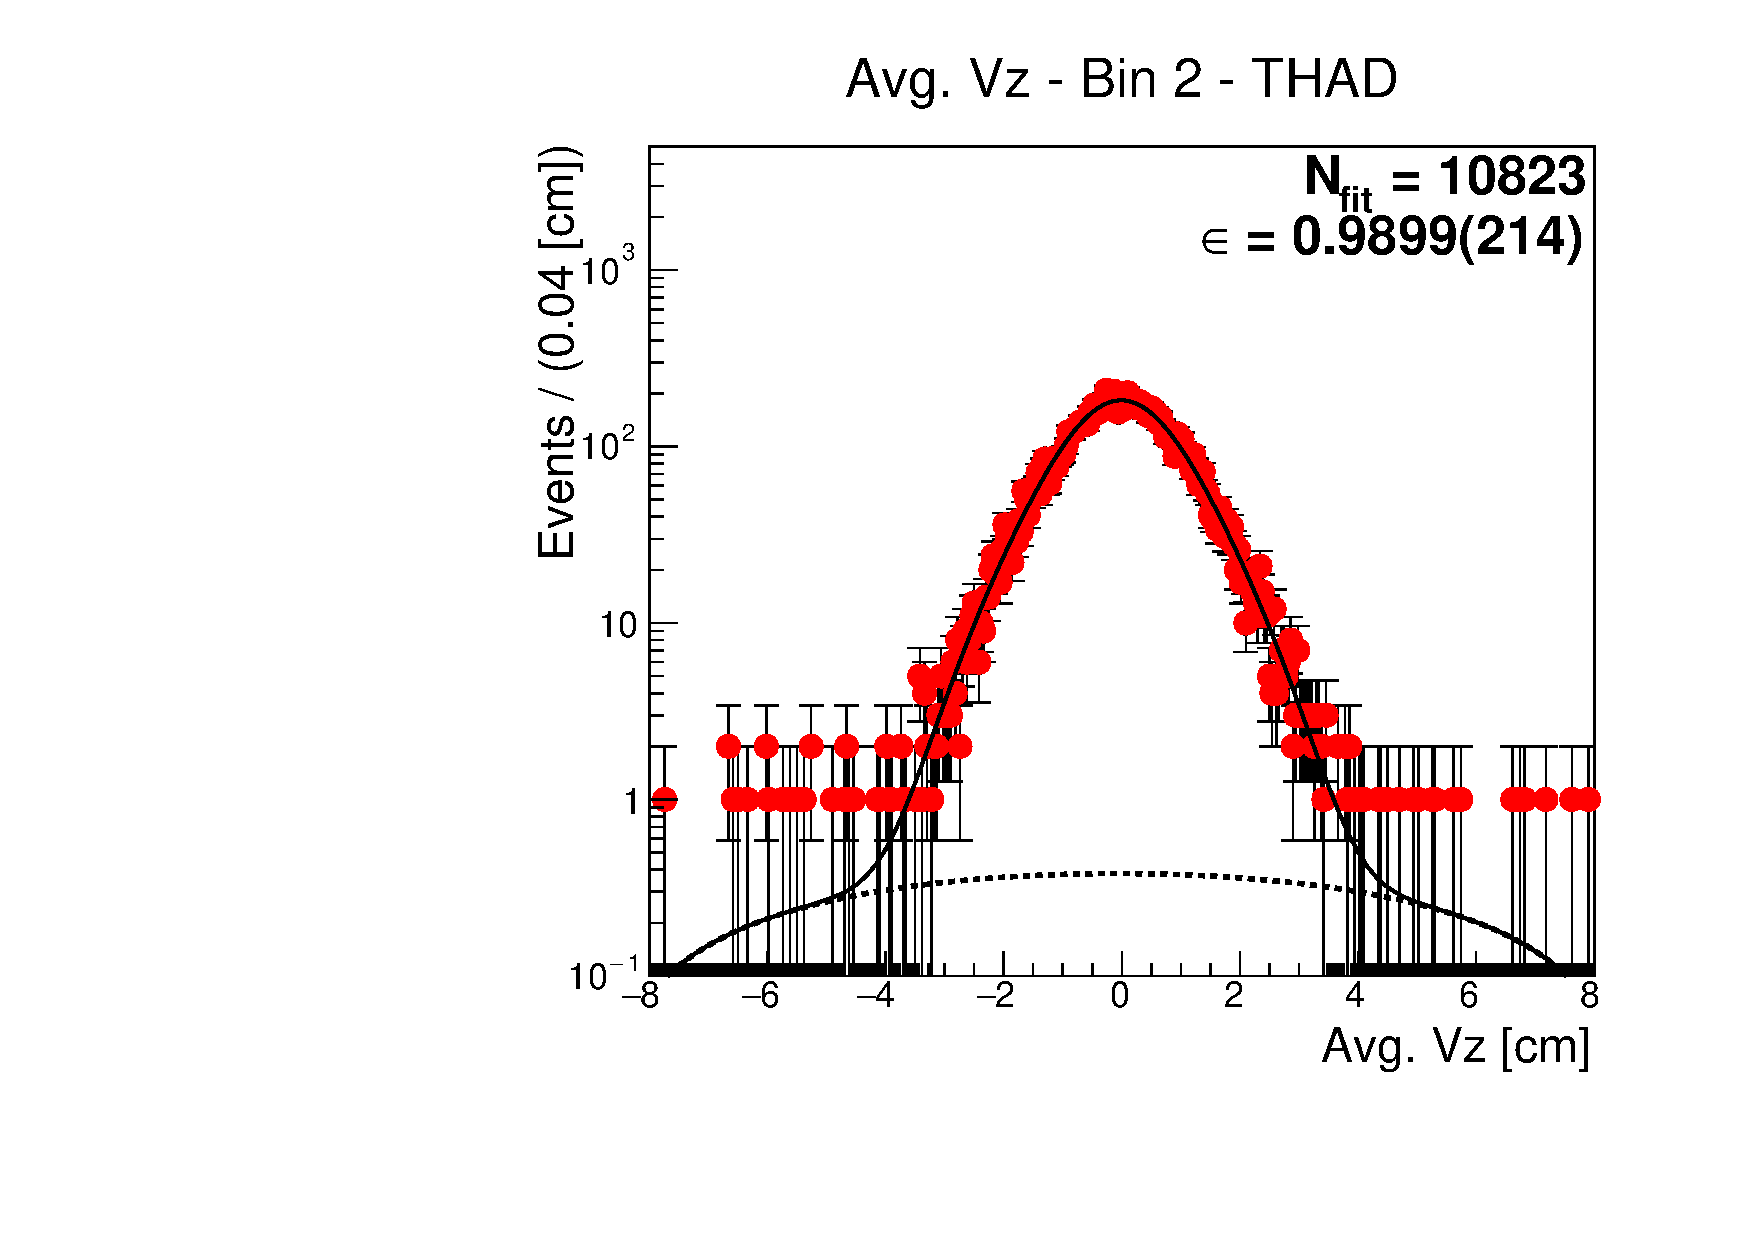
\includegraphics[scale=0.25]{figures/plots/nonDDbar_fit_results/scan/fit_scan_02_data_THAD.pdf}
\caption{Fits to determine the number of hadrons in the 3744 (Scan) data sample.}
{This includes results for SHAD (left), LHAD (middle), and THAD (right).}
\label{fig:hadron_fits_scan_02}
\end{figure}

\begin{figure}[H]
\centering
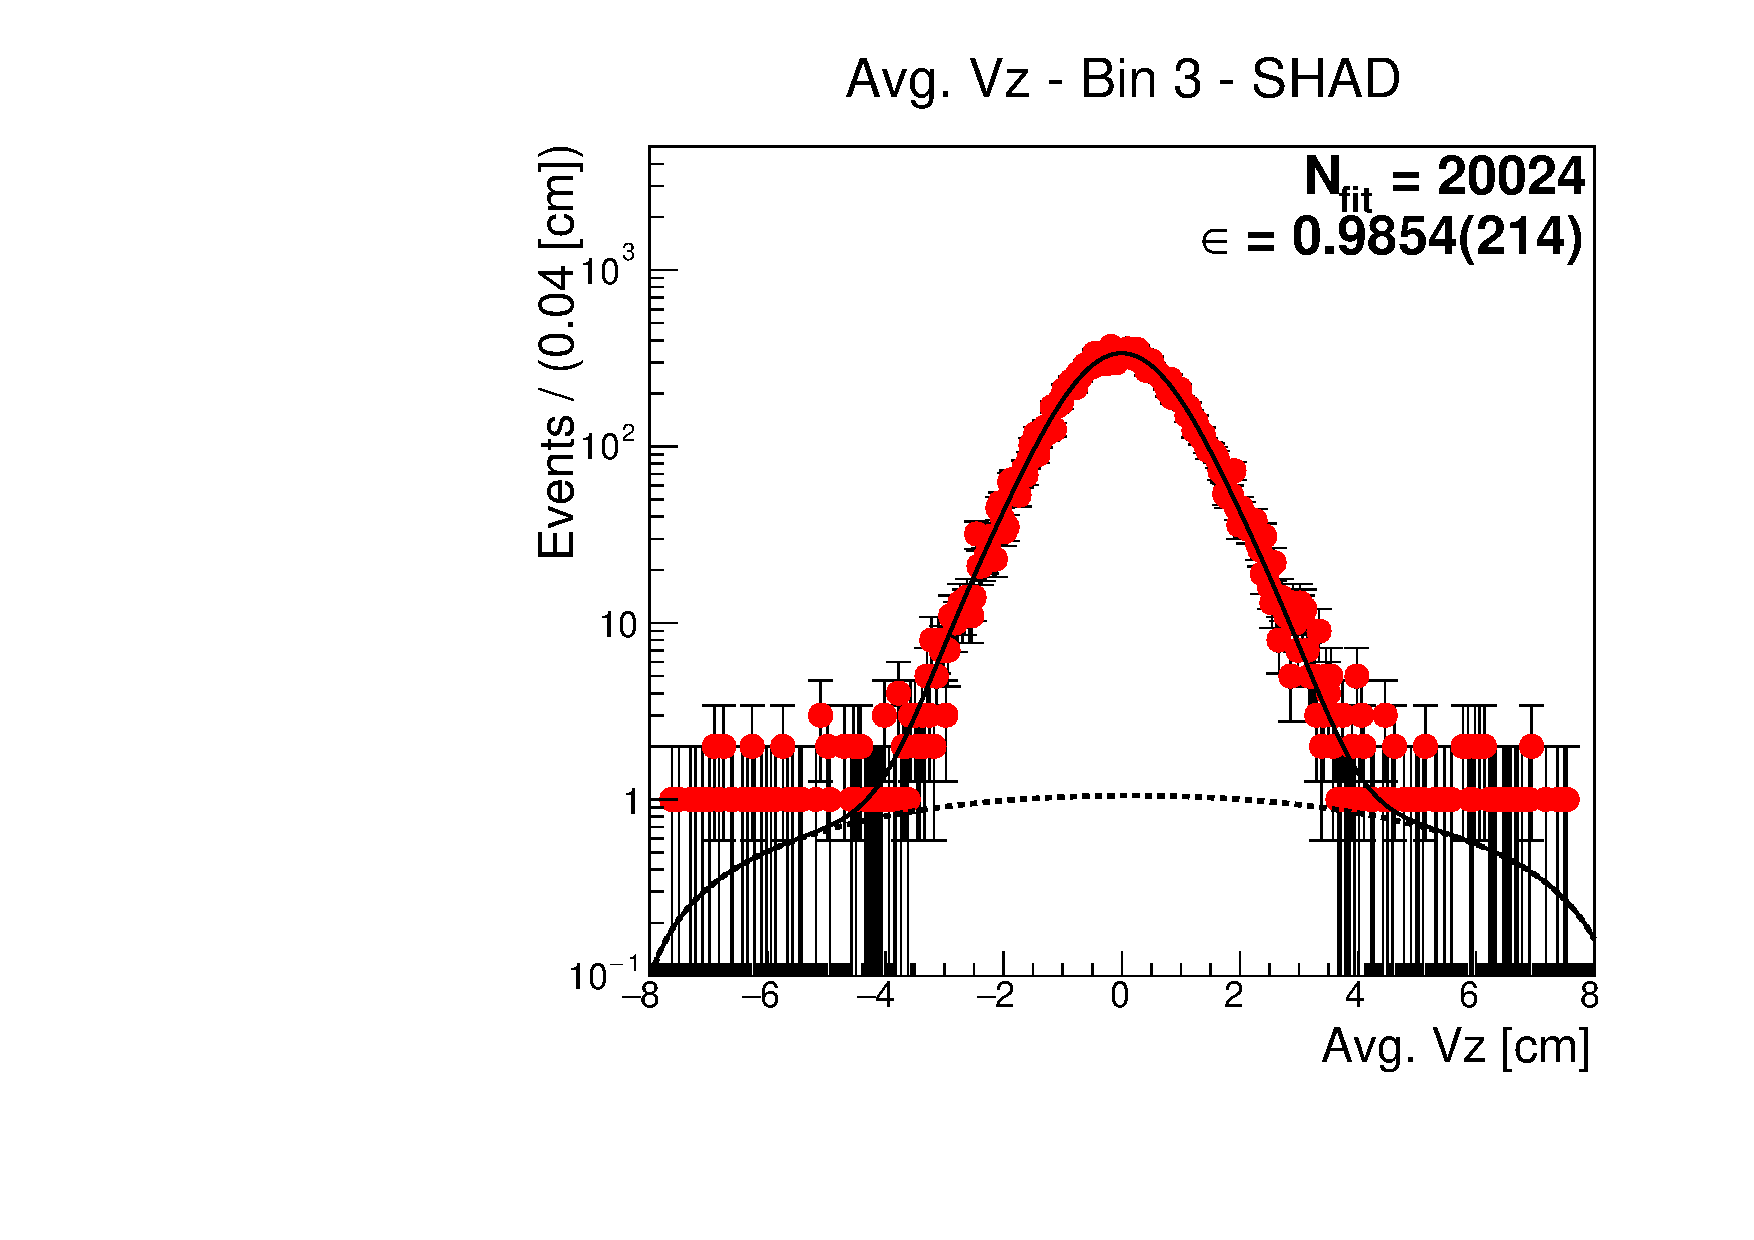
\includegraphics[scale=0.25]{figures/plots/nonDDbar_fit_results/scan/fit_scan_03_data_SHAD.pdf}
\hspace{-0.5cm}
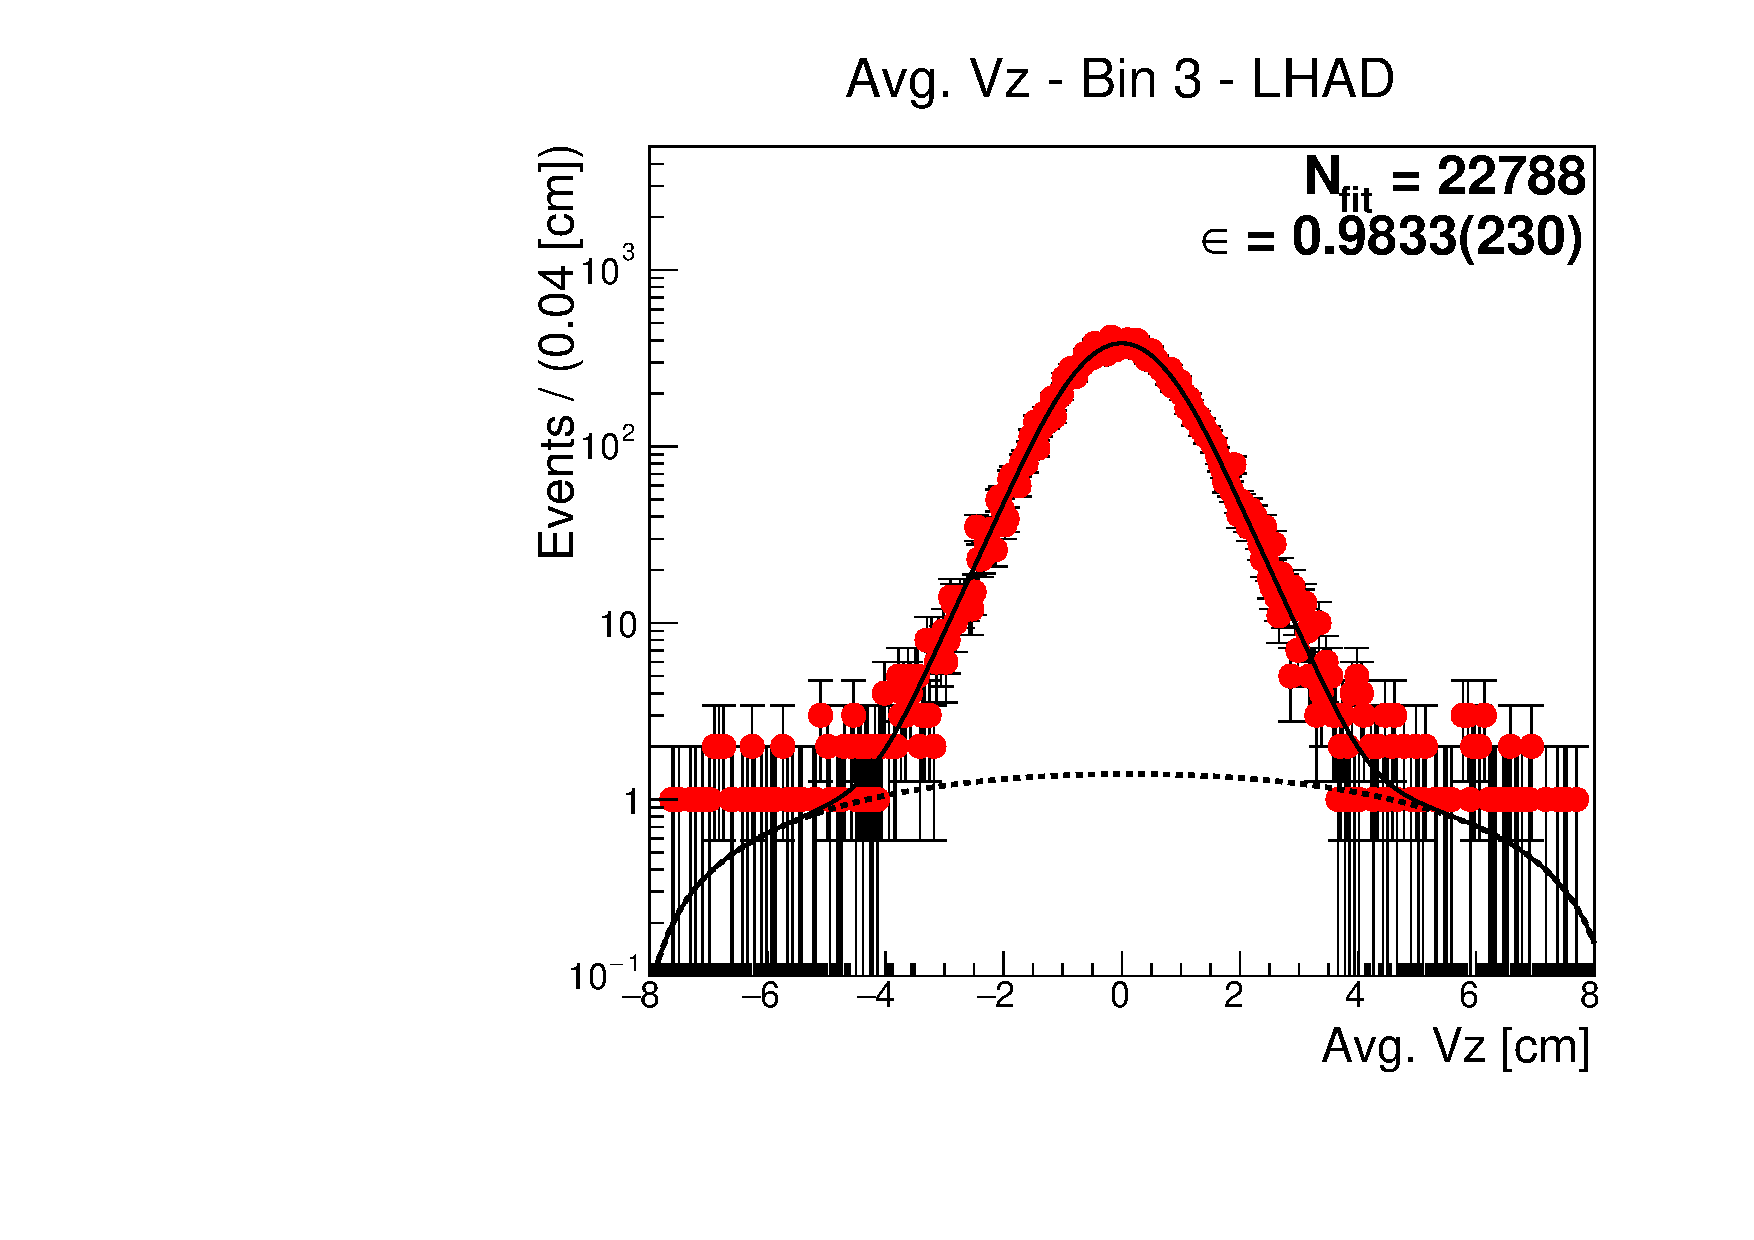
\includegraphics[scale=0.25]{figures/plots/nonDDbar_fit_results/scan/fit_scan_03_data_LHAD.pdf}
\hspace{-0.5cm}
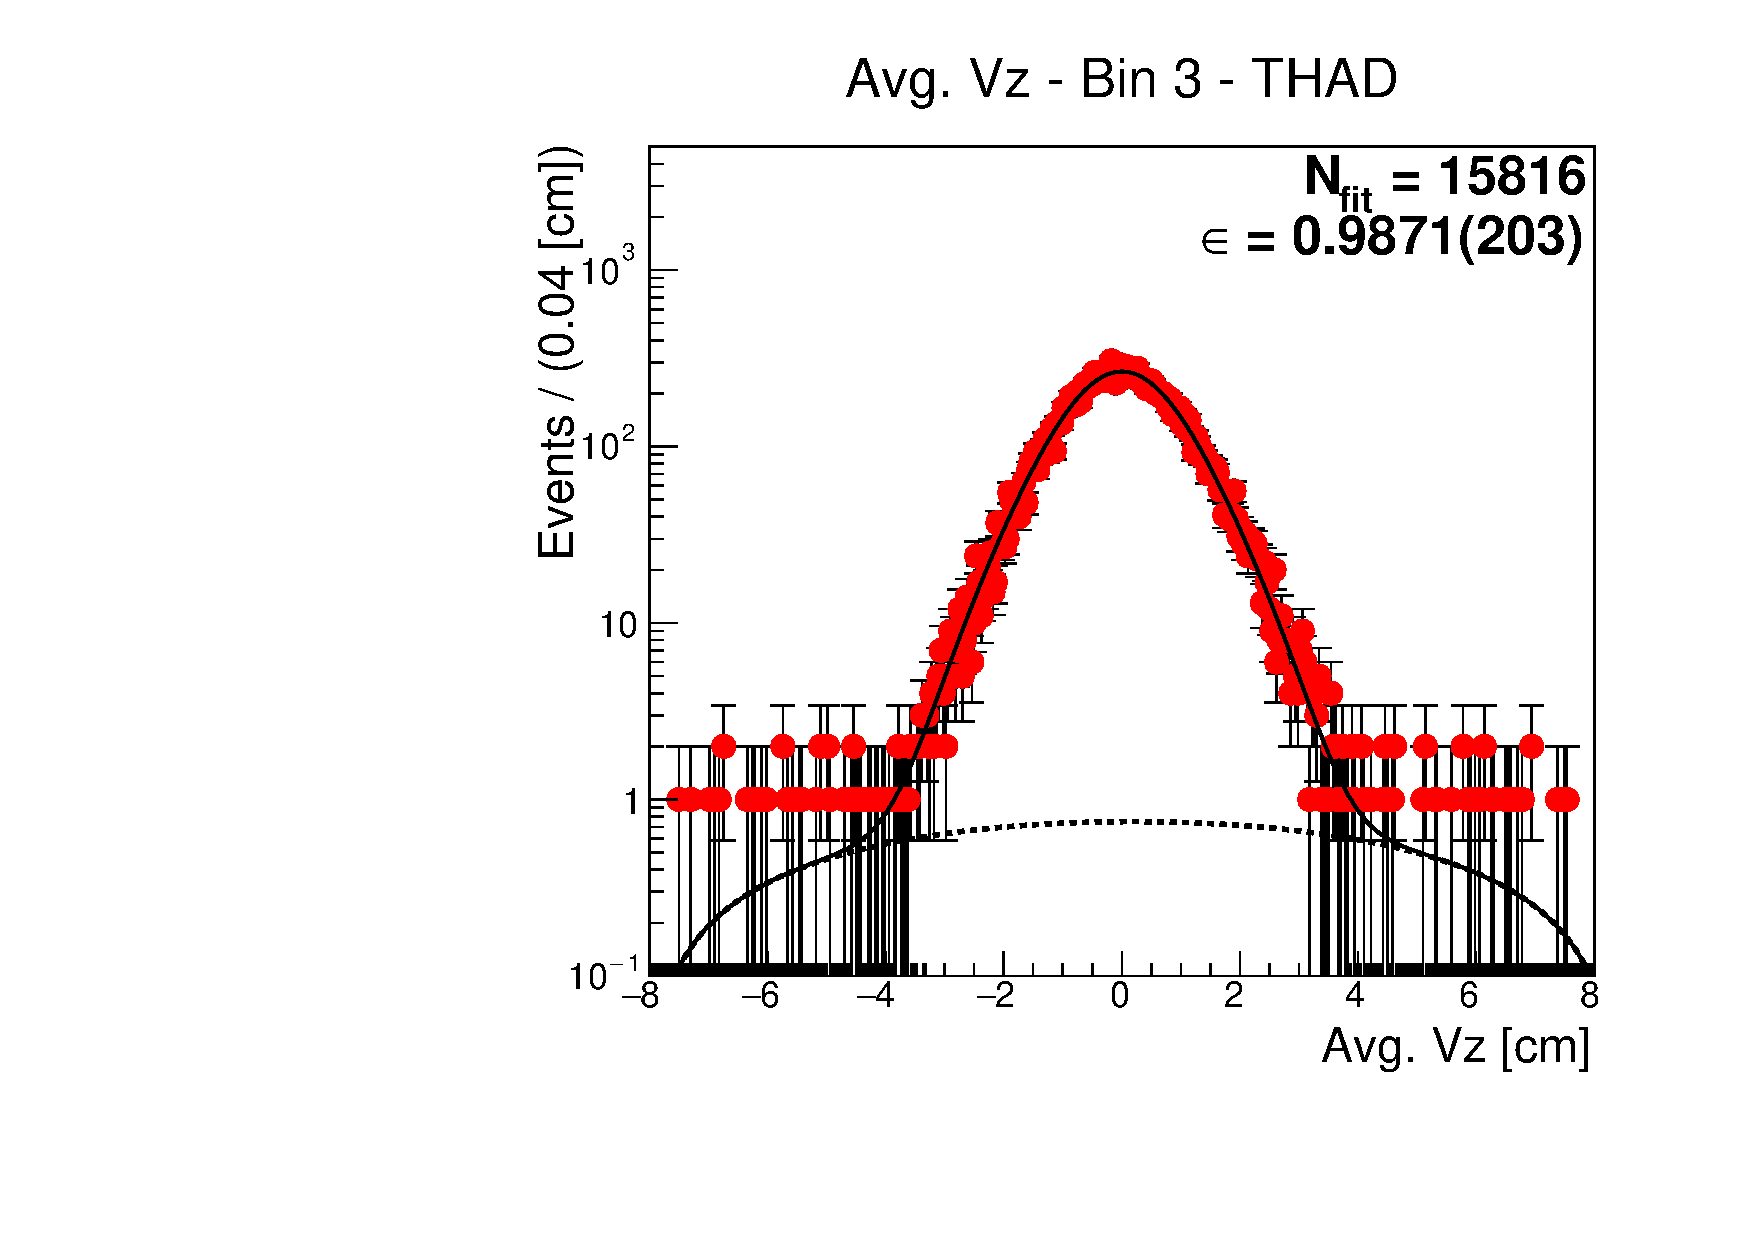
\includegraphics[scale=0.25]{figures/plots/nonDDbar_fit_results/scan/fit_scan_03_data_THAD.pdf}
\caption{Fits to determine the number of hadrons in the 3748 (Scan) data sample.}
{This includes results for SHAD (left), LHAD (middle), and THAD (right).}
\label{fig:hadron_fits_scan_03}
\end{figure}

\begin{figure}[H]
\centering
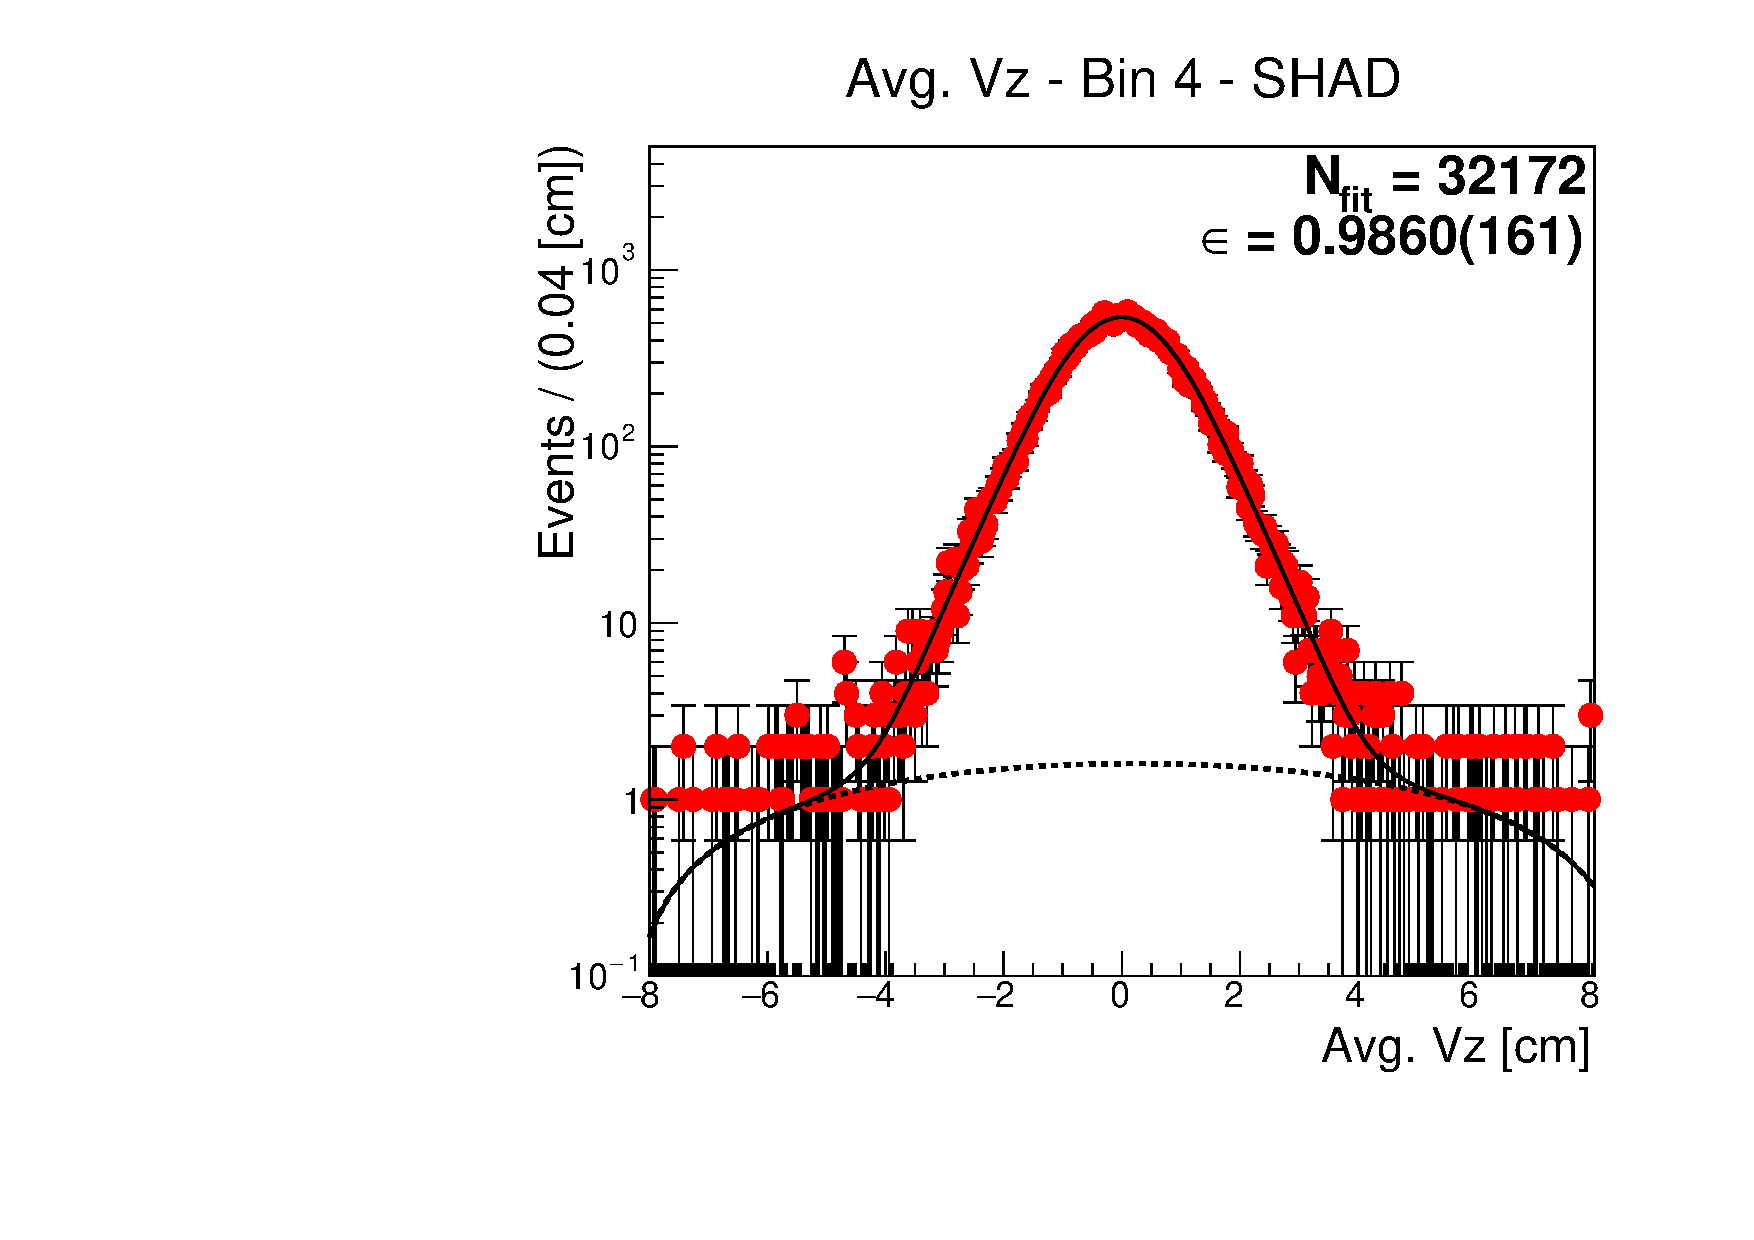
\includegraphics[scale=0.25]{figures/plots/nonDDbar_fit_results/scan/fit_scan_04_data_SHAD.pdf}
\hspace{-0.5cm}
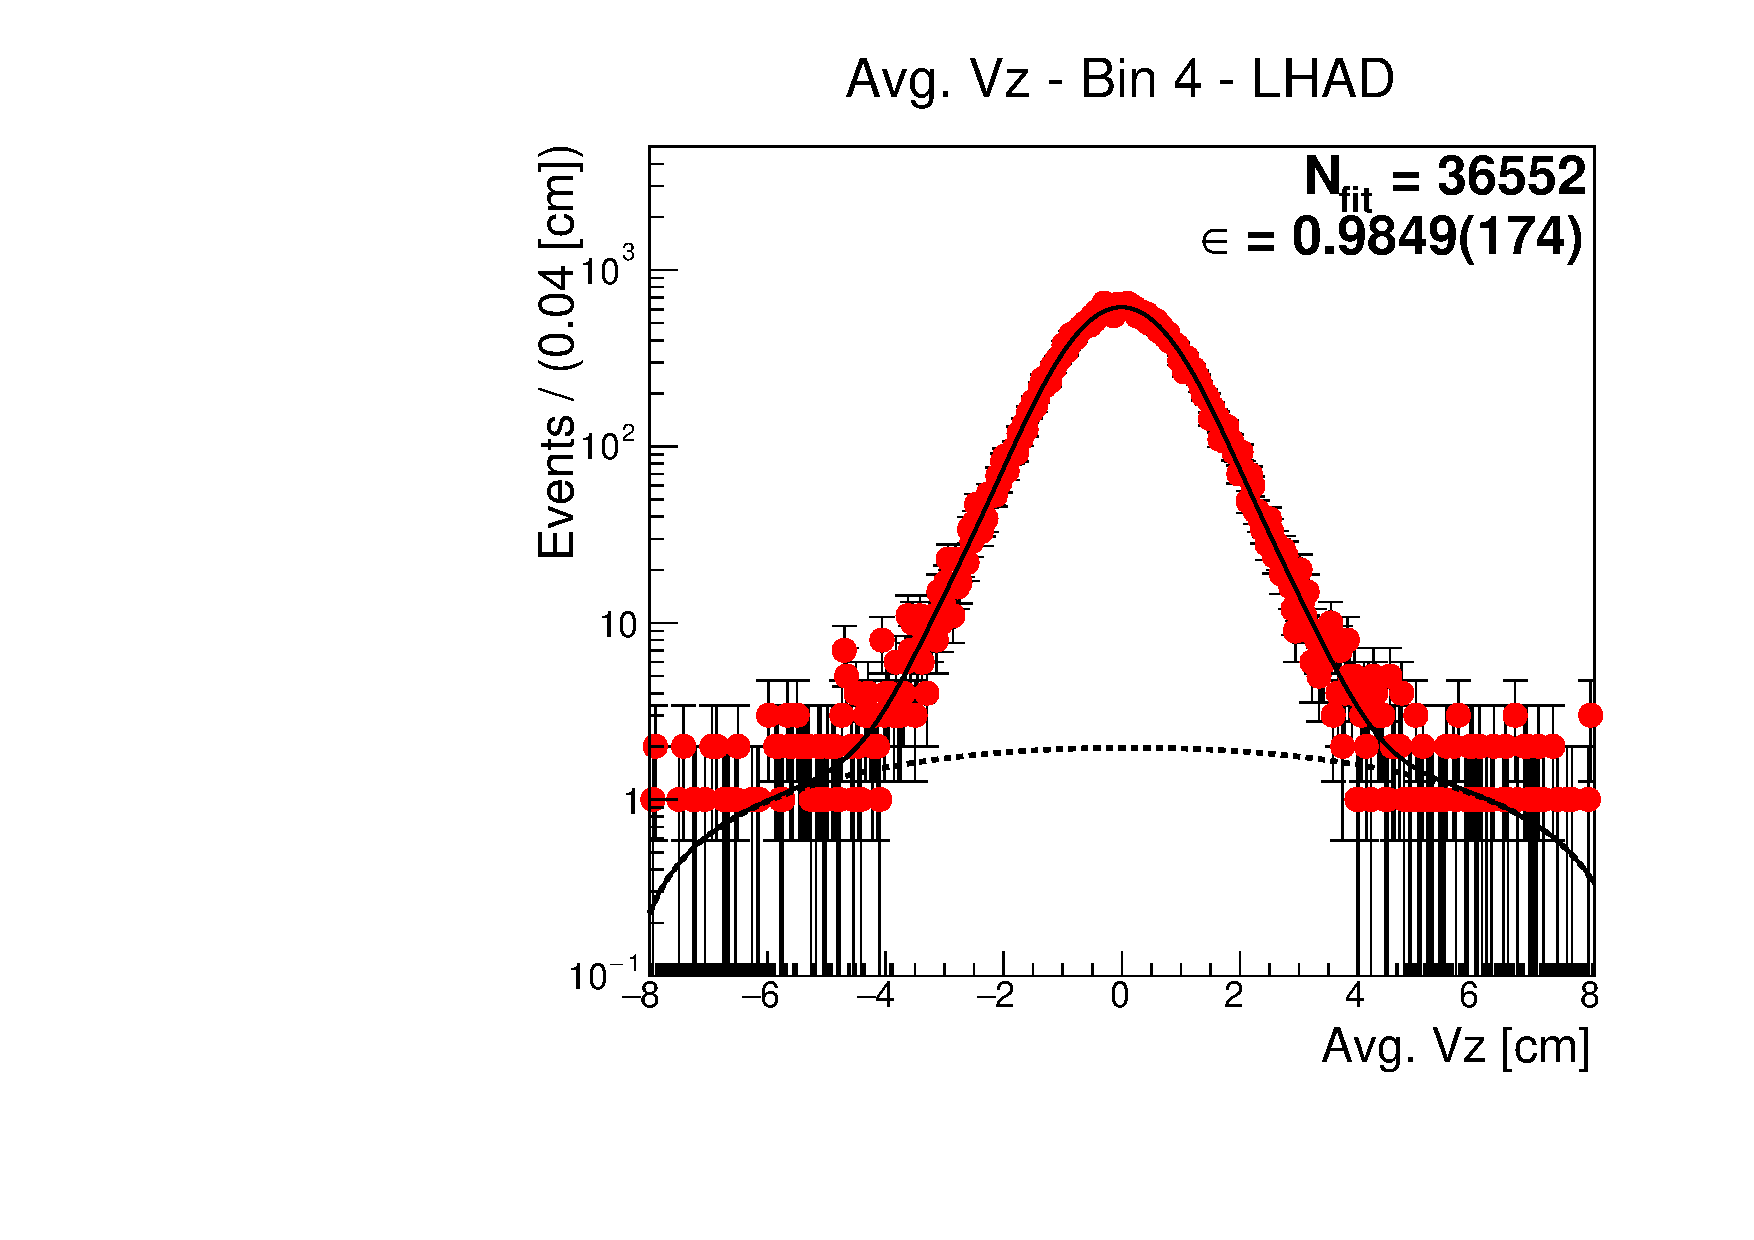
\includegraphics[scale=0.25]{figures/plots/nonDDbar_fit_results/scan/fit_scan_04_data_LHAD.pdf}
\hspace{-0.5cm}
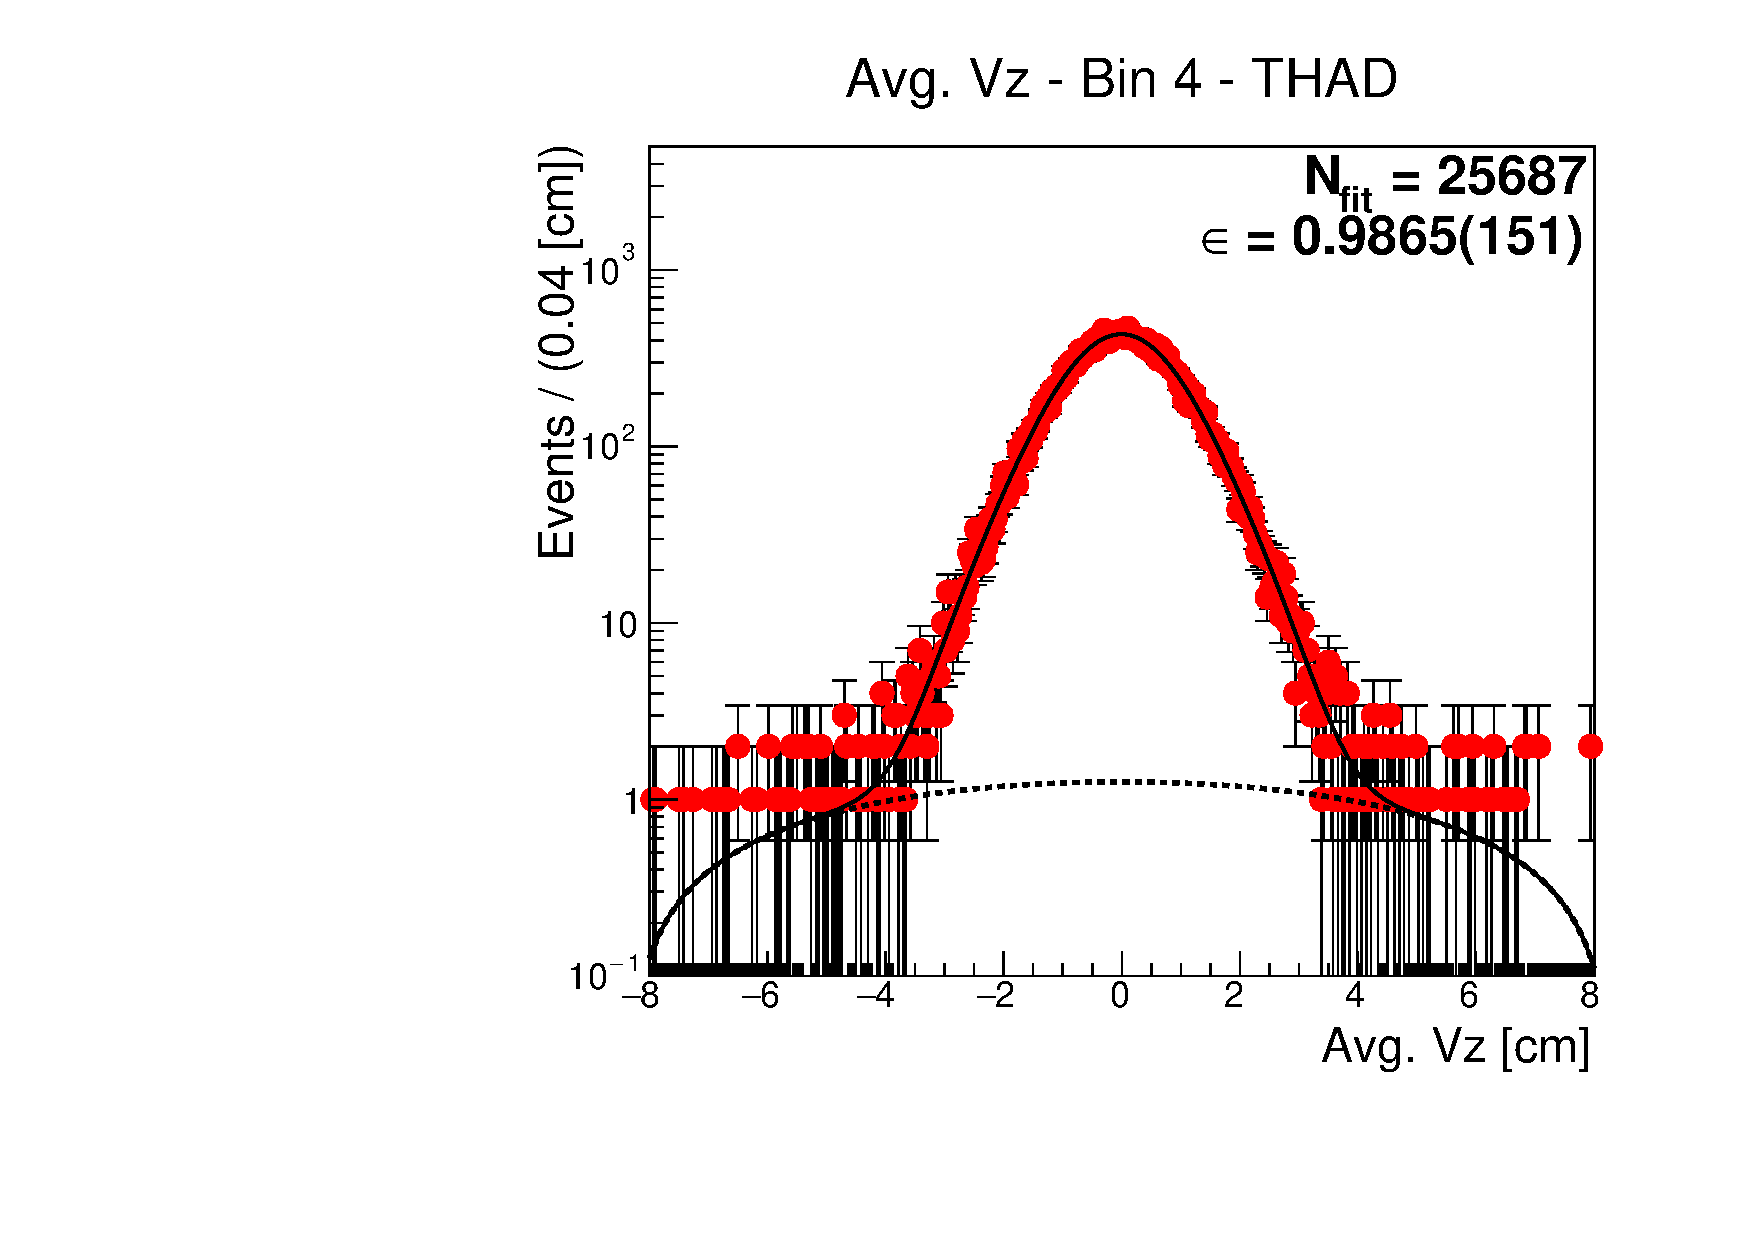
\includegraphics[scale=0.25]{figures/plots/nonDDbar_fit_results/scan/fit_scan_04_data_THAD.pdf}
\caption{Fits to determine the number of hadrons in the 3750 (Scan) data sample.}
{This includes results for SHAD (left), LHAD (middle), and THAD (right).}
\label{fig:hadron_fits_scan_04}
\end{figure}

\begin{figure}[H]
\centering
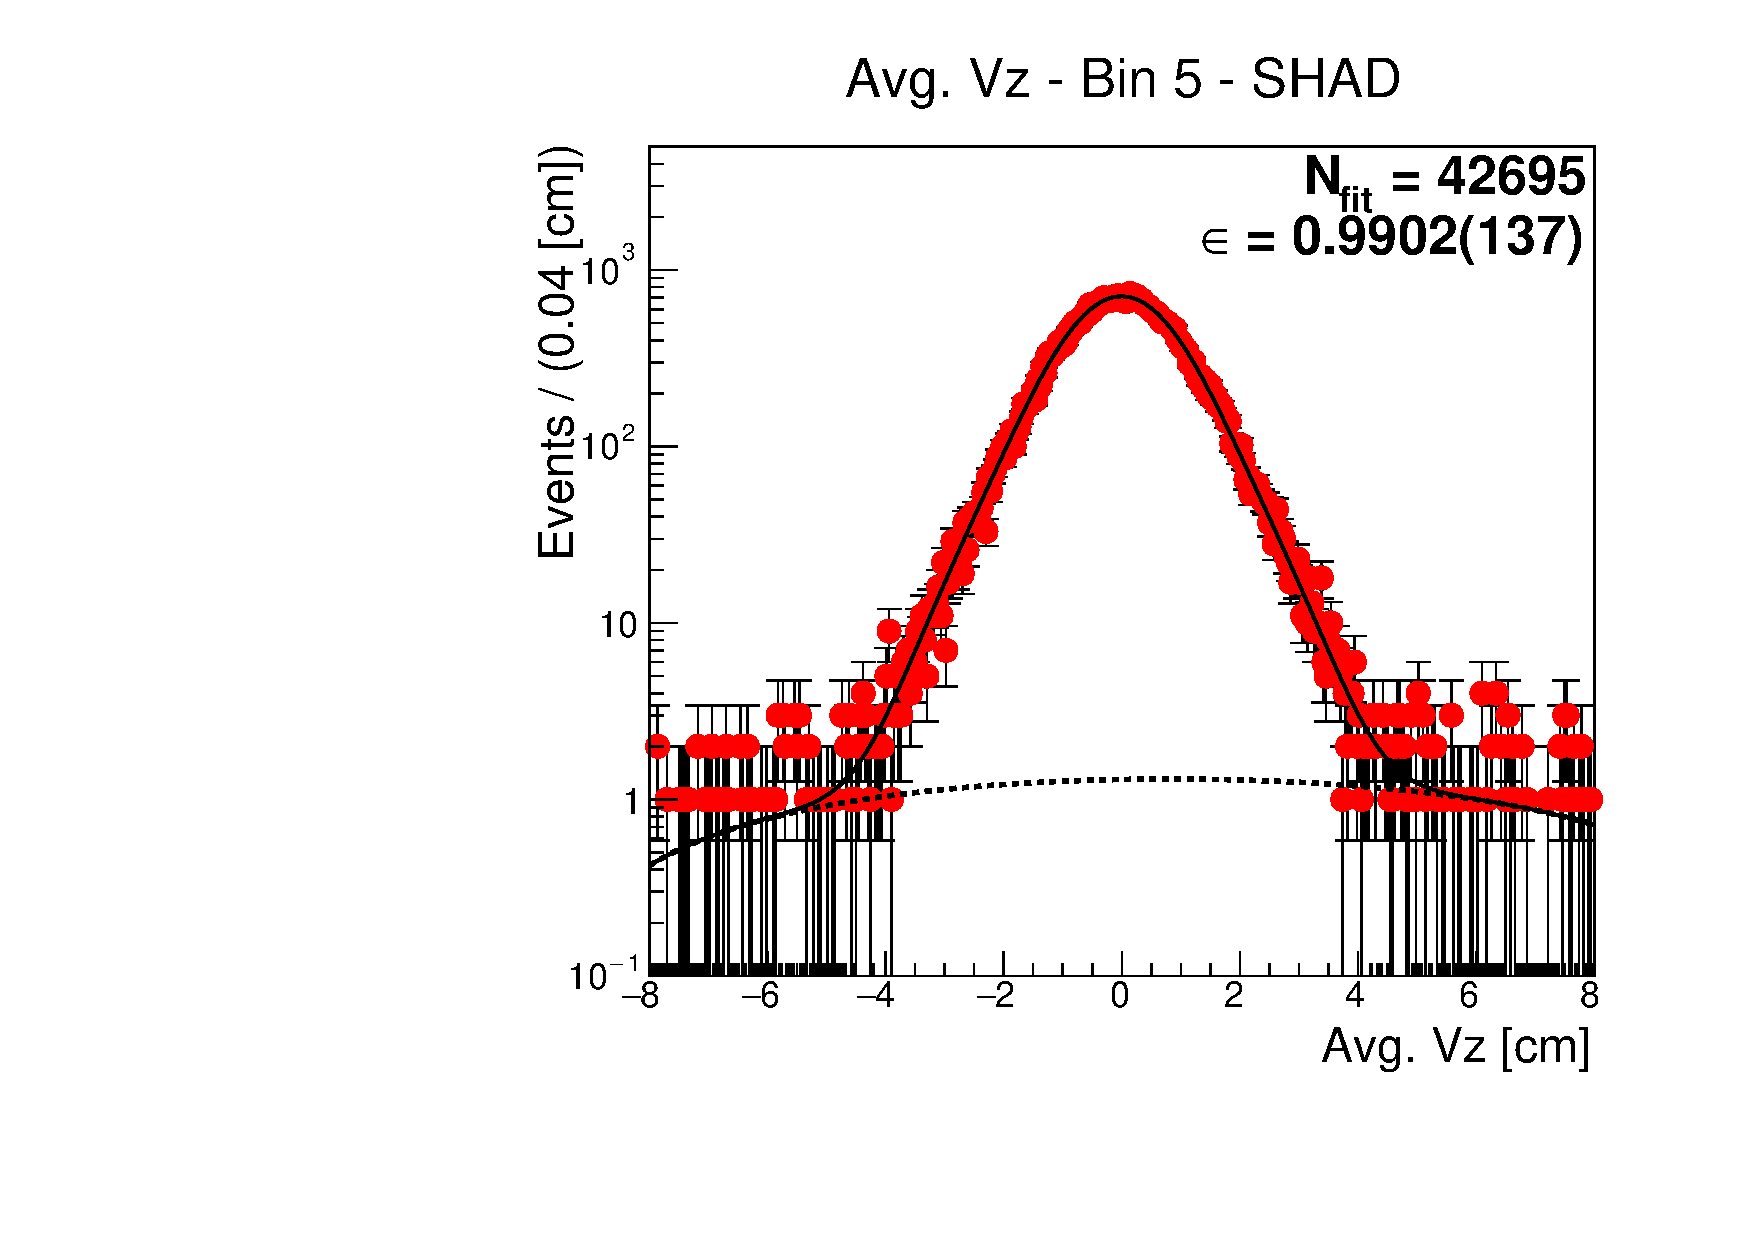
\includegraphics[scale=0.25]{figures/plots/nonDDbar_fit_results/scan/fit_scan_05_data_SHAD.pdf}
\hspace{-0.5cm}
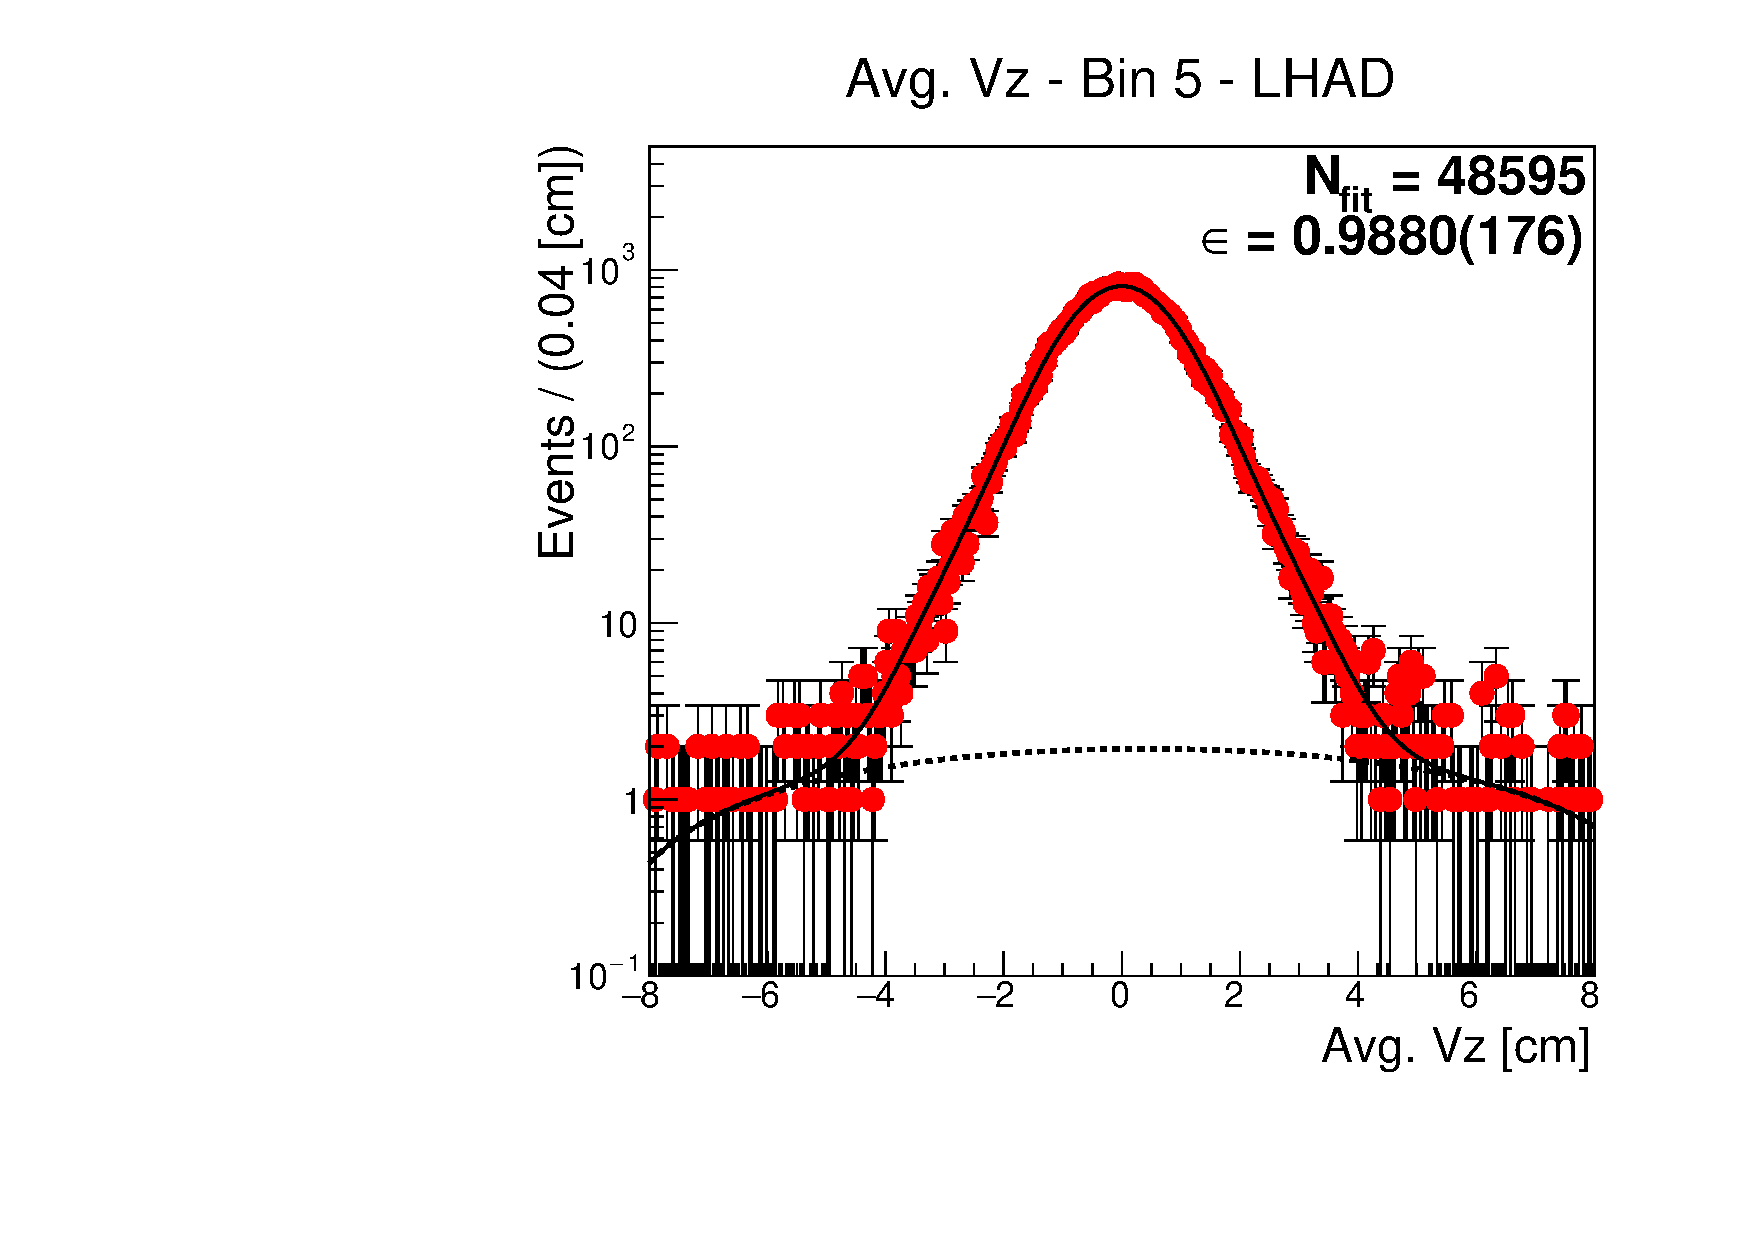
\includegraphics[scale=0.25]{figures/plots/nonDDbar_fit_results/scan/fit_scan_05_data_LHAD.pdf}
\hspace{-0.5cm}
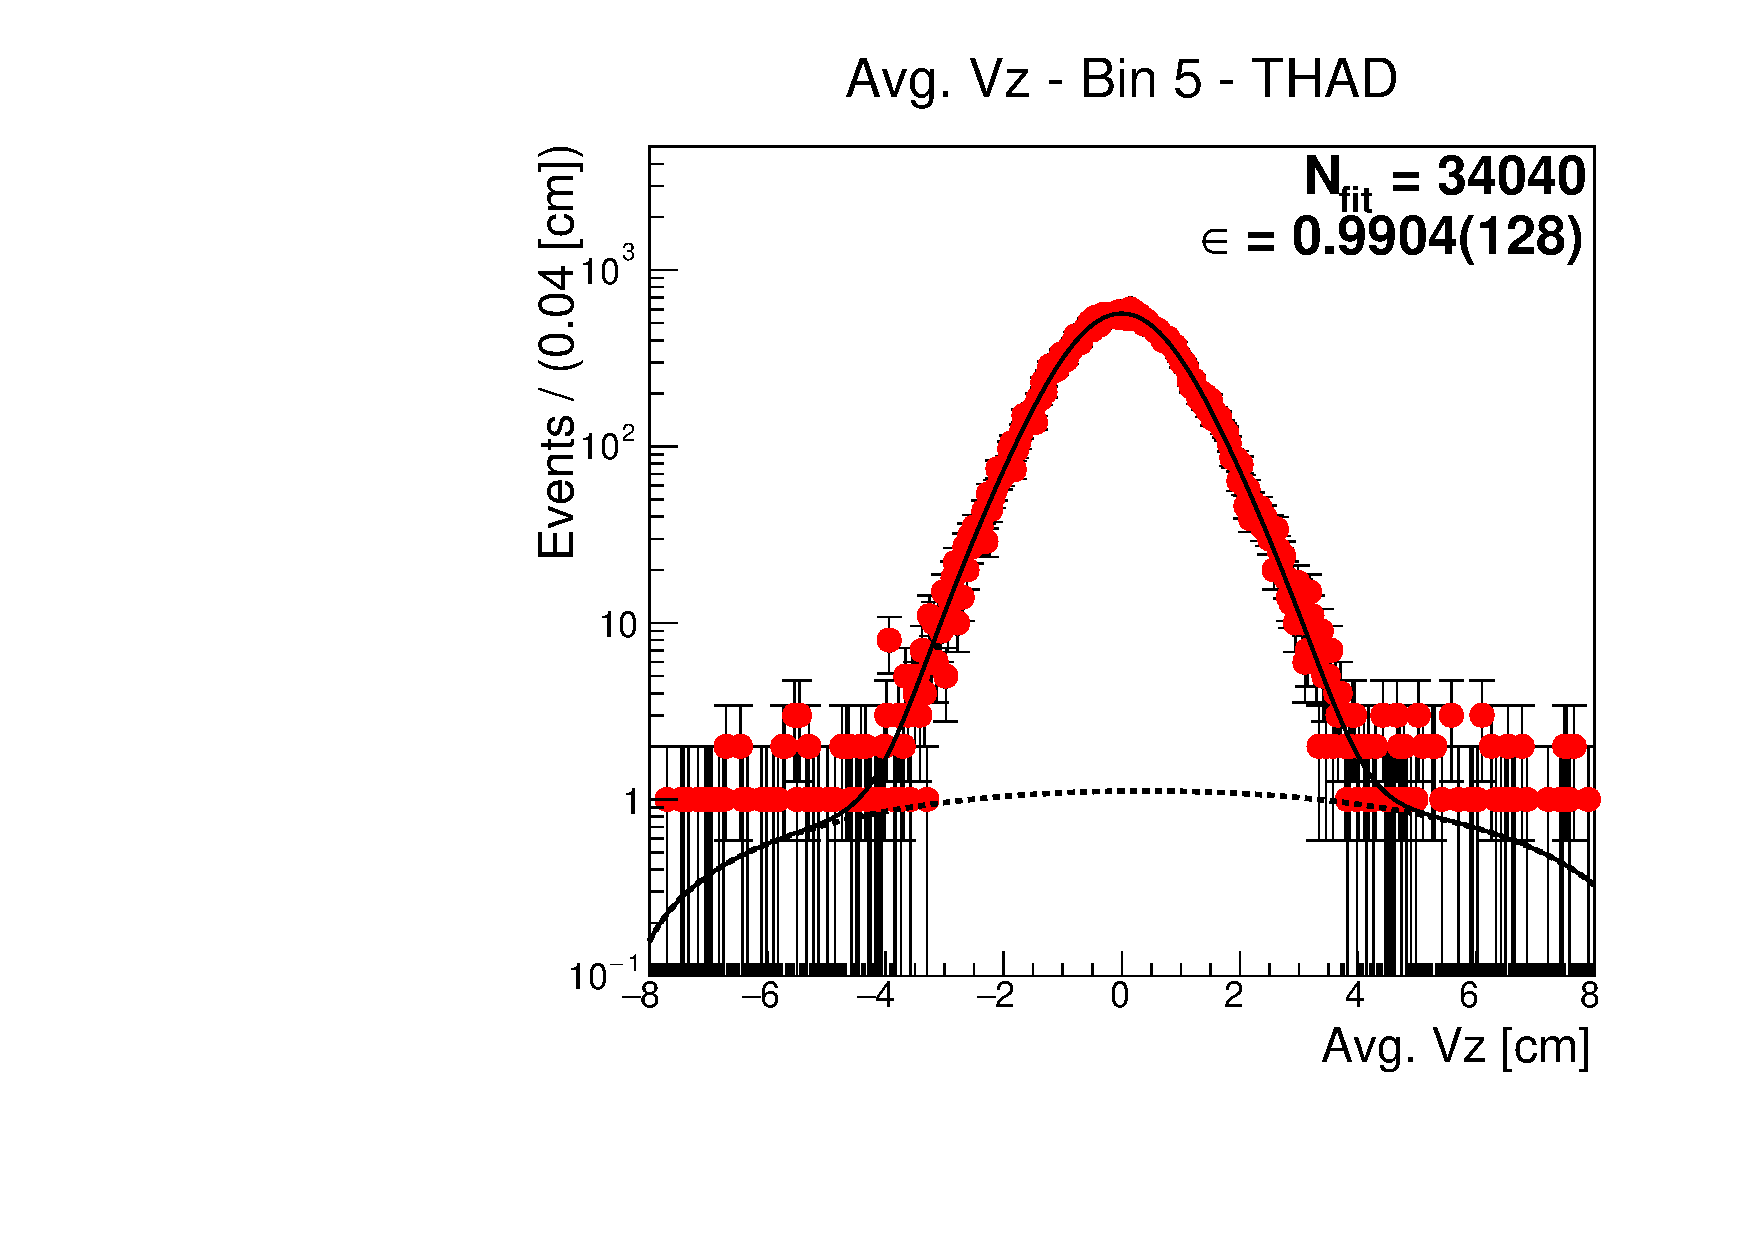
\includegraphics[scale=0.25]{figures/plots/nonDDbar_fit_results/scan/fit_scan_05_data_THAD.pdf}
\caption{Fits to determine the number of hadrons in the 3751 (Scan) data sample.}
{This includes results for SHAD (left), LHAD (middle), and THAD (right).}
\label{fig:hadron_fits_scan_05}
\end{figure}

\begin{figure}[H]
\centering
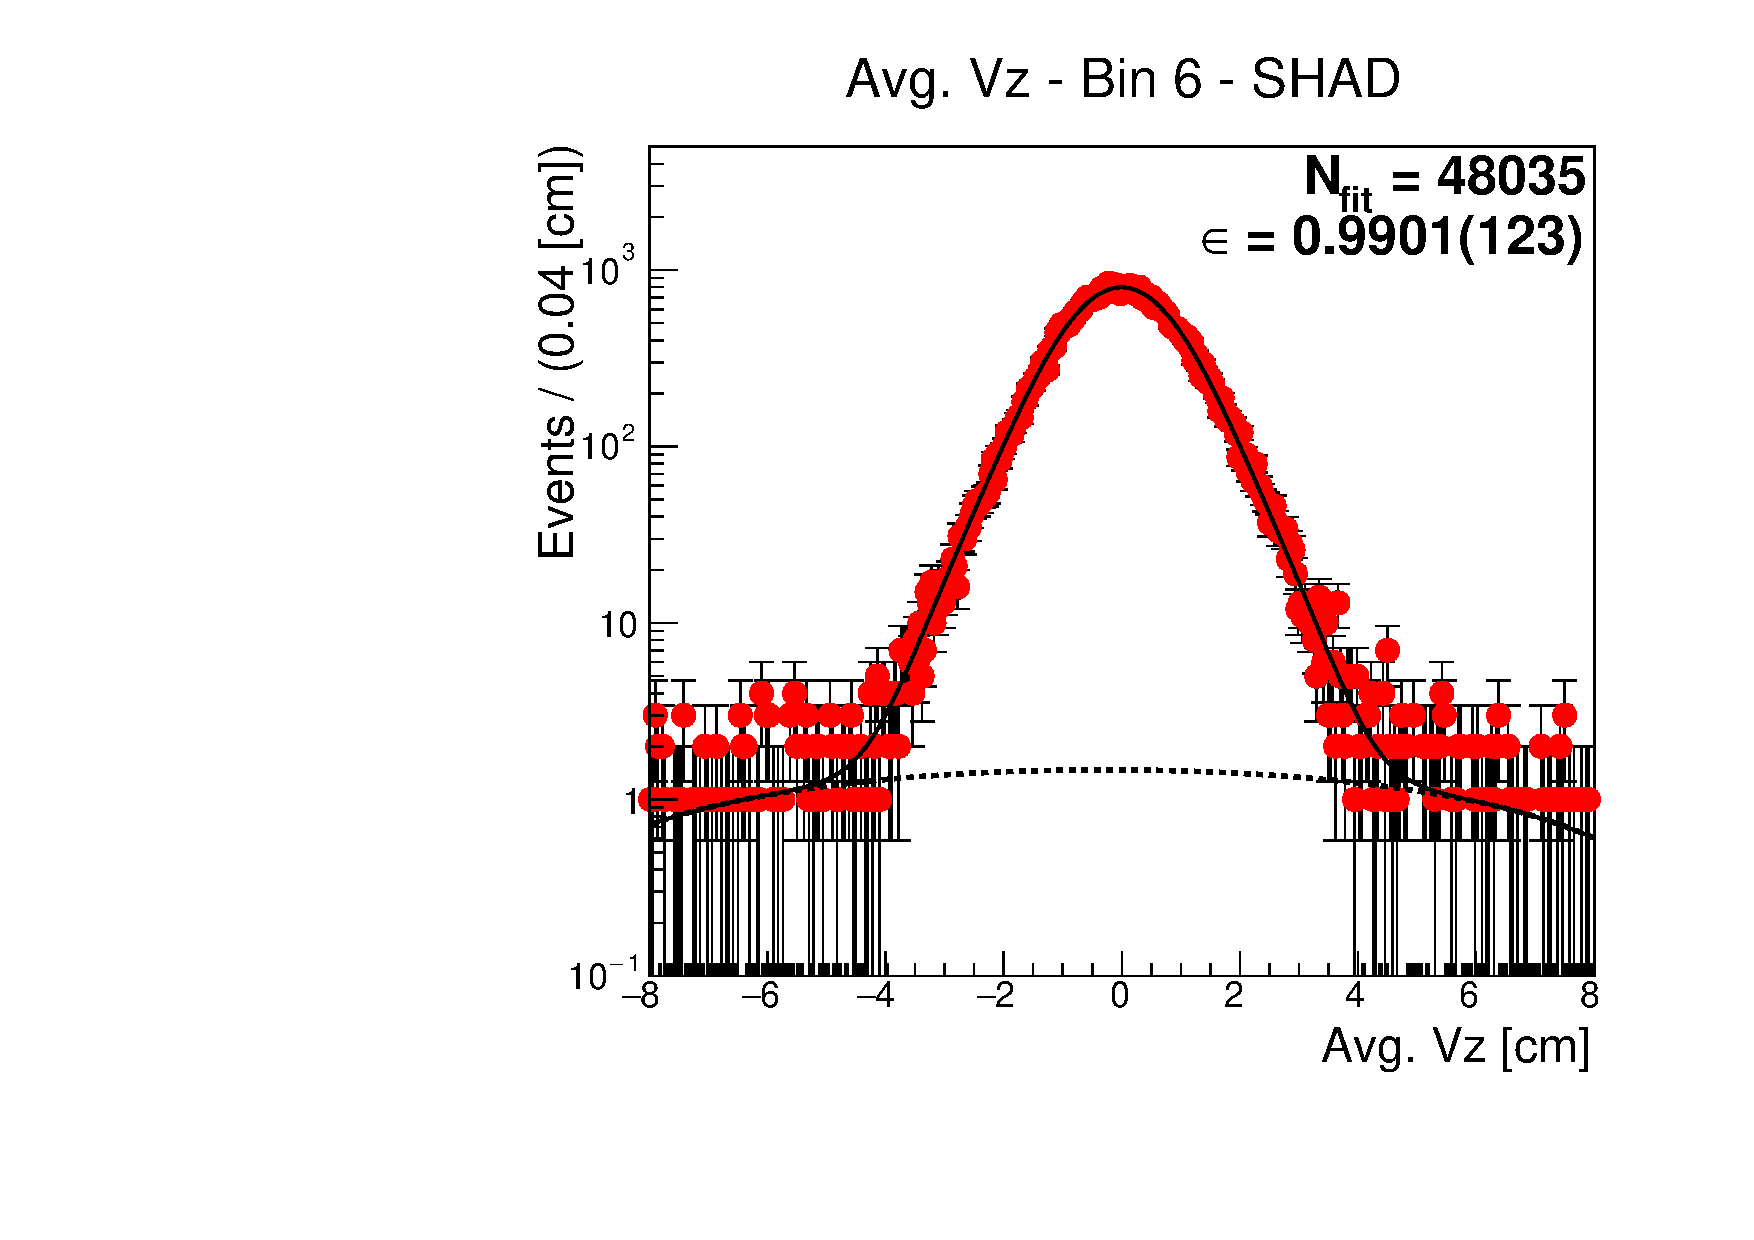
\includegraphics[scale=0.25]{figures/plots/nonDDbar_fit_results/scan/fit_scan_06_data_SHAD.pdf}
\hspace{-0.5cm}
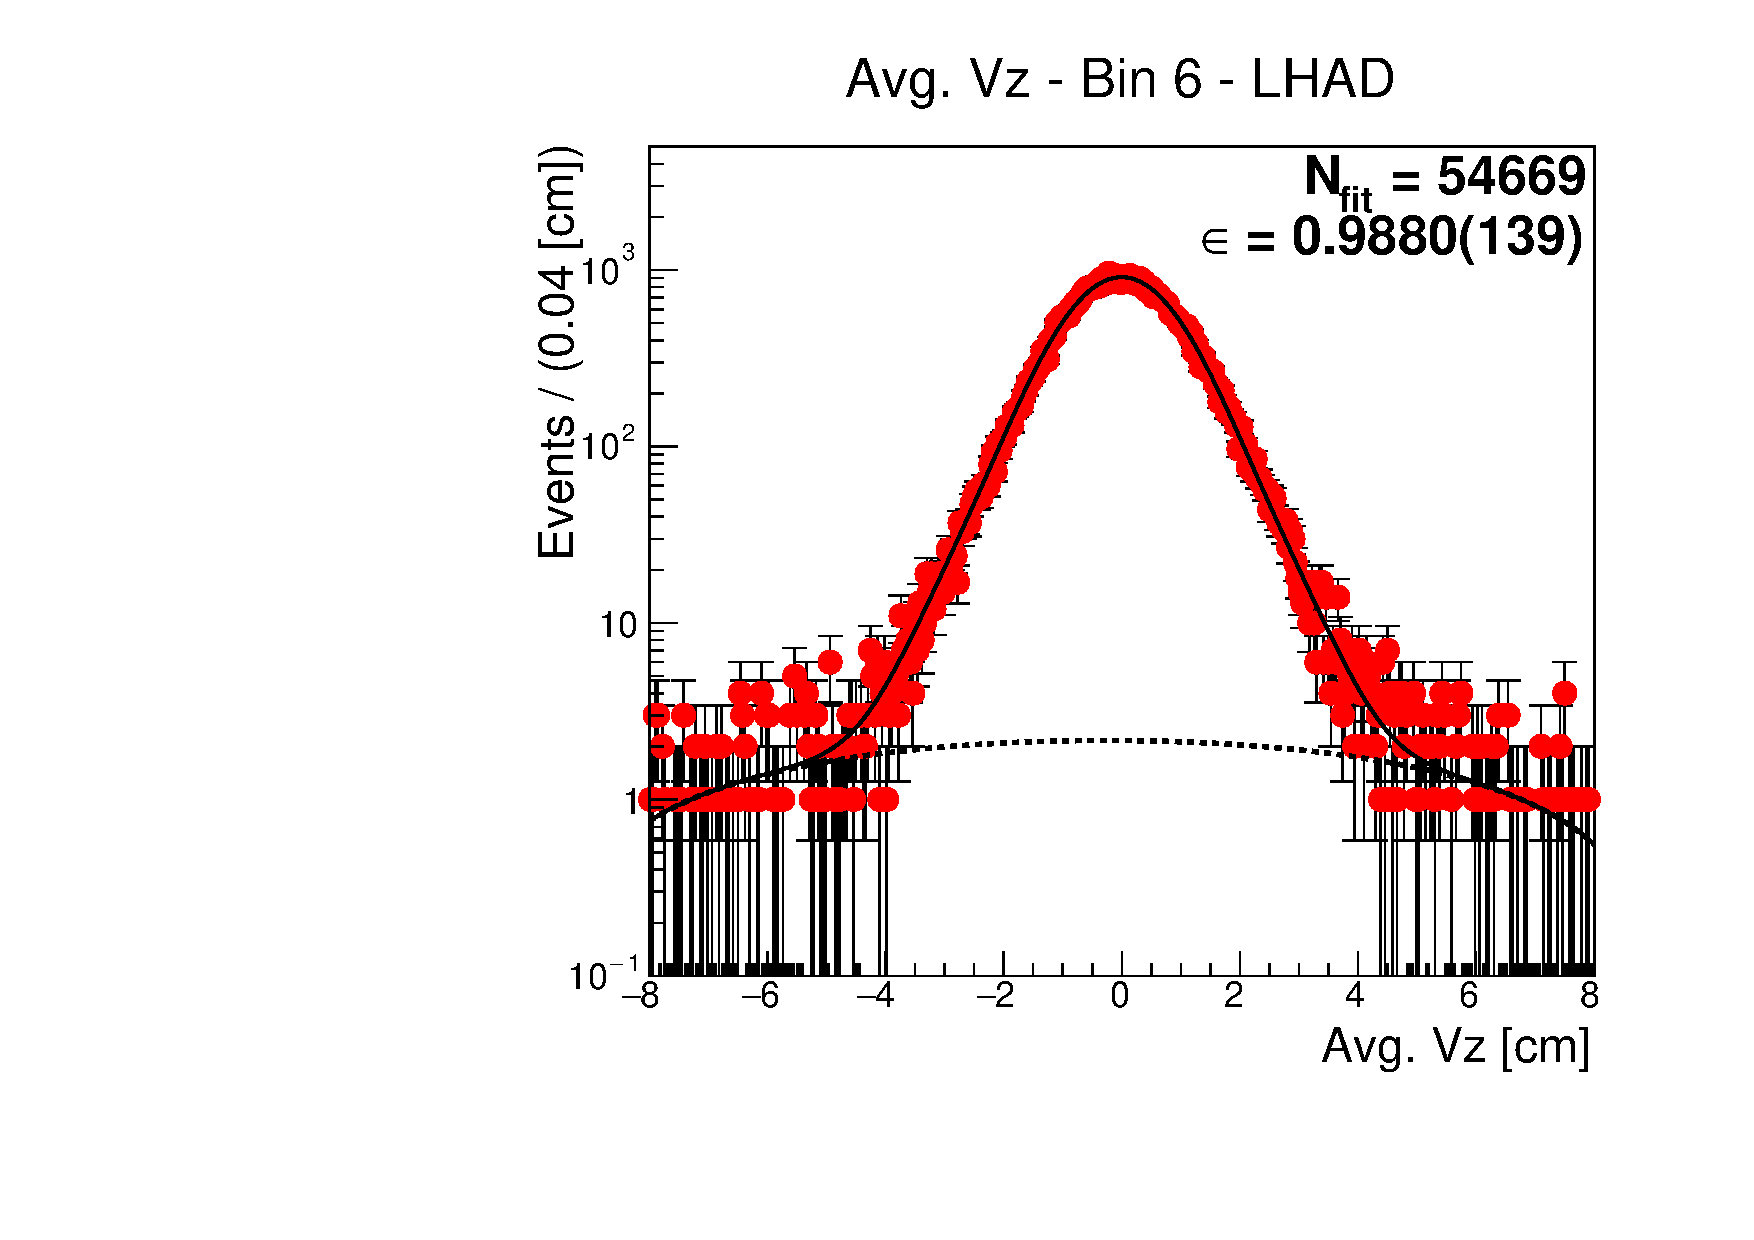
\includegraphics[scale=0.25]{figures/plots/nonDDbar_fit_results/scan/fit_scan_06_data_LHAD.pdf}
\hspace{-0.5cm}
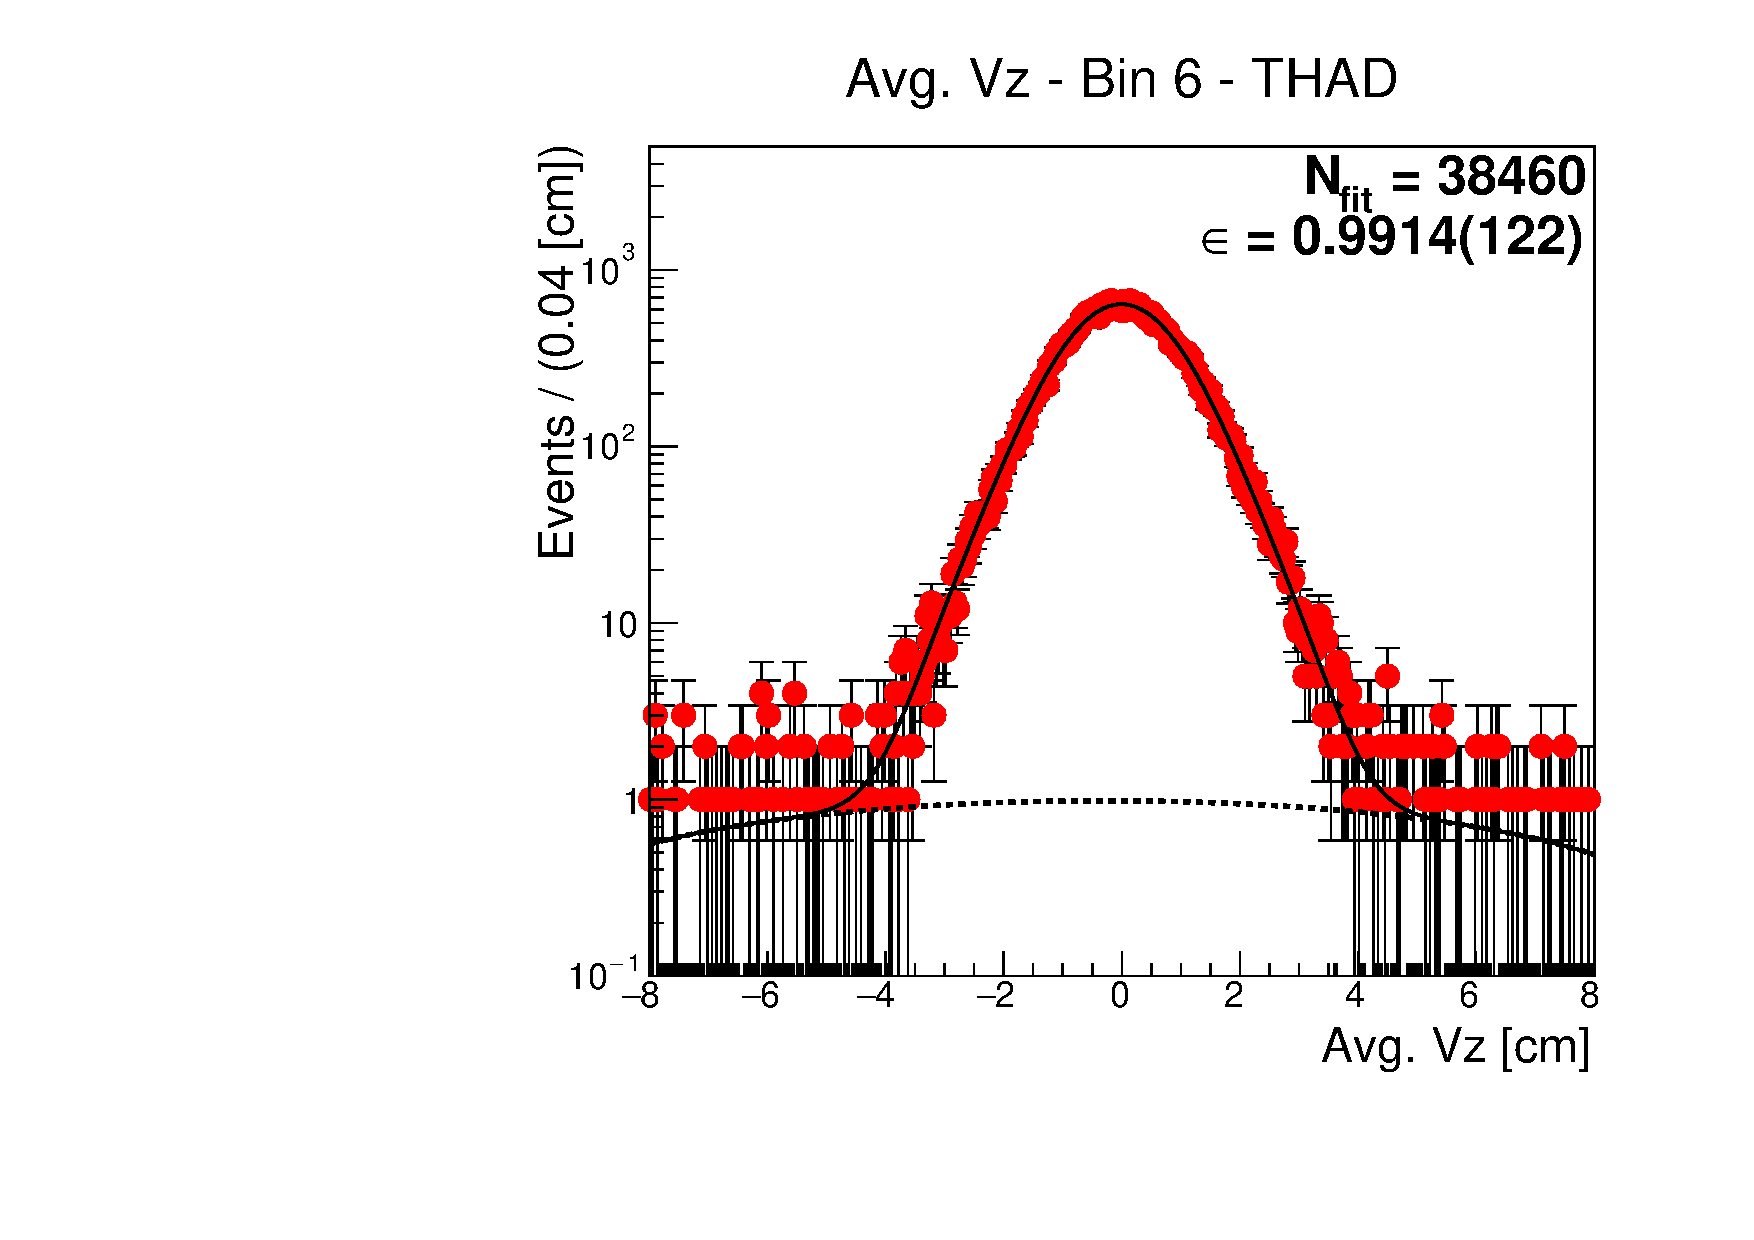
\includegraphics[scale=0.25]{figures/plots/nonDDbar_fit_results/scan/fit_scan_06_data_THAD.pdf}
\caption{Fits to determine the number of hadrons in the 3753 (Scan) data sample.}
{This includes results for SHAD (left), LHAD (middle), and THAD (right).}
\label{fig:hadron_fits_scan_06}
\end{figure}

\begin{figure}[H]
\centering
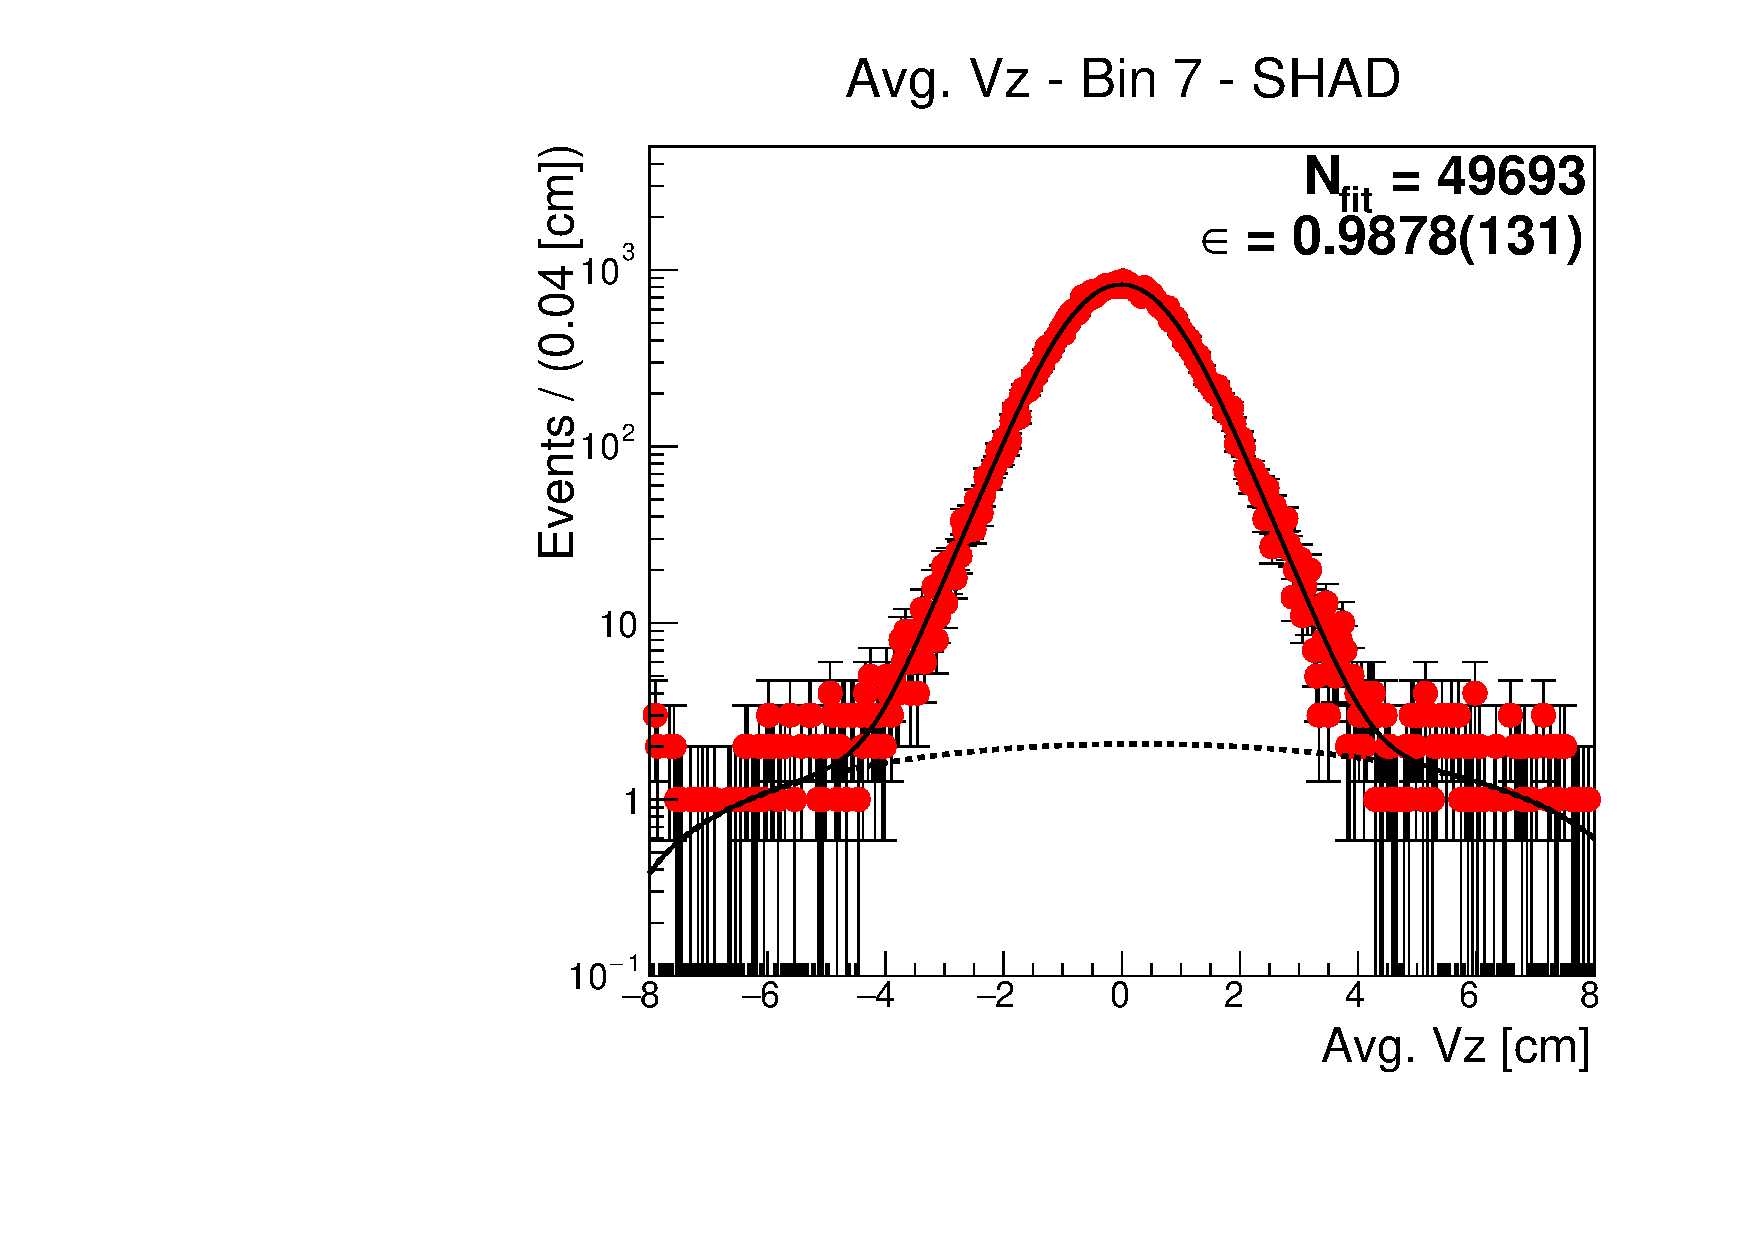
\includegraphics[scale=0.25]{figures/plots/nonDDbar_fit_results/scan/fit_scan_07_data_SHAD.pdf}
\hspace{-0.5cm}
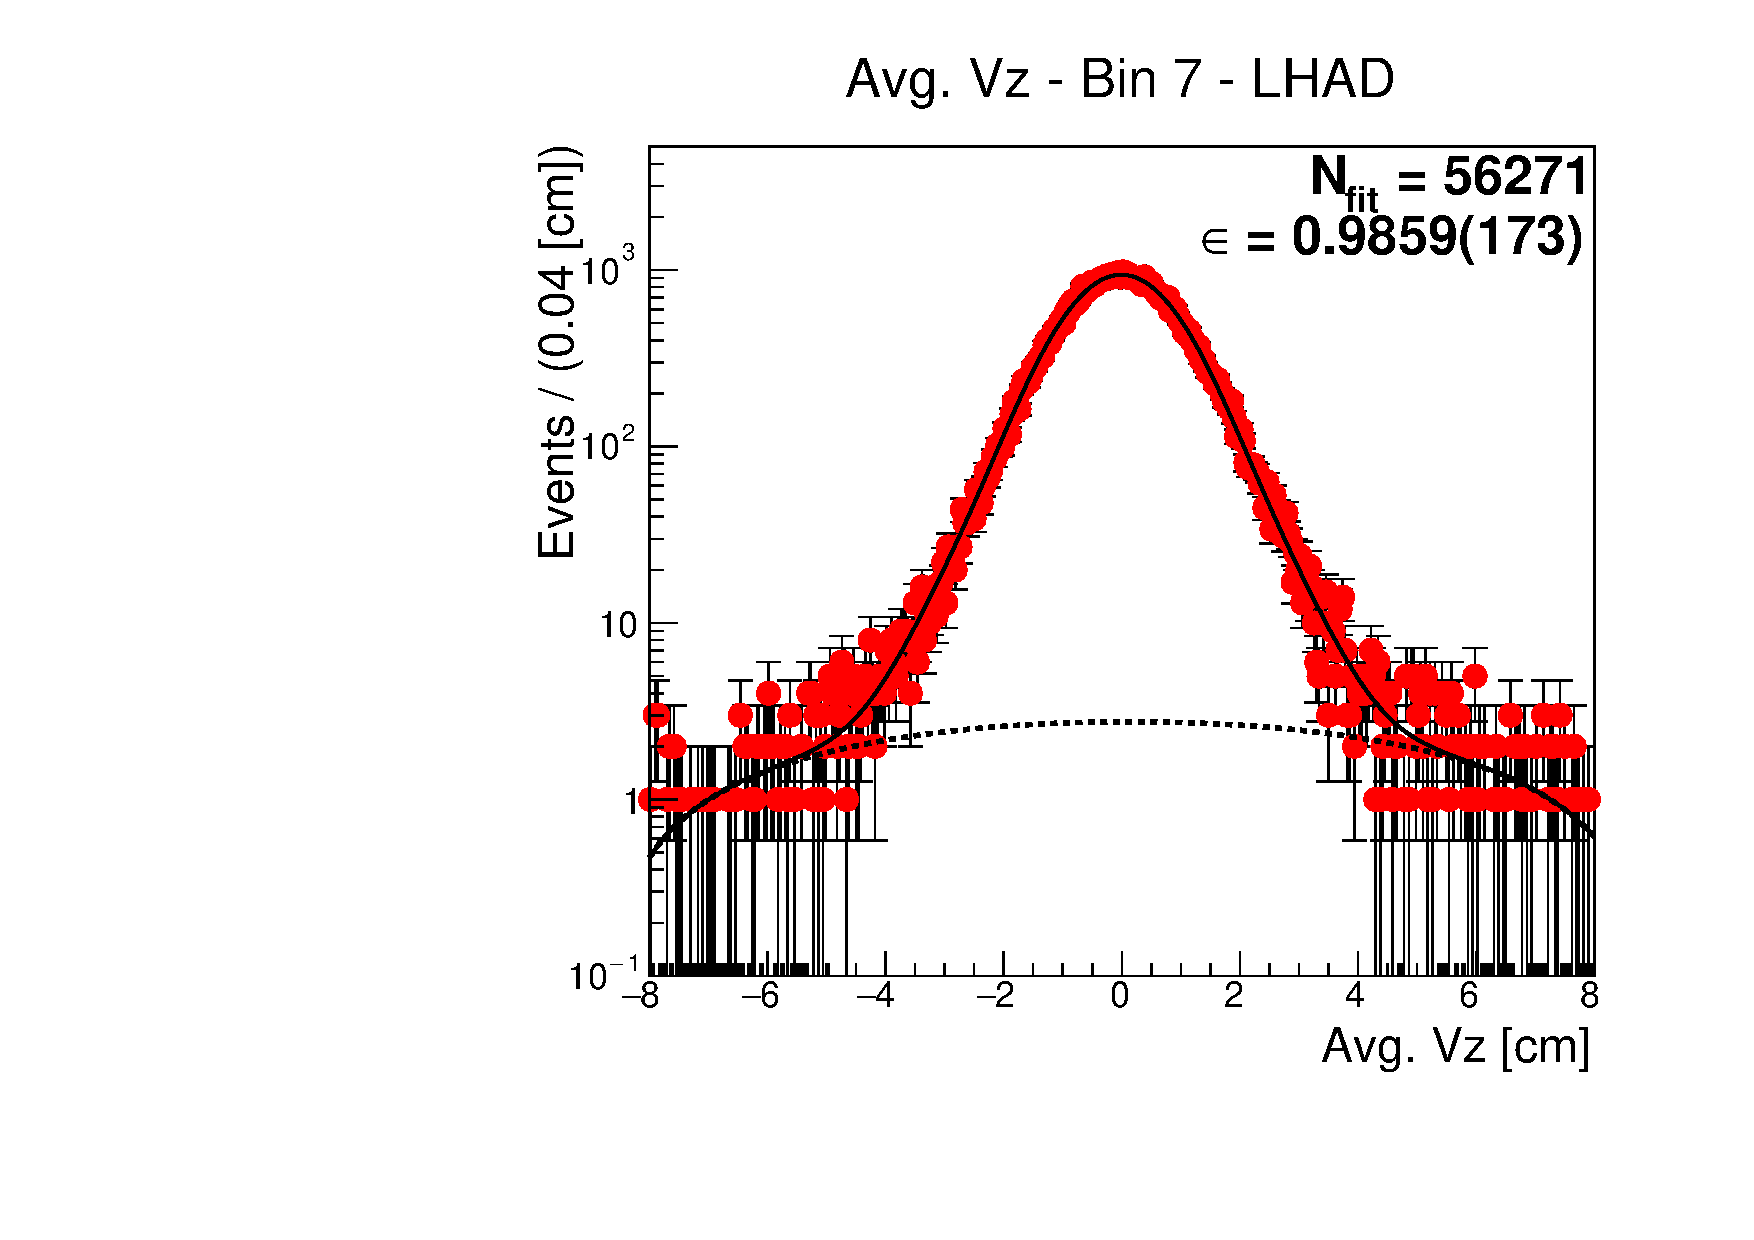
\includegraphics[scale=0.25]{figures/plots/nonDDbar_fit_results/scan/fit_scan_07_data_LHAD.pdf}
\hspace{-0.5cm}
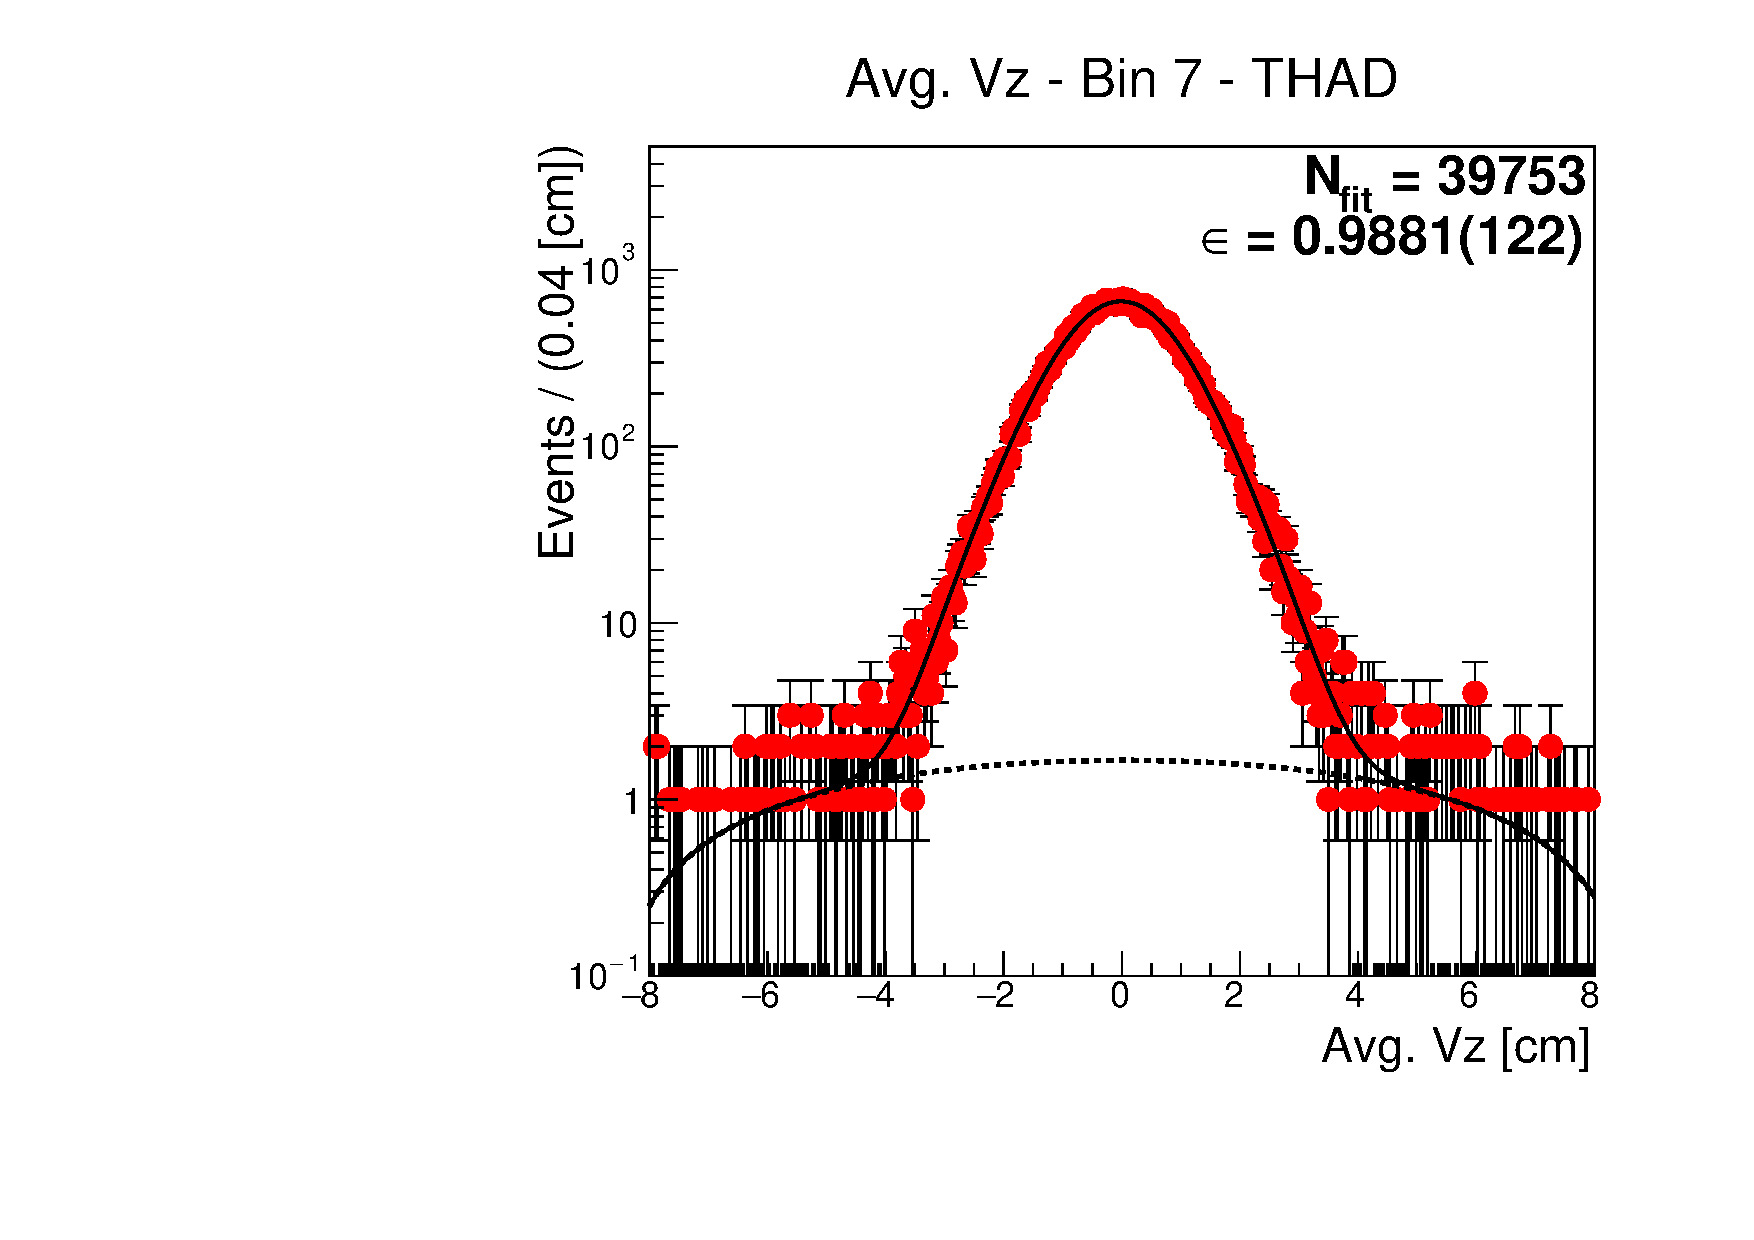
\includegraphics[scale=0.25]{figures/plots/nonDDbar_fit_results/scan/fit_scan_07_data_THAD.pdf}
\caption{Fits to determine the number of hadrons in the 3755 (Scan) data sample.}
{This includes results for SHAD (left), LHAD (middle), and THAD (right).}
\label{fig:hadron_fits_scan_07}
\end{figure}

\begin{figure}[H]
\centering
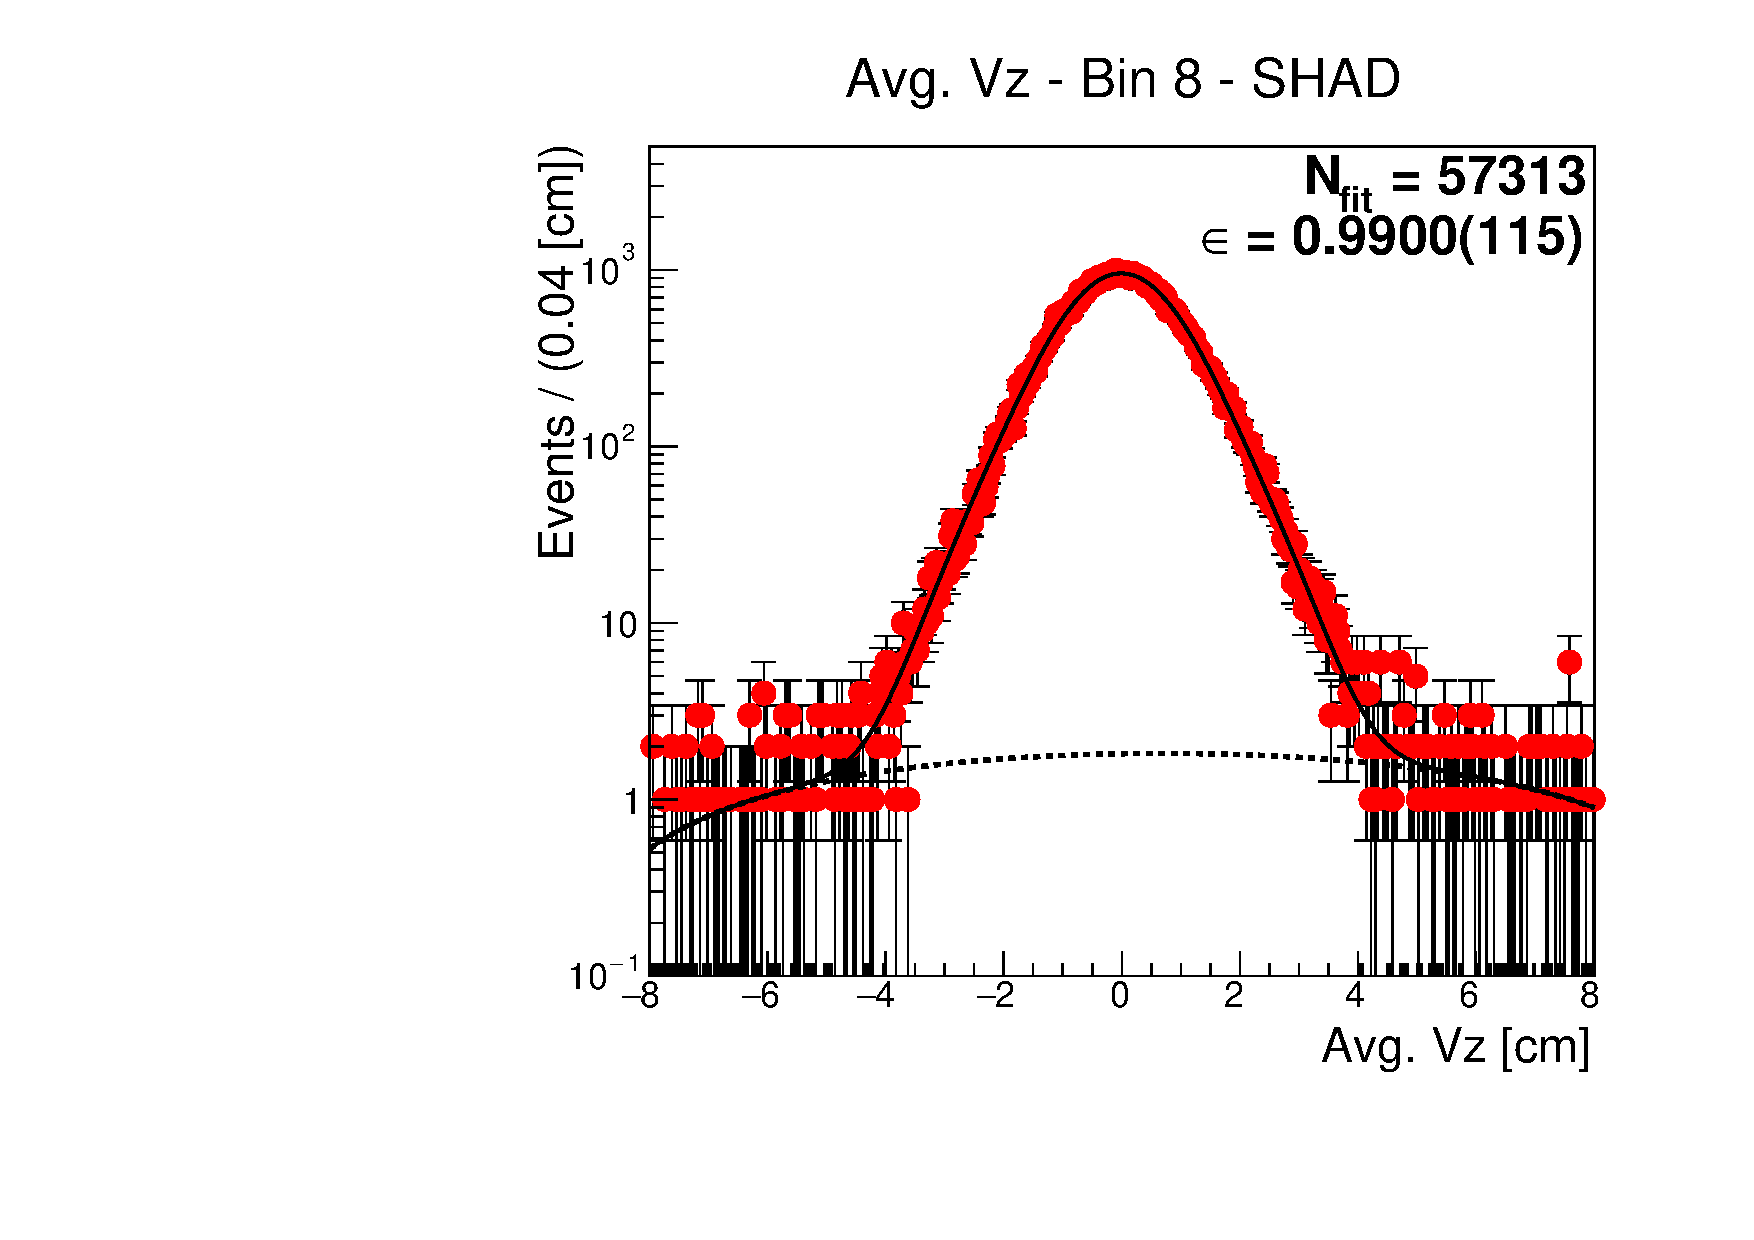
\includegraphics[scale=0.25]{figures/plots/nonDDbar_fit_results/scan/fit_scan_08_data_SHAD.pdf}
\hspace{-0.5cm}
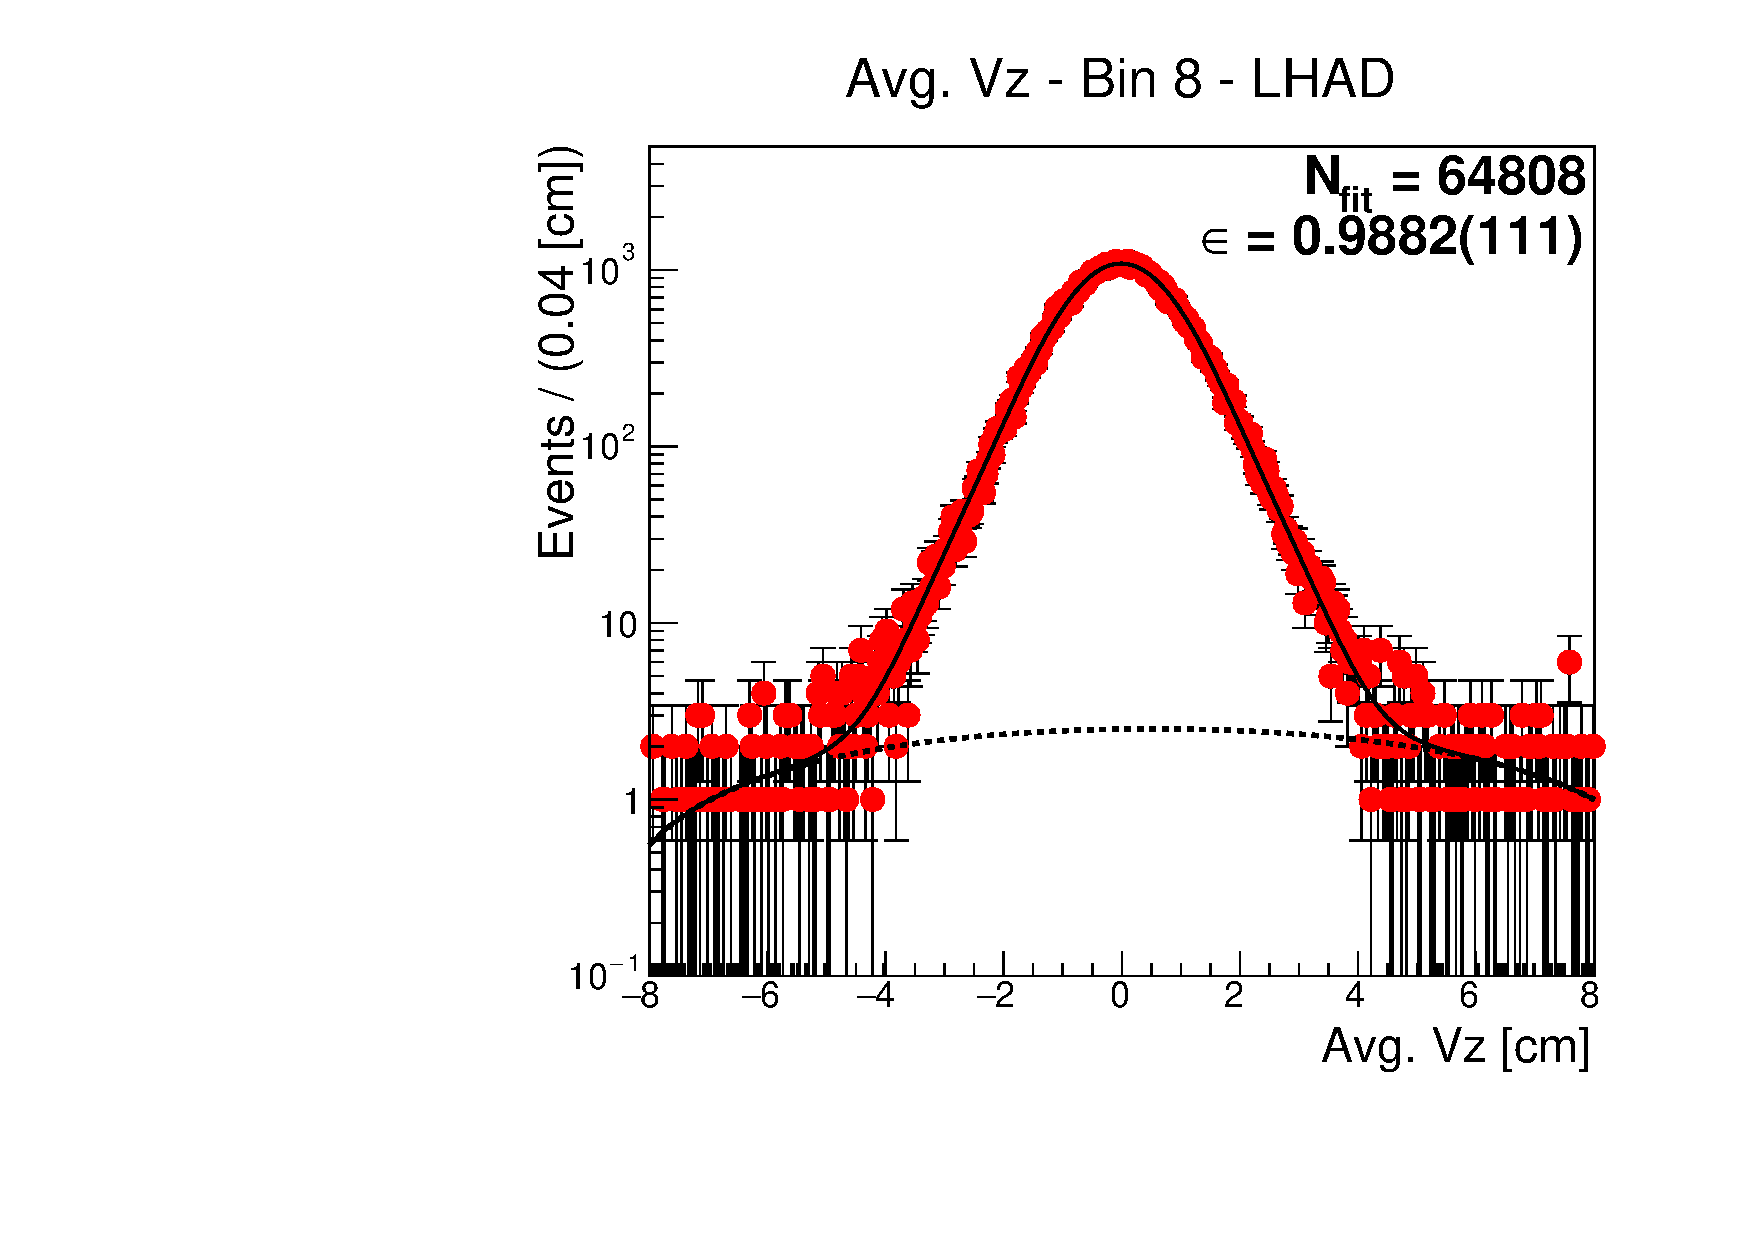
\includegraphics[scale=0.25]{figures/plots/nonDDbar_fit_results/scan/fit_scan_08_data_LHAD.pdf}
\hspace{-0.5cm}
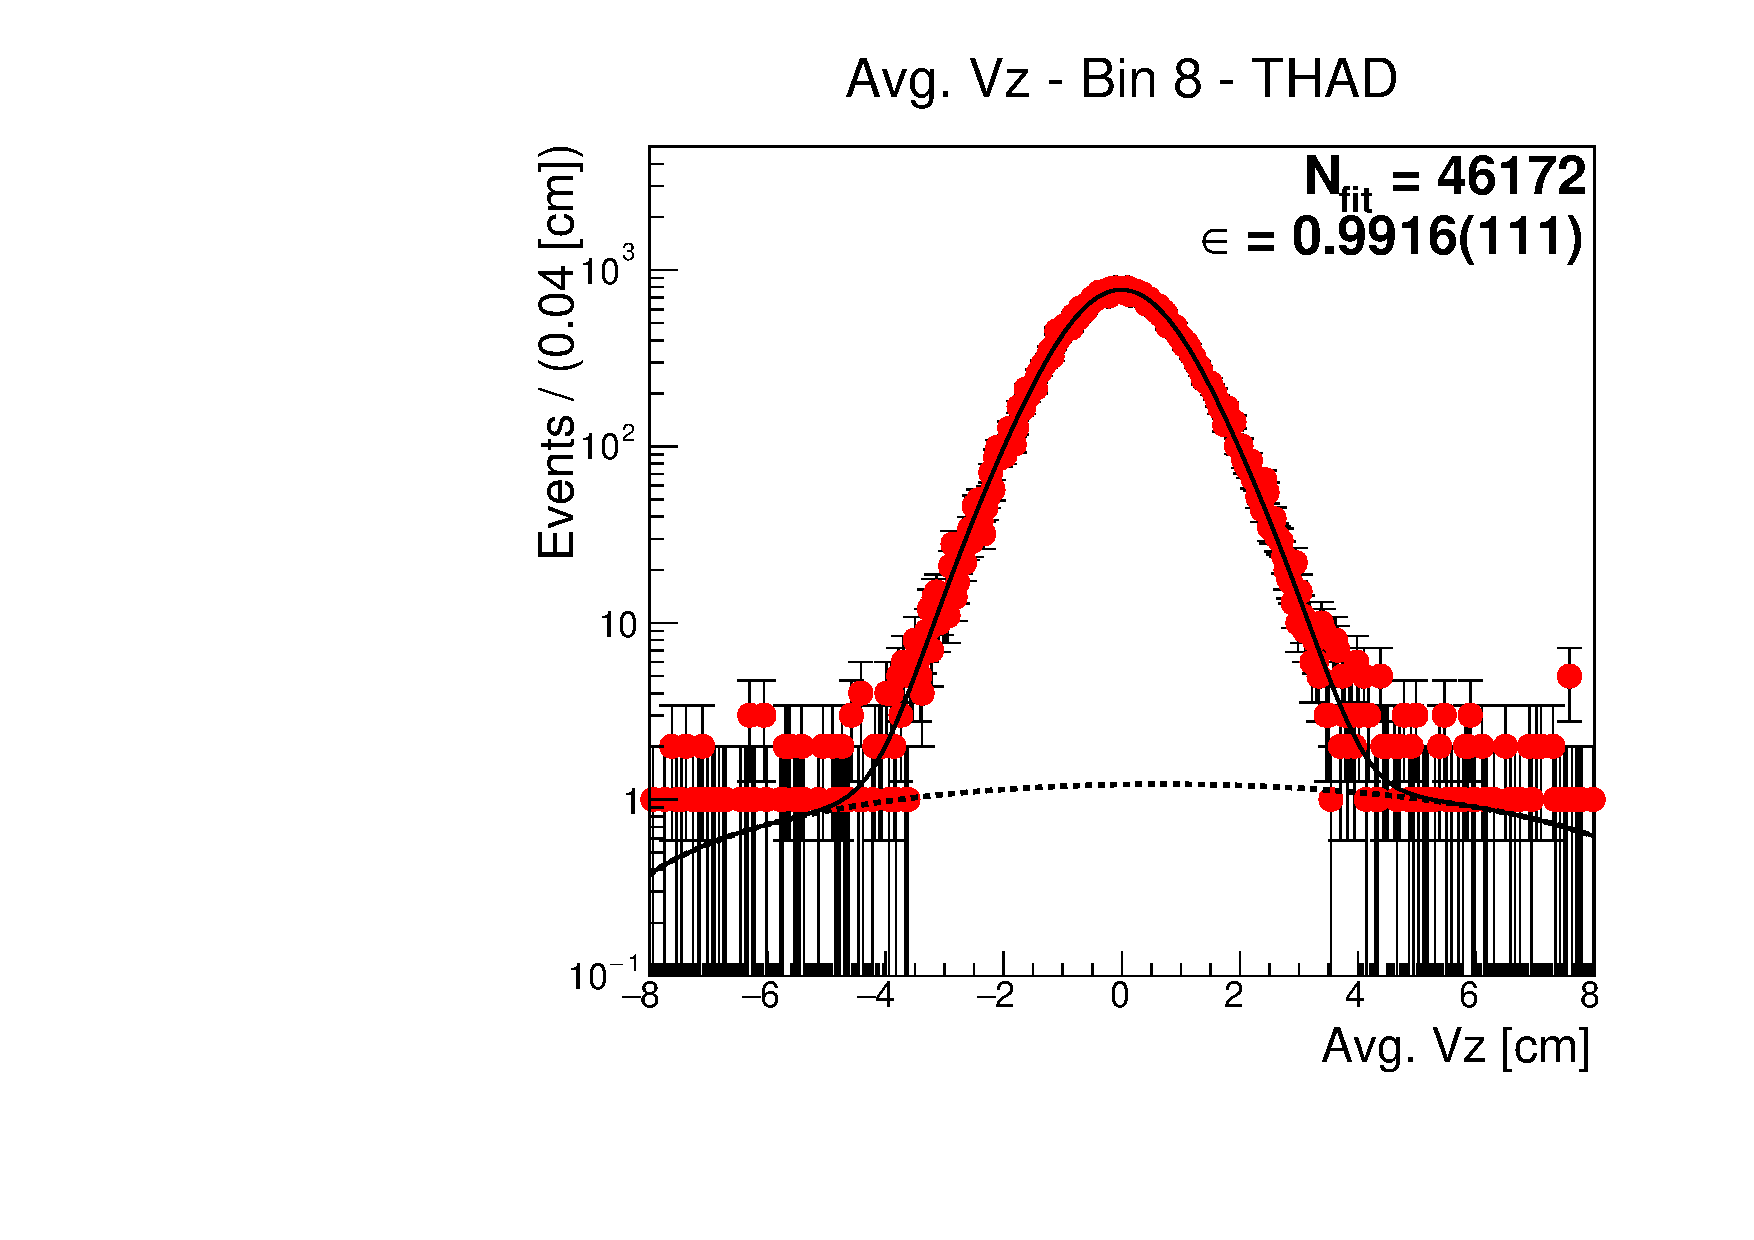
\includegraphics[scale=0.25]{figures/plots/nonDDbar_fit_results/scan/fit_scan_08_data_THAD.pdf}
\caption{Fits to determine the number of hadrons in the 3756 (Scan) data sample.}
{This includes results for SHAD (left), LHAD (middle), and THAD (right).}
\label{fig:hadron_fits_scan_08}
\end{figure}

\begin{figure}[H]
\centering
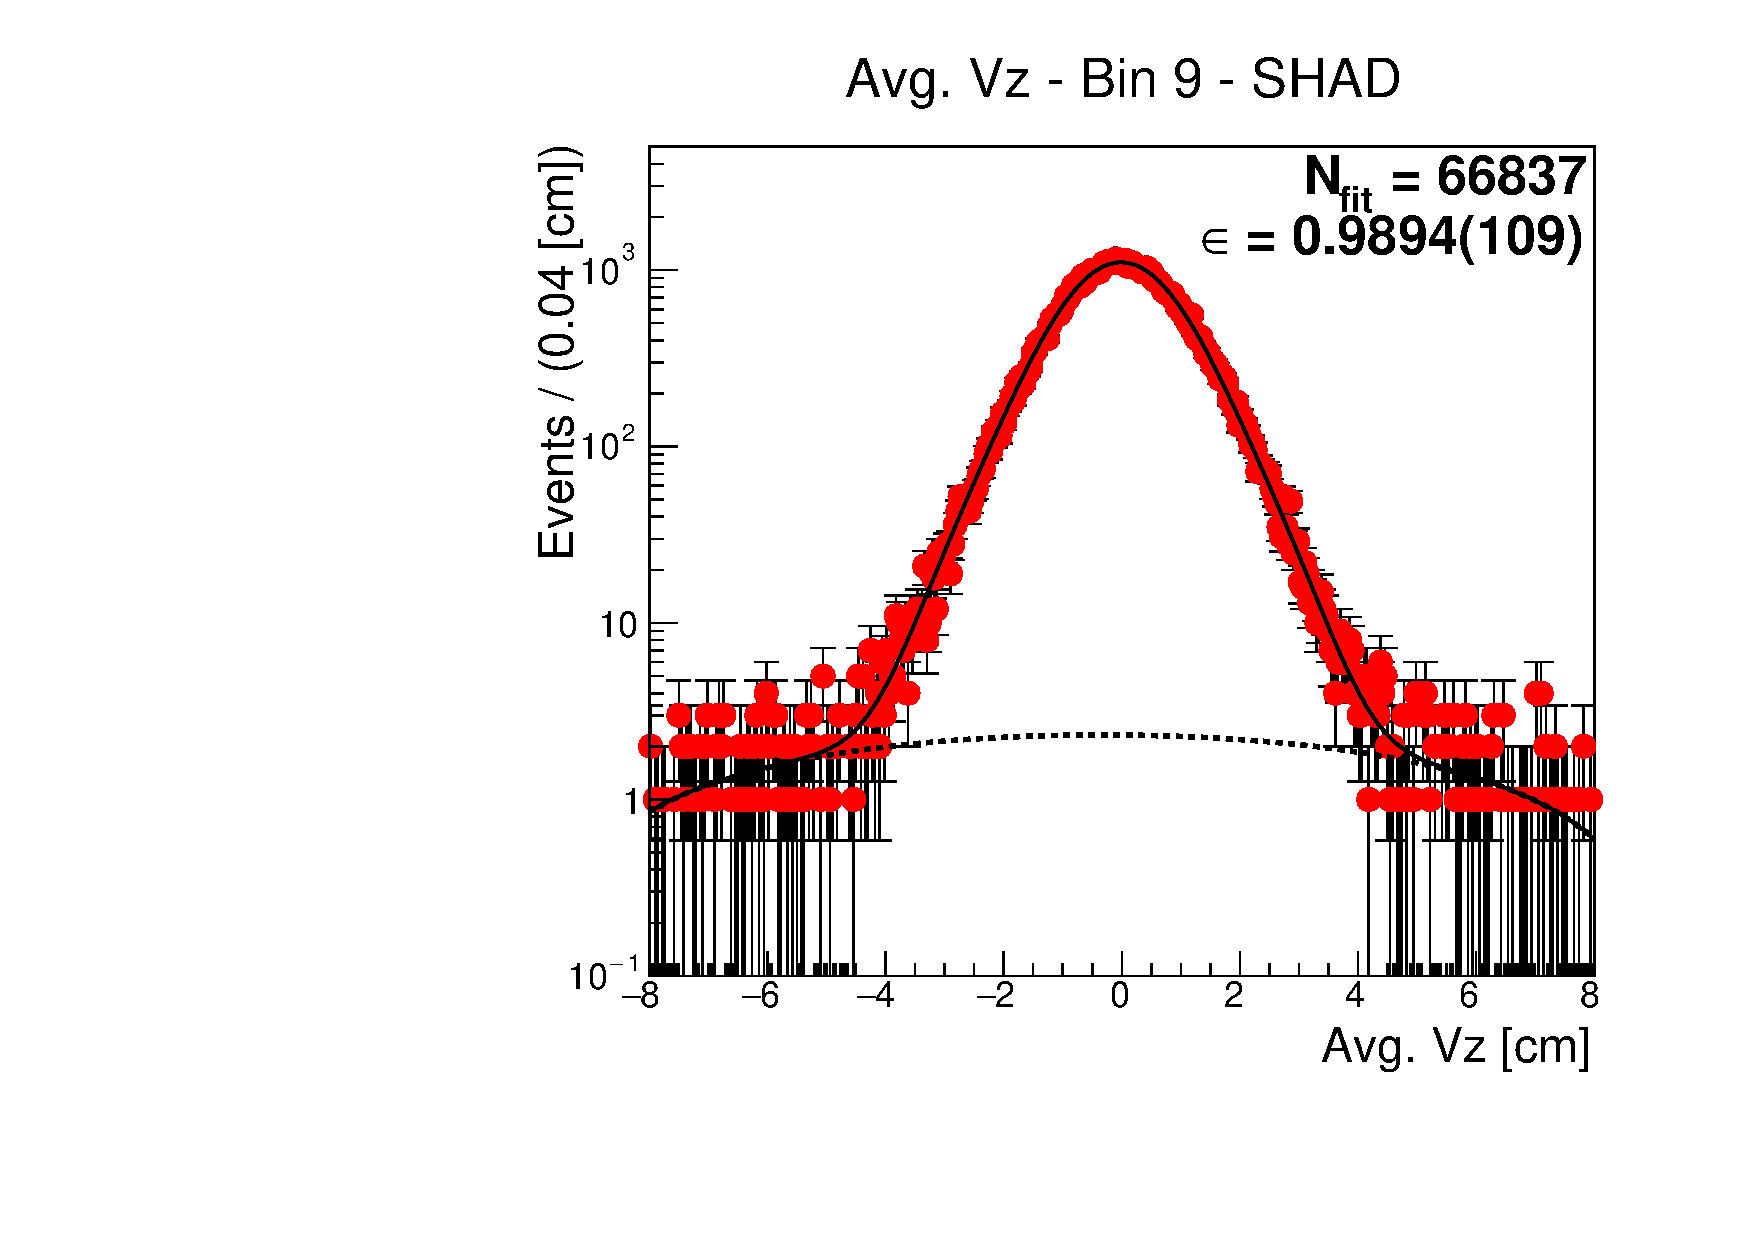
\includegraphics[scale=0.25]{figures/plots/nonDDbar_fit_results/scan/fit_scan_09_data_SHAD.pdf}
\hspace{-0.5cm}
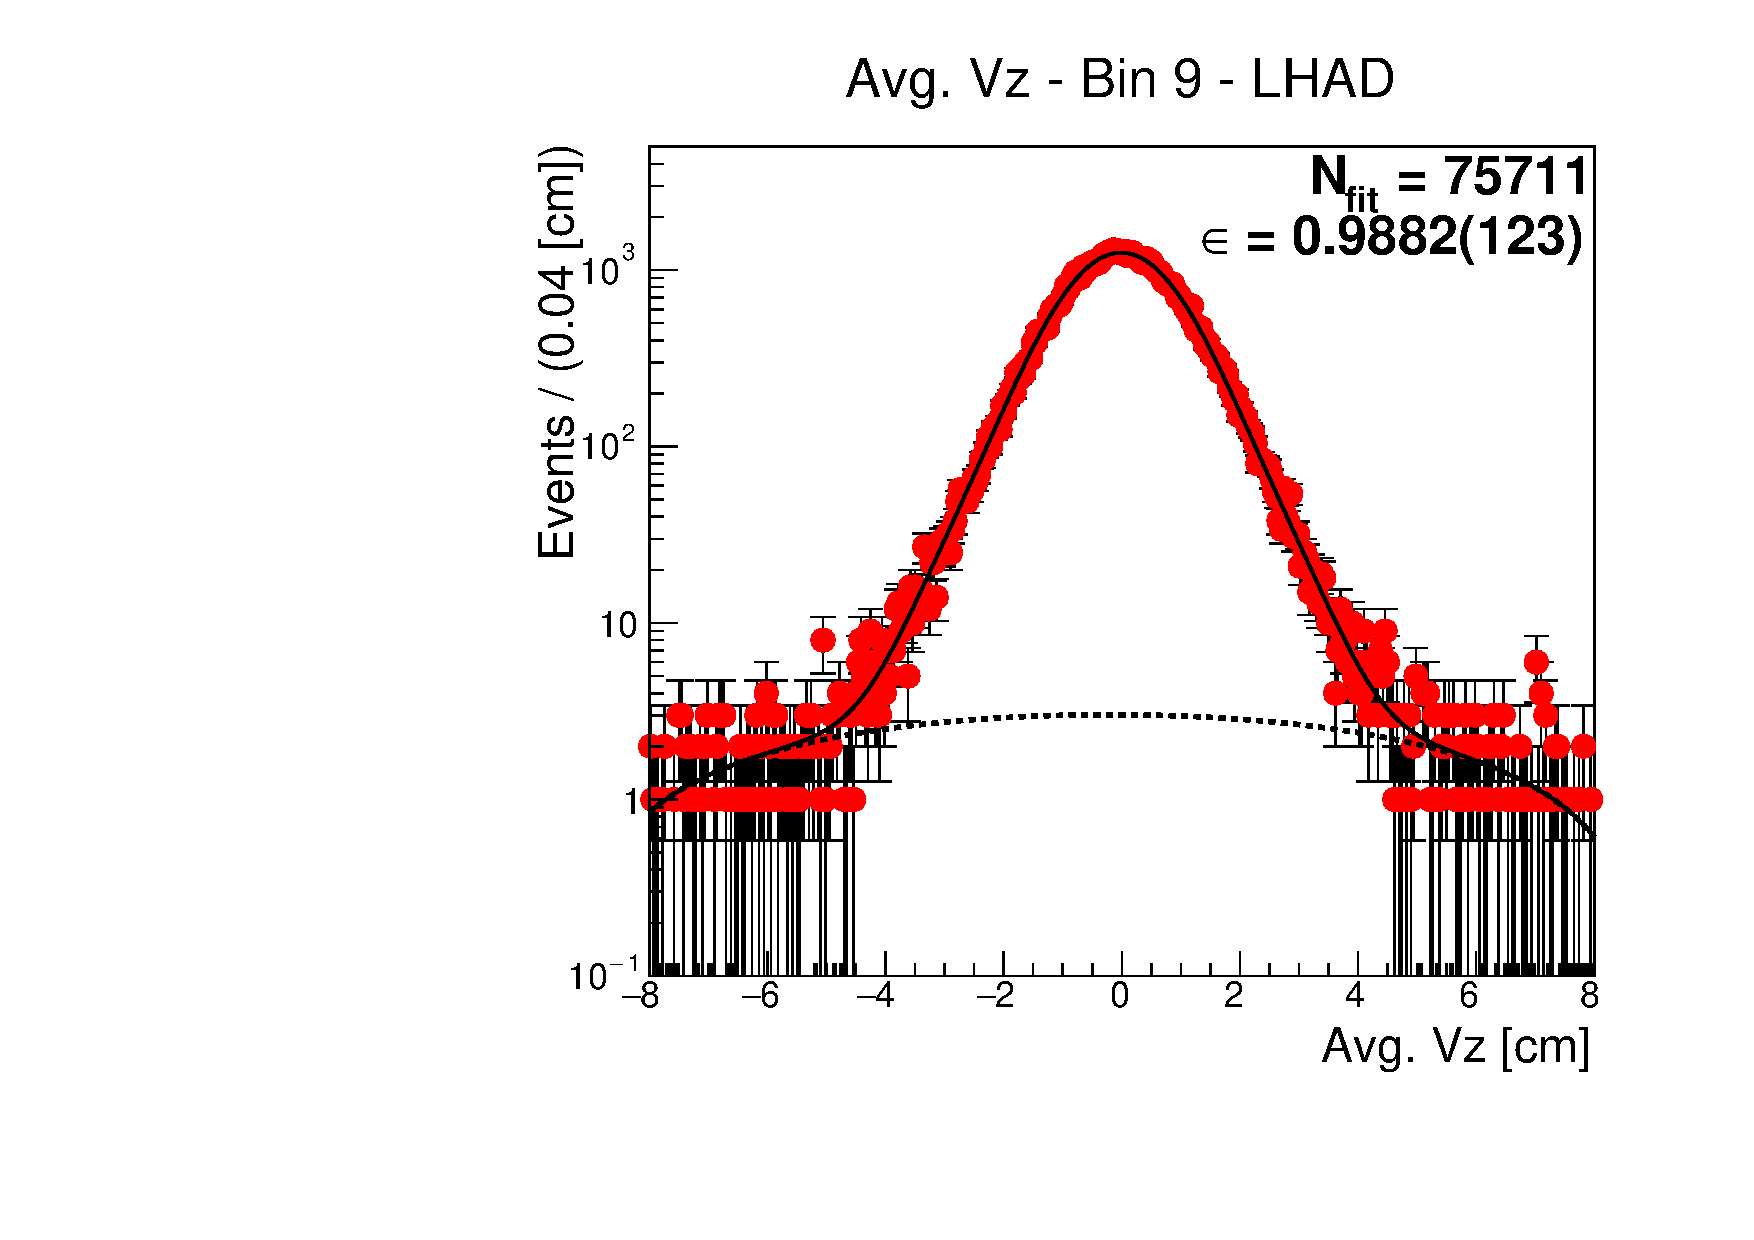
\includegraphics[scale=0.25]{figures/plots/nonDDbar_fit_results/scan/fit_scan_09_data_LHAD.pdf}
\hspace{-0.5cm}
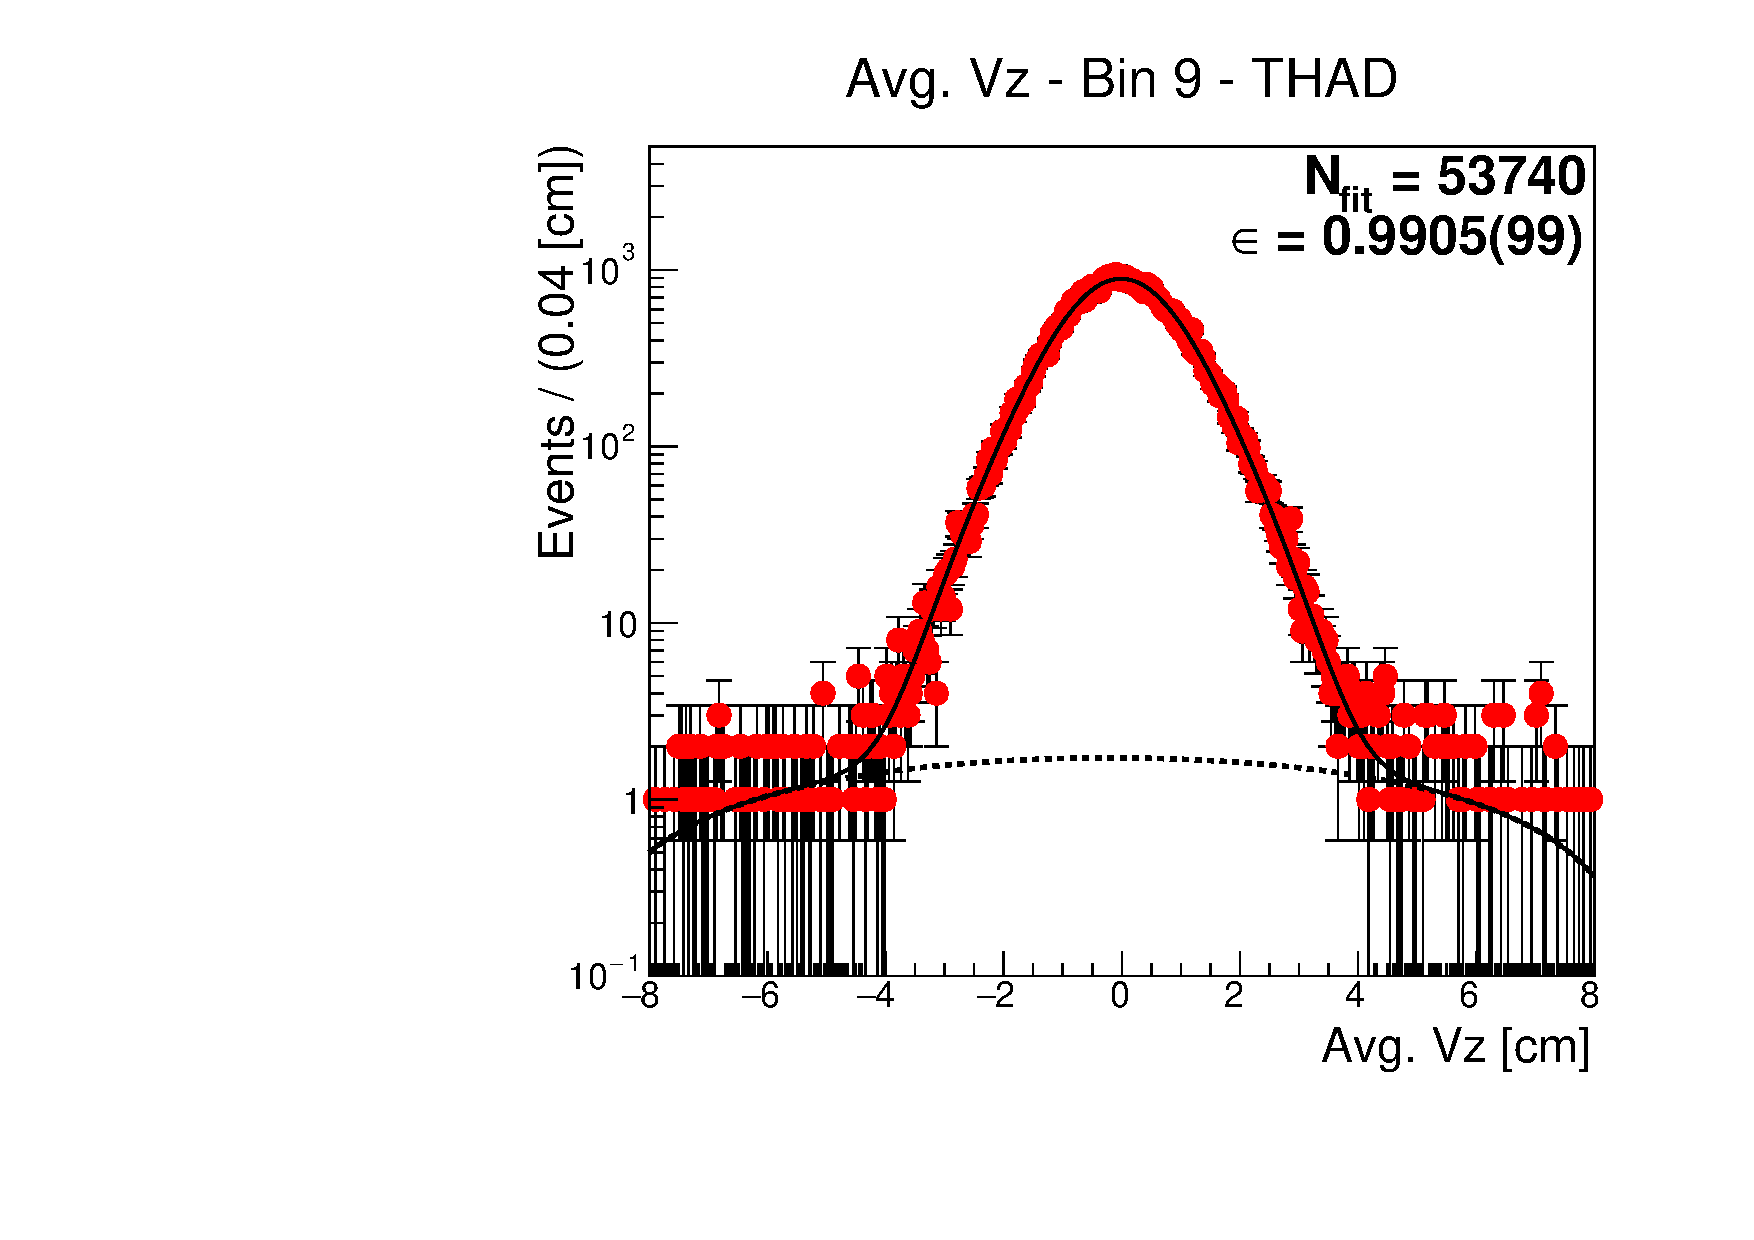
\includegraphics[scale=0.25]{figures/plots/nonDDbar_fit_results/scan/fit_scan_09_data_THAD.pdf}
\caption{Fits to determine the number of hadrons in the 3759 (Scan) data sample.}
{This includes results for SHAD (left), LHAD (middle), and THAD (right).}
\label{fig:hadron_fits_scan_09}
\end{figure}

\begin{figure}[H]
\centering
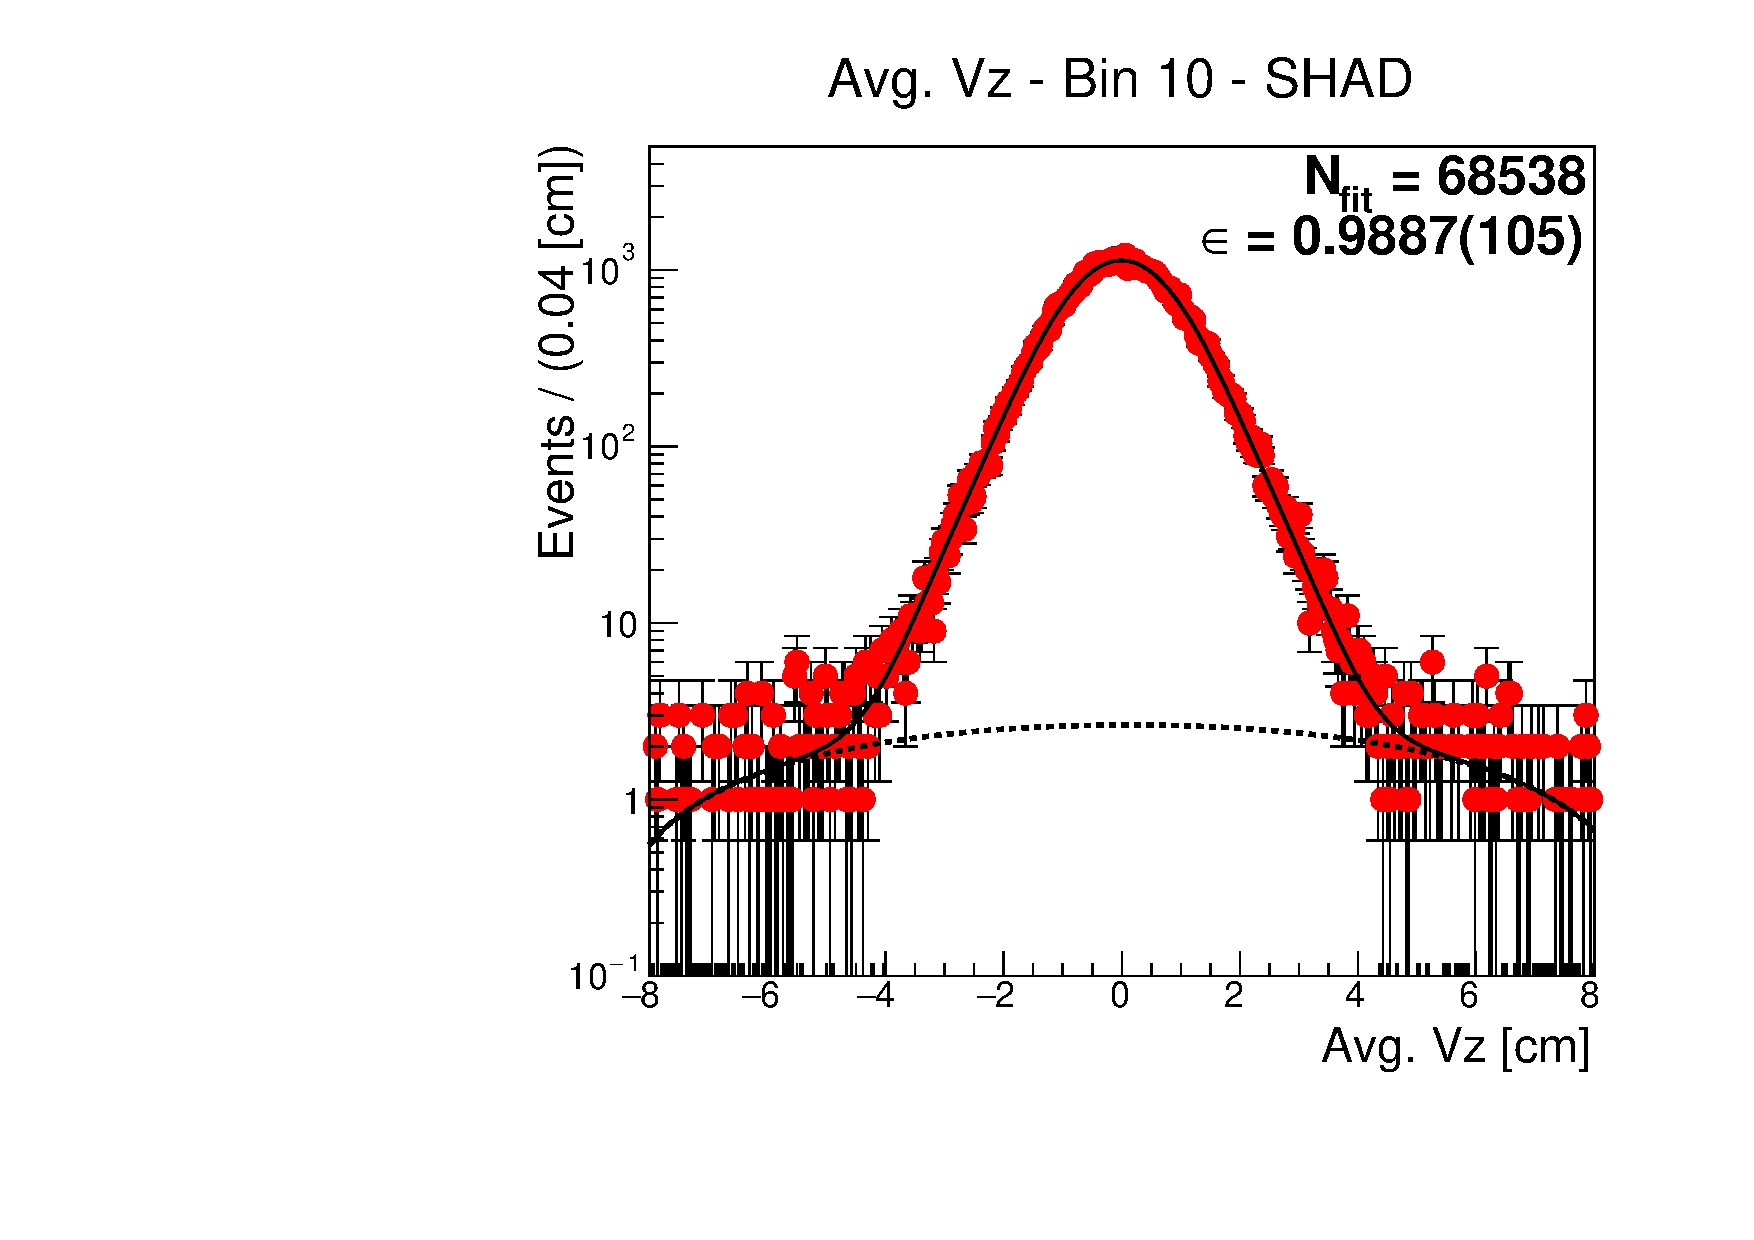
\includegraphics[scale=0.25]{figures/plots/nonDDbar_fit_results/scan/fit_scan_10_data_SHAD.pdf}
\hspace{-0.5cm}
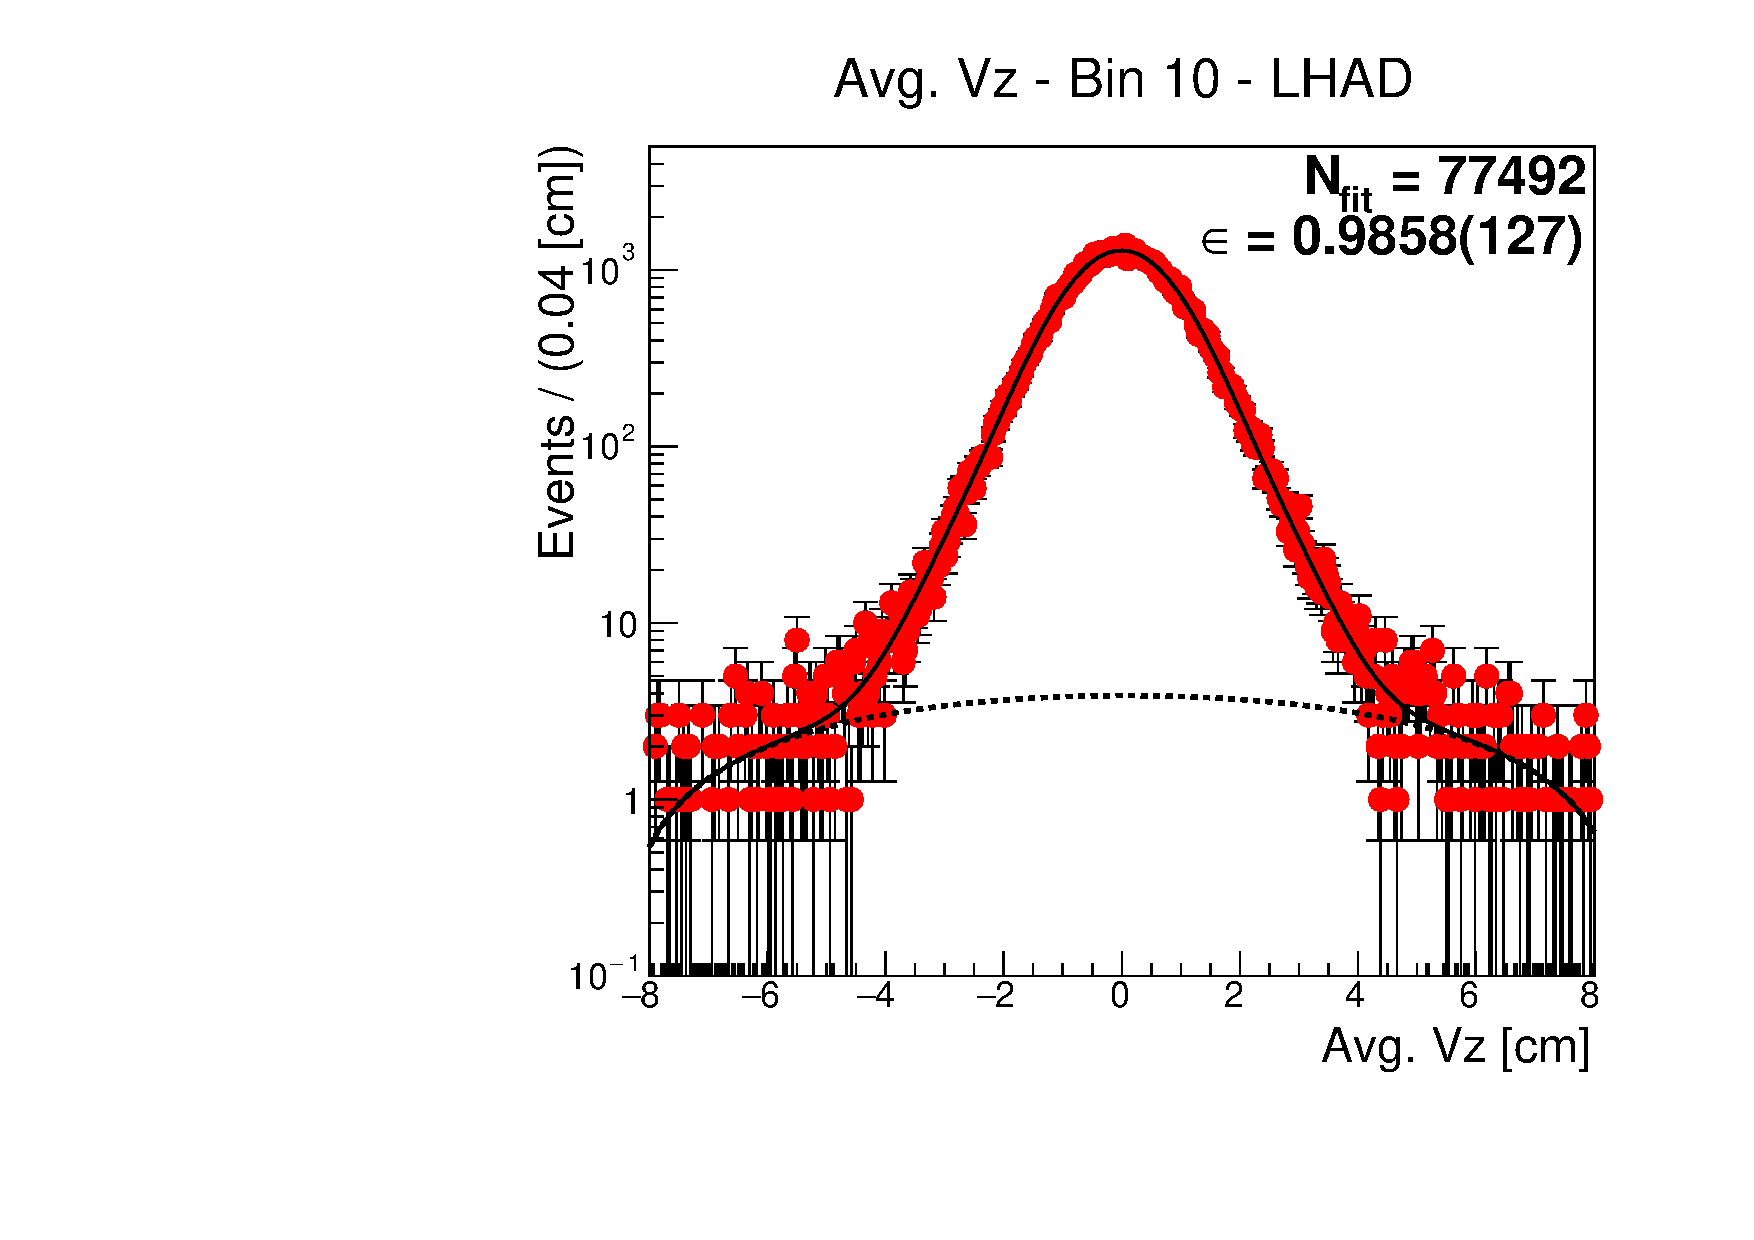
\includegraphics[scale=0.25]{figures/plots/nonDDbar_fit_results/scan/fit_scan_10_data_LHAD.pdf}
\hspace{-0.5cm}
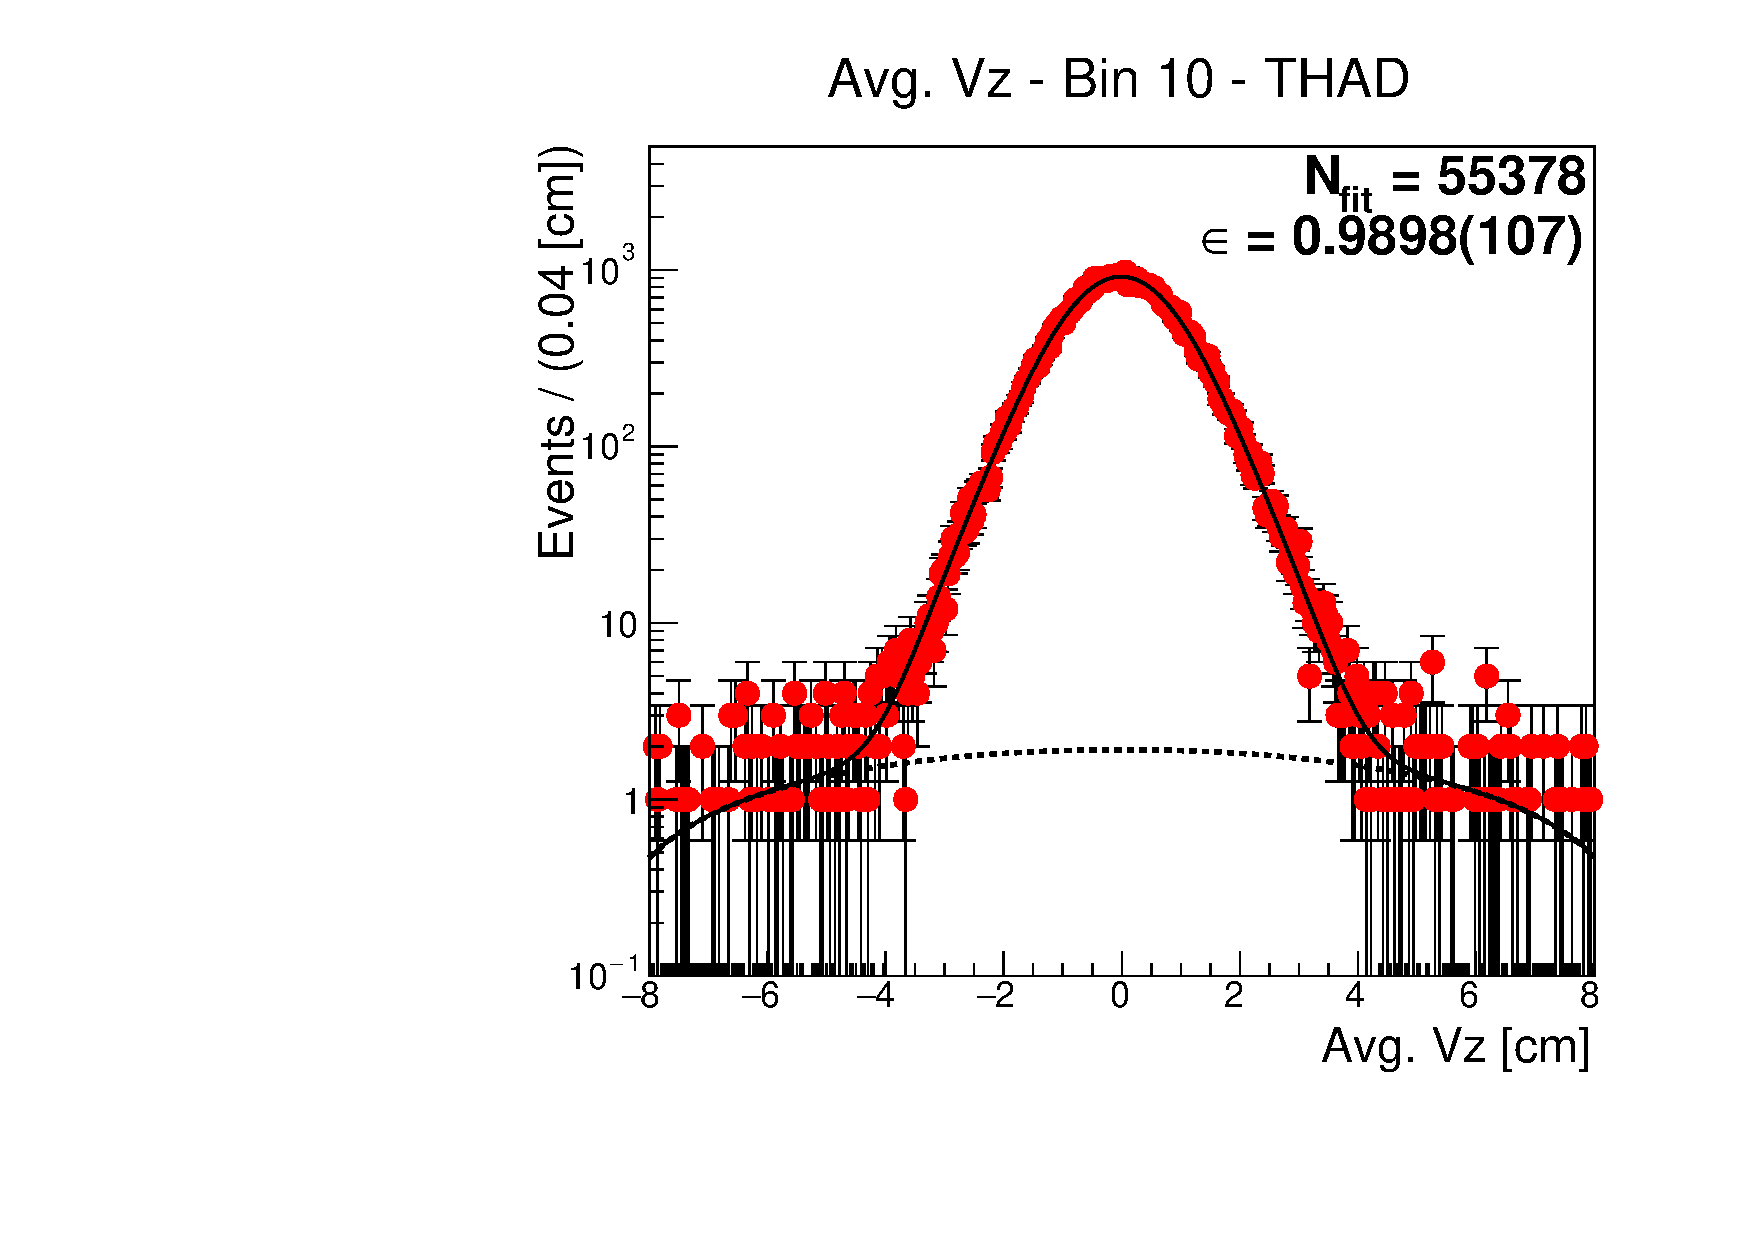
\includegraphics[scale=0.25]{figures/plots/nonDDbar_fit_results/scan/fit_scan_10_data_THAD.pdf}
\caption{Fits to determine the number of hadrons in the 3762 (Scan) data sample.}
{This includes results for SHAD (left), LHAD (middle), and THAD (right).}
\label{fig:hadron_fits_scan_10}
\end{figure}

\begin{figure}[H]
\centering
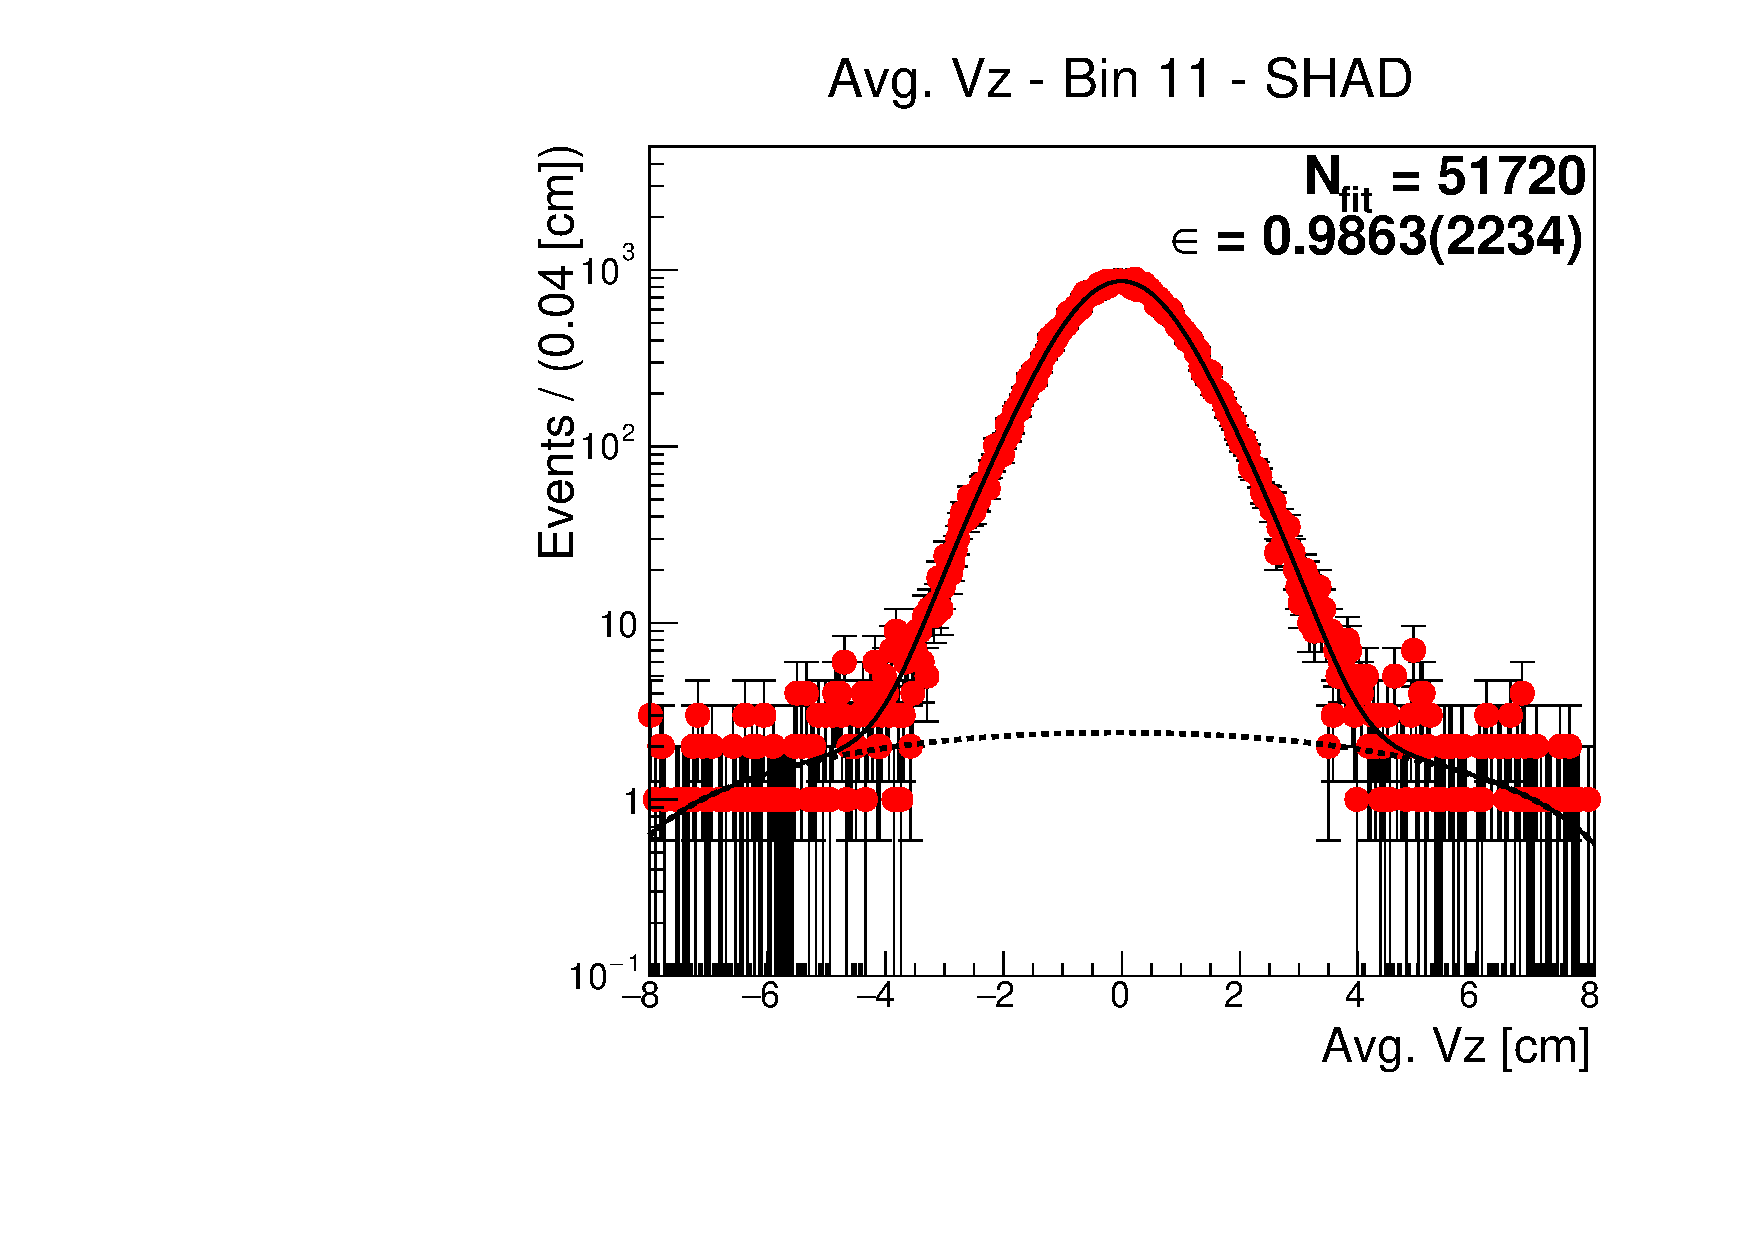
\includegraphics[scale=0.25]{figures/plots/nonDDbar_fit_results/scan/fit_scan_11_data_SHAD.pdf}
\hspace{-0.5cm}
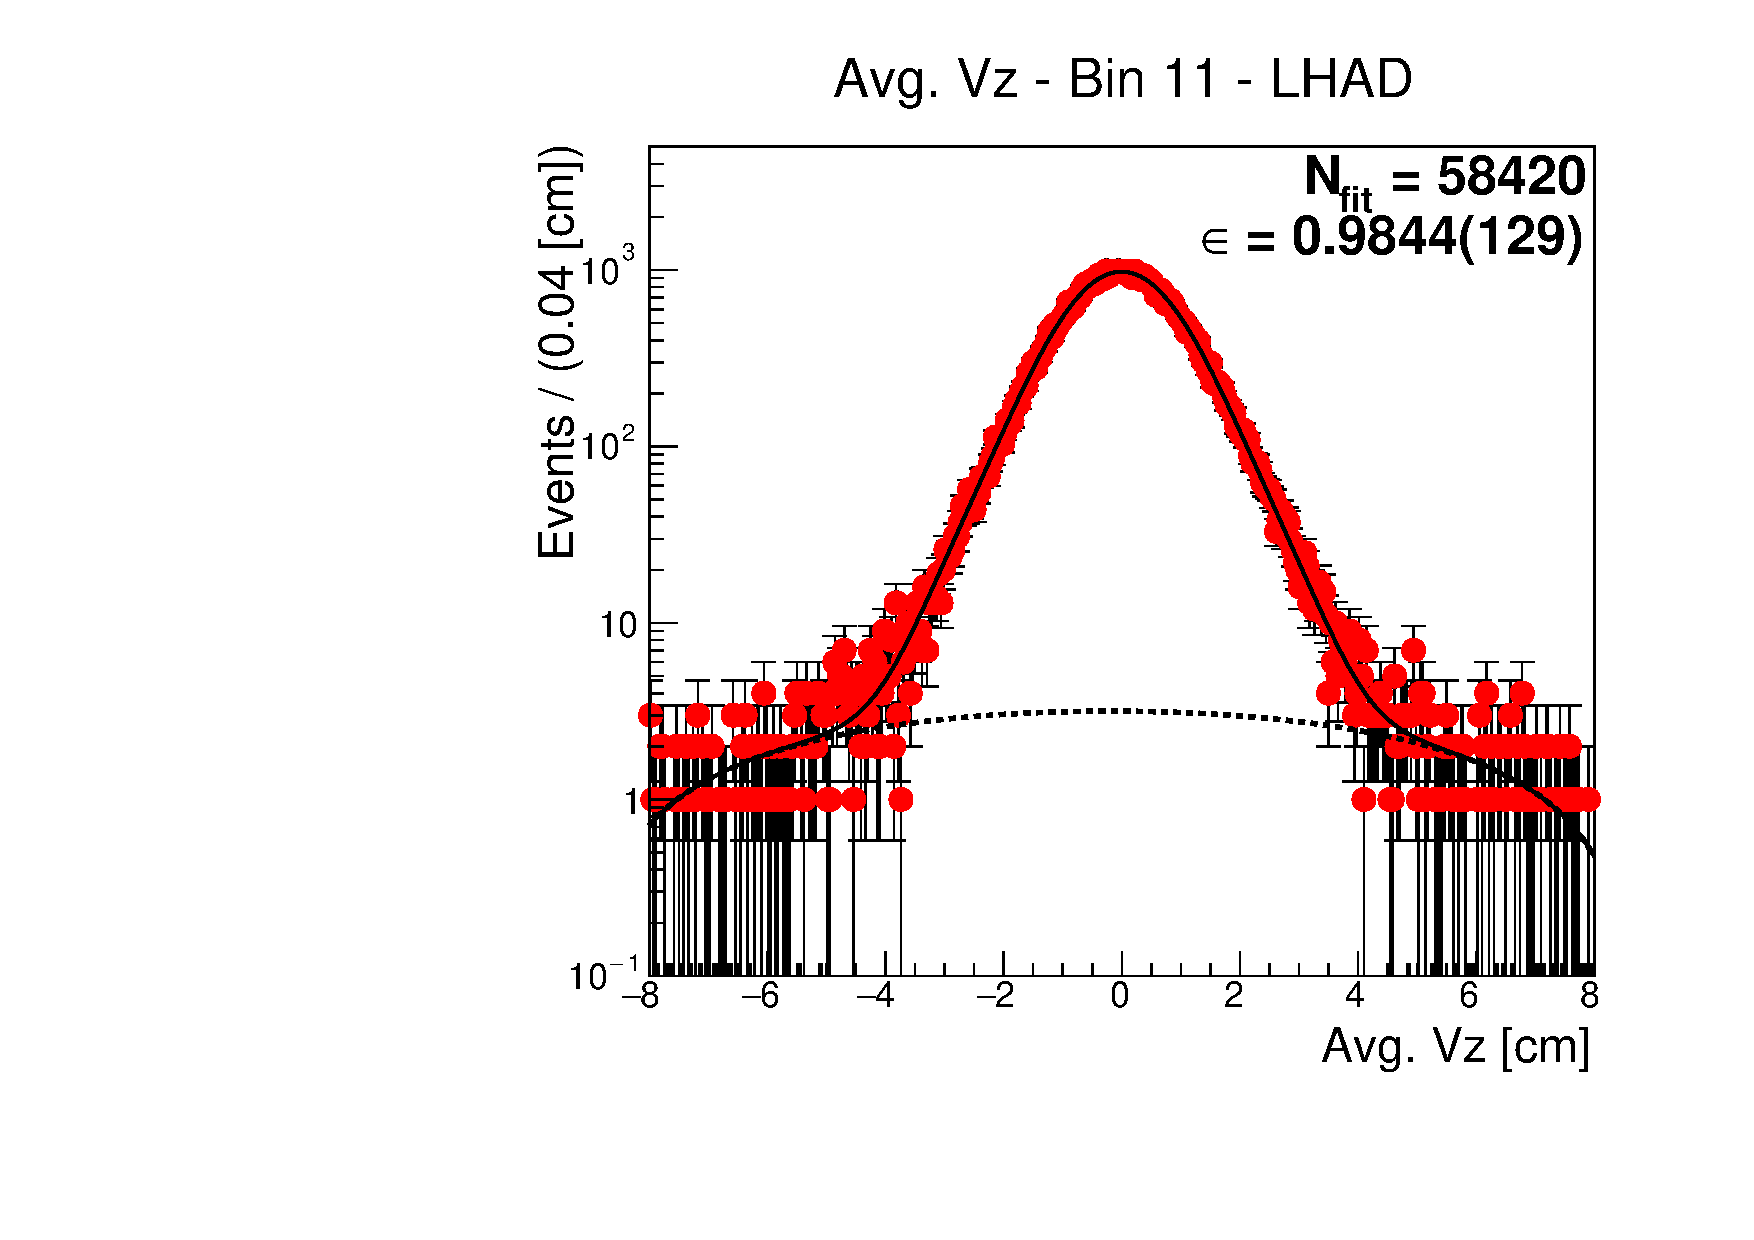
\includegraphics[scale=0.25]{figures/plots/nonDDbar_fit_results/scan/fit_scan_11_data_LHAD.pdf}
\hspace{-0.5cm}
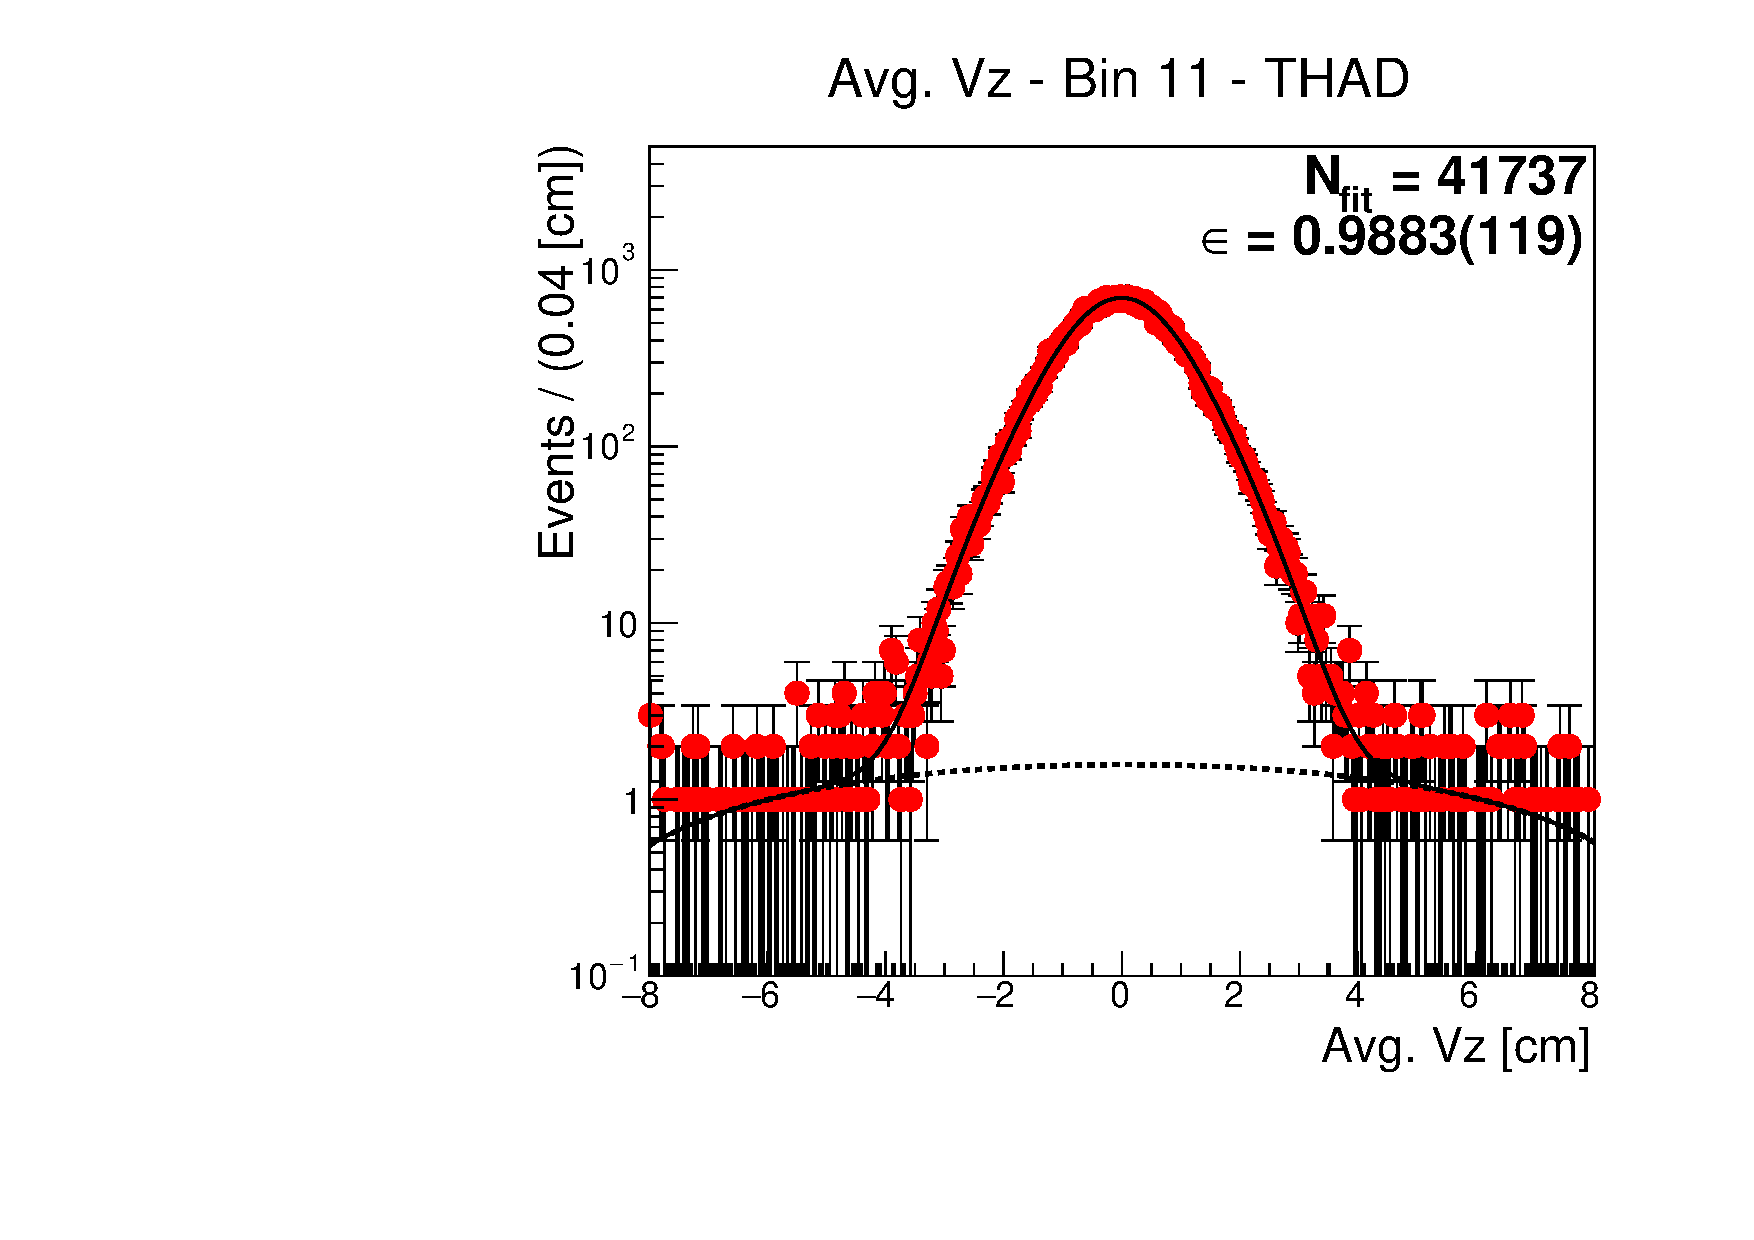
\includegraphics[scale=0.25]{figures/plots/nonDDbar_fit_results/scan/fit_scan_11_data_THAD.pdf}
\caption{Fits to determine the number of hadrons in the 3765 (Scan) data sample.}
{This includes results for SHAD (left), LHAD (middle), and THAD (right).}
\label{fig:hadron_fits_scan_11}
\end{figure}

\begin{figure}[H]
\centering
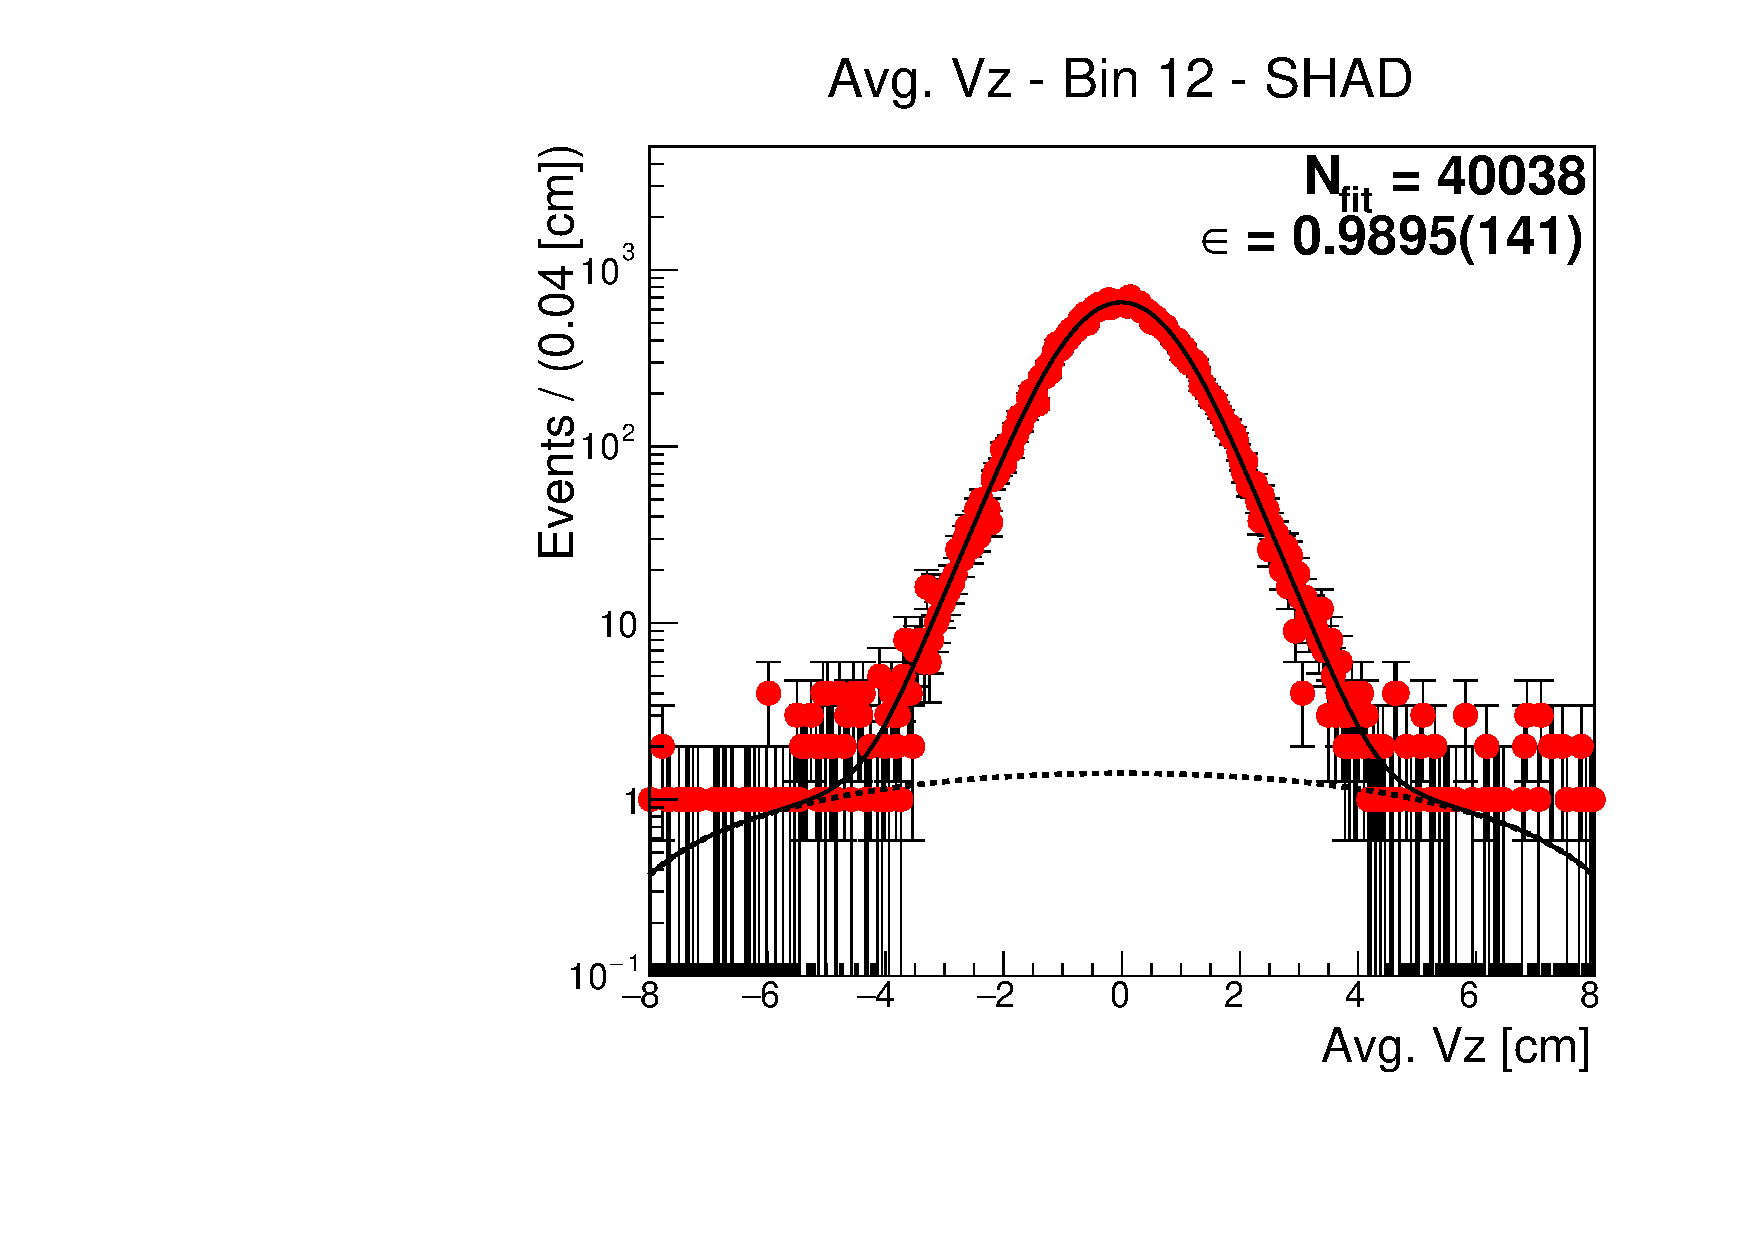
\includegraphics[scale=0.25]{figures/plots/nonDDbar_fit_results/scan/fit_scan_12_data_SHAD.pdf}
\hspace{-0.5cm}
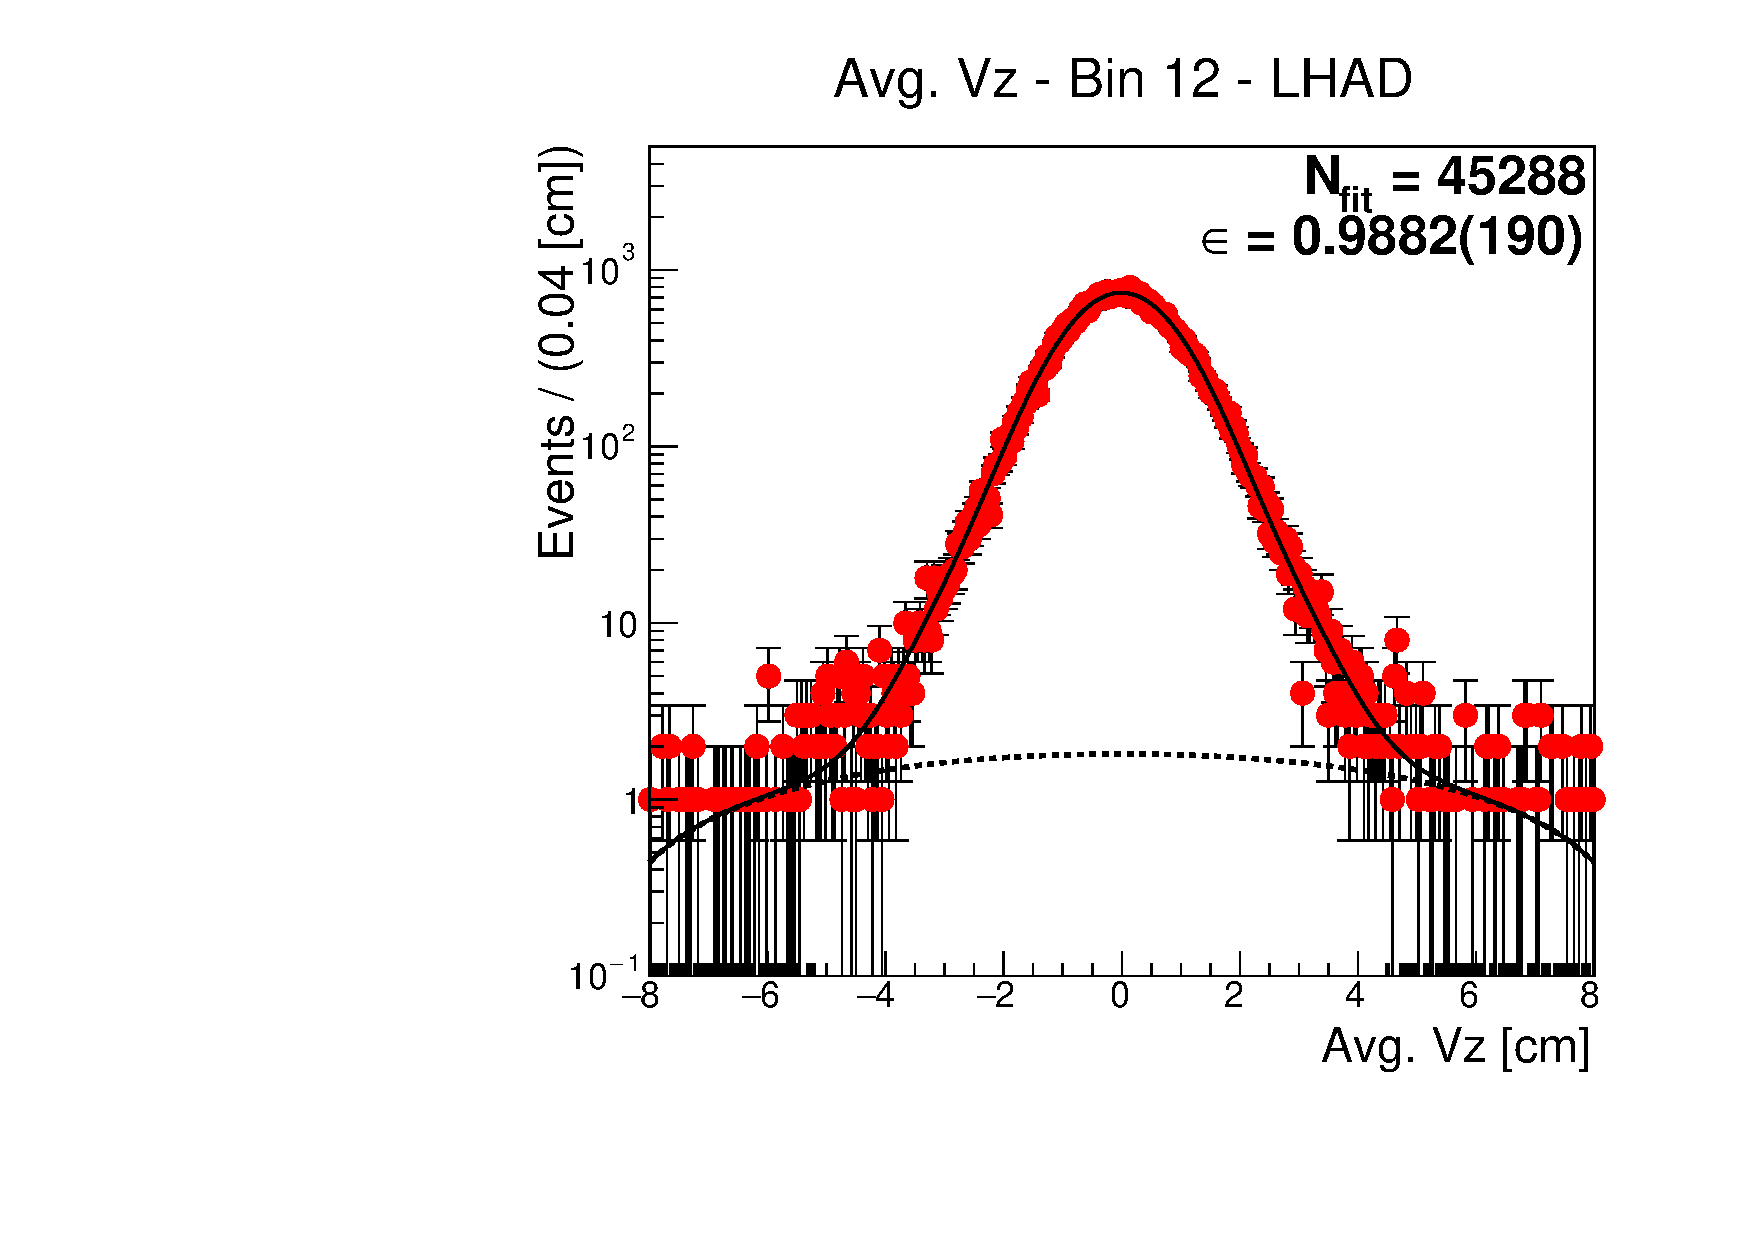
\includegraphics[scale=0.25]{figures/plots/nonDDbar_fit_results/scan/fit_scan_12_data_LHAD.pdf}
\hspace{-0.5cm}
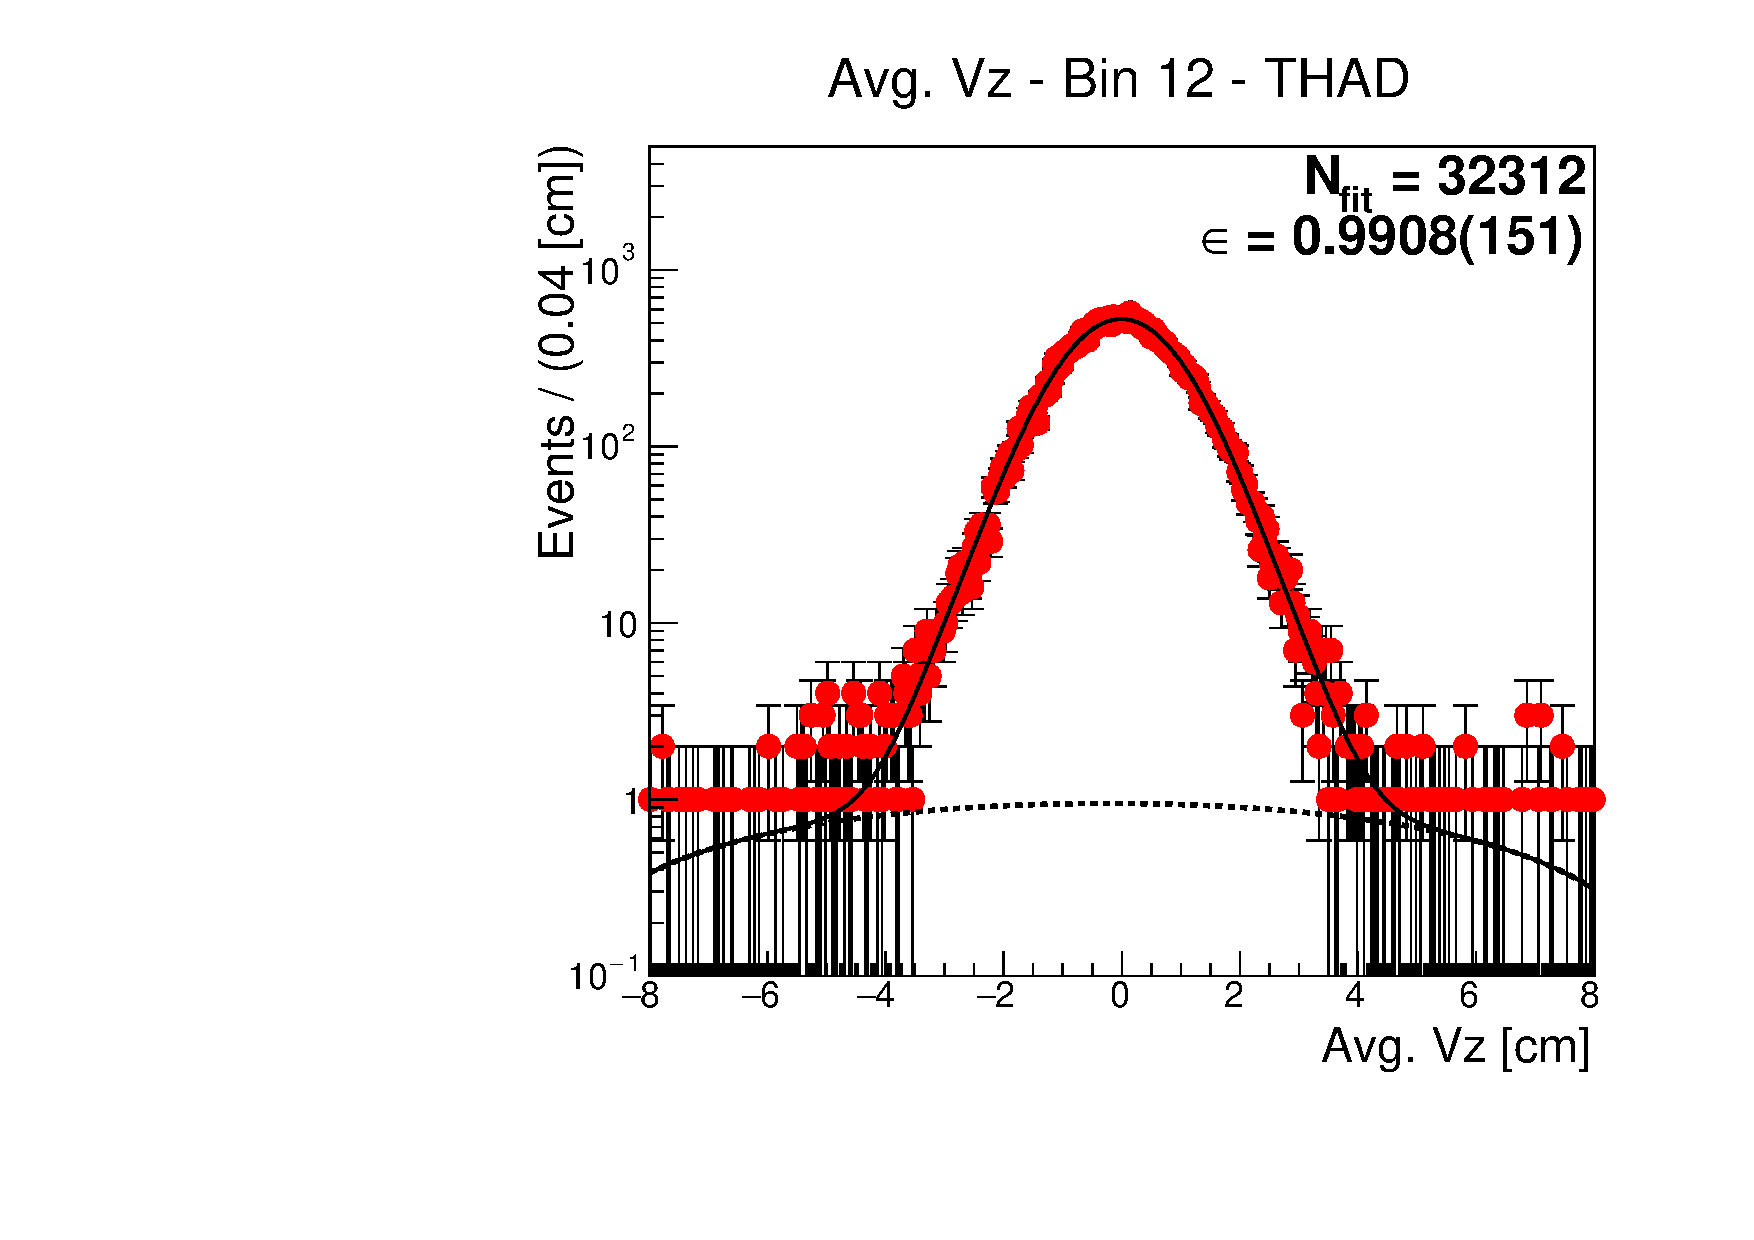
\includegraphics[scale=0.25]{figures/plots/nonDDbar_fit_results/scan/fit_scan_12_data_THAD.pdf}
\caption{Fits to determine the number of hadrons in the 3767 (Scan) data sample.}
{This includes results for SHAD (left), LHAD (middle), and THAD (right).}
\label{fig:hadron_fits_scan_12}
\end{figure}

\begin{figure}[H]
\centering
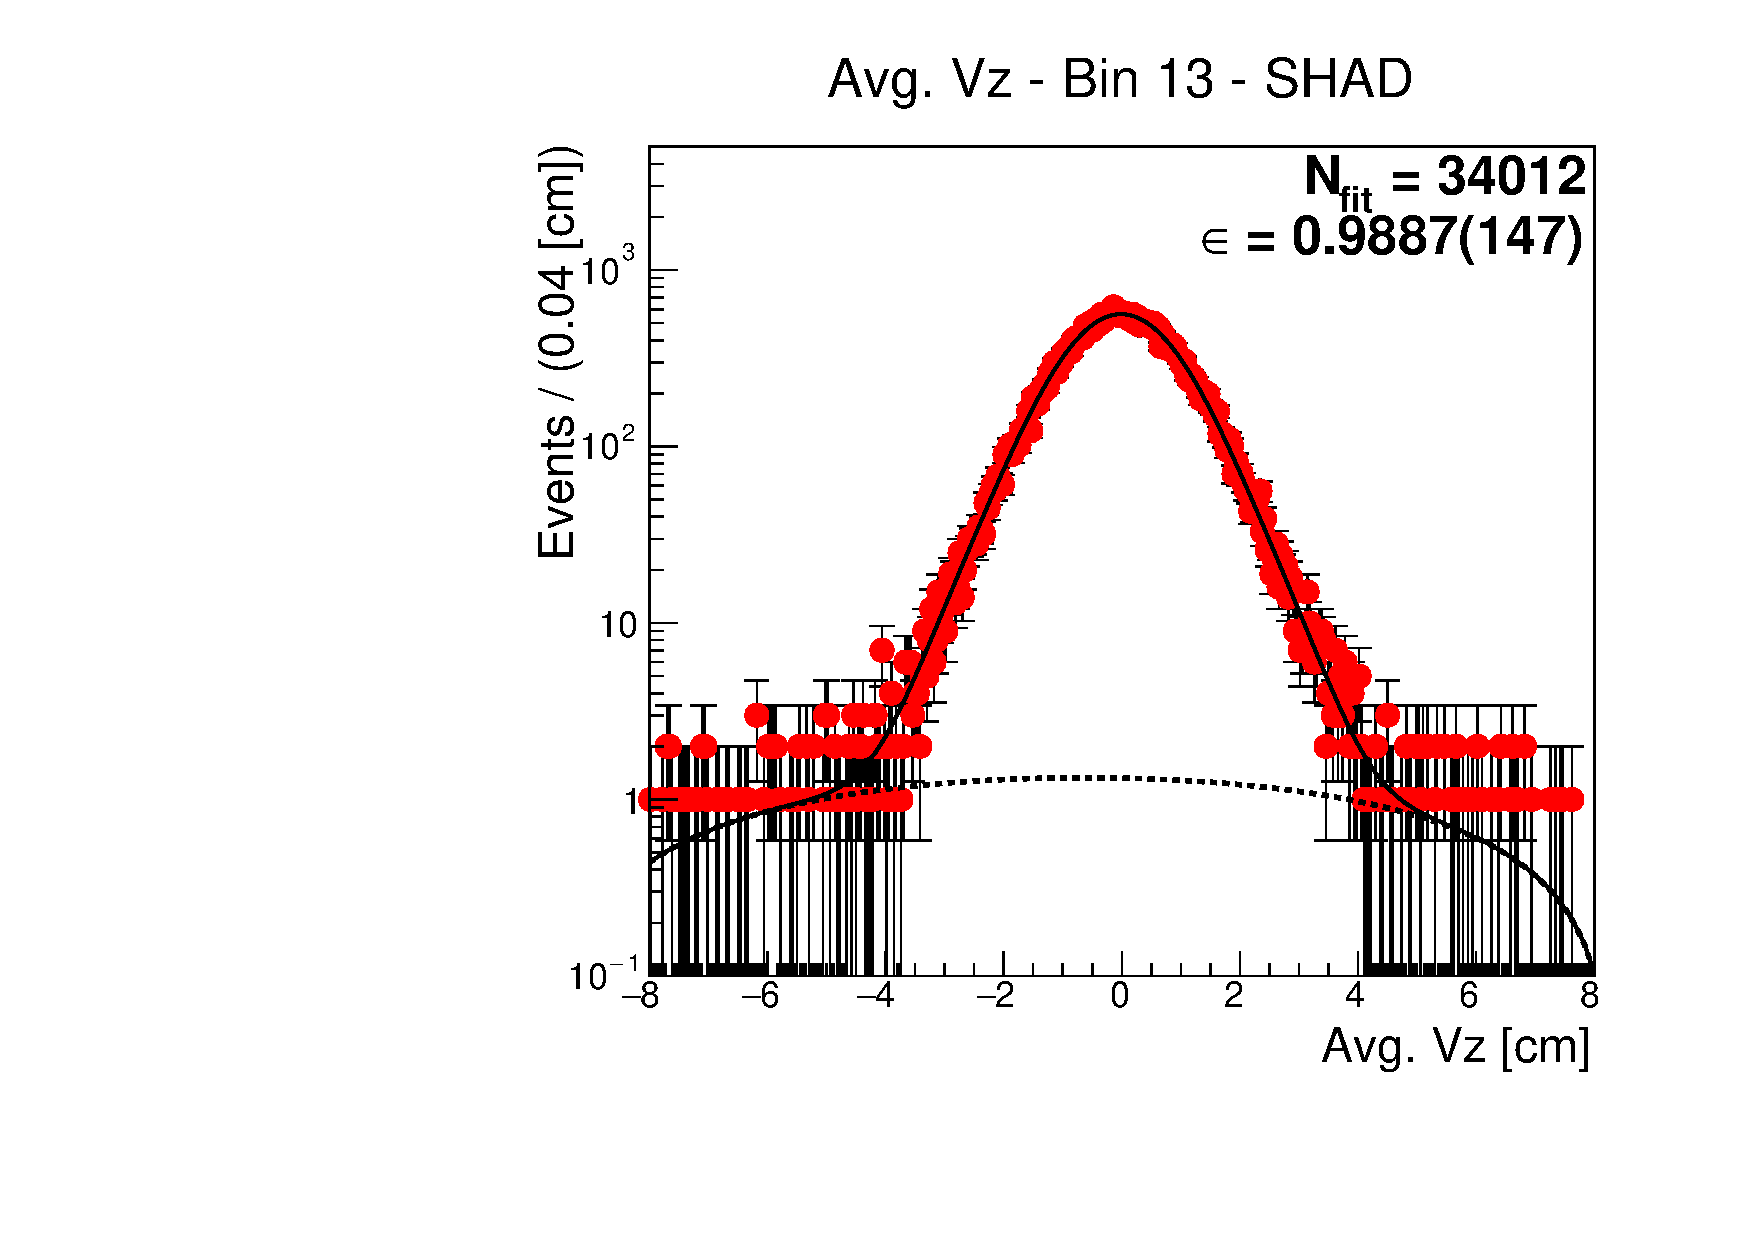
\includegraphics[scale=0.25]{figures/plots/nonDDbar_fit_results/scan/fit_scan_13_data_SHAD.pdf}
\hspace{-0.5cm}
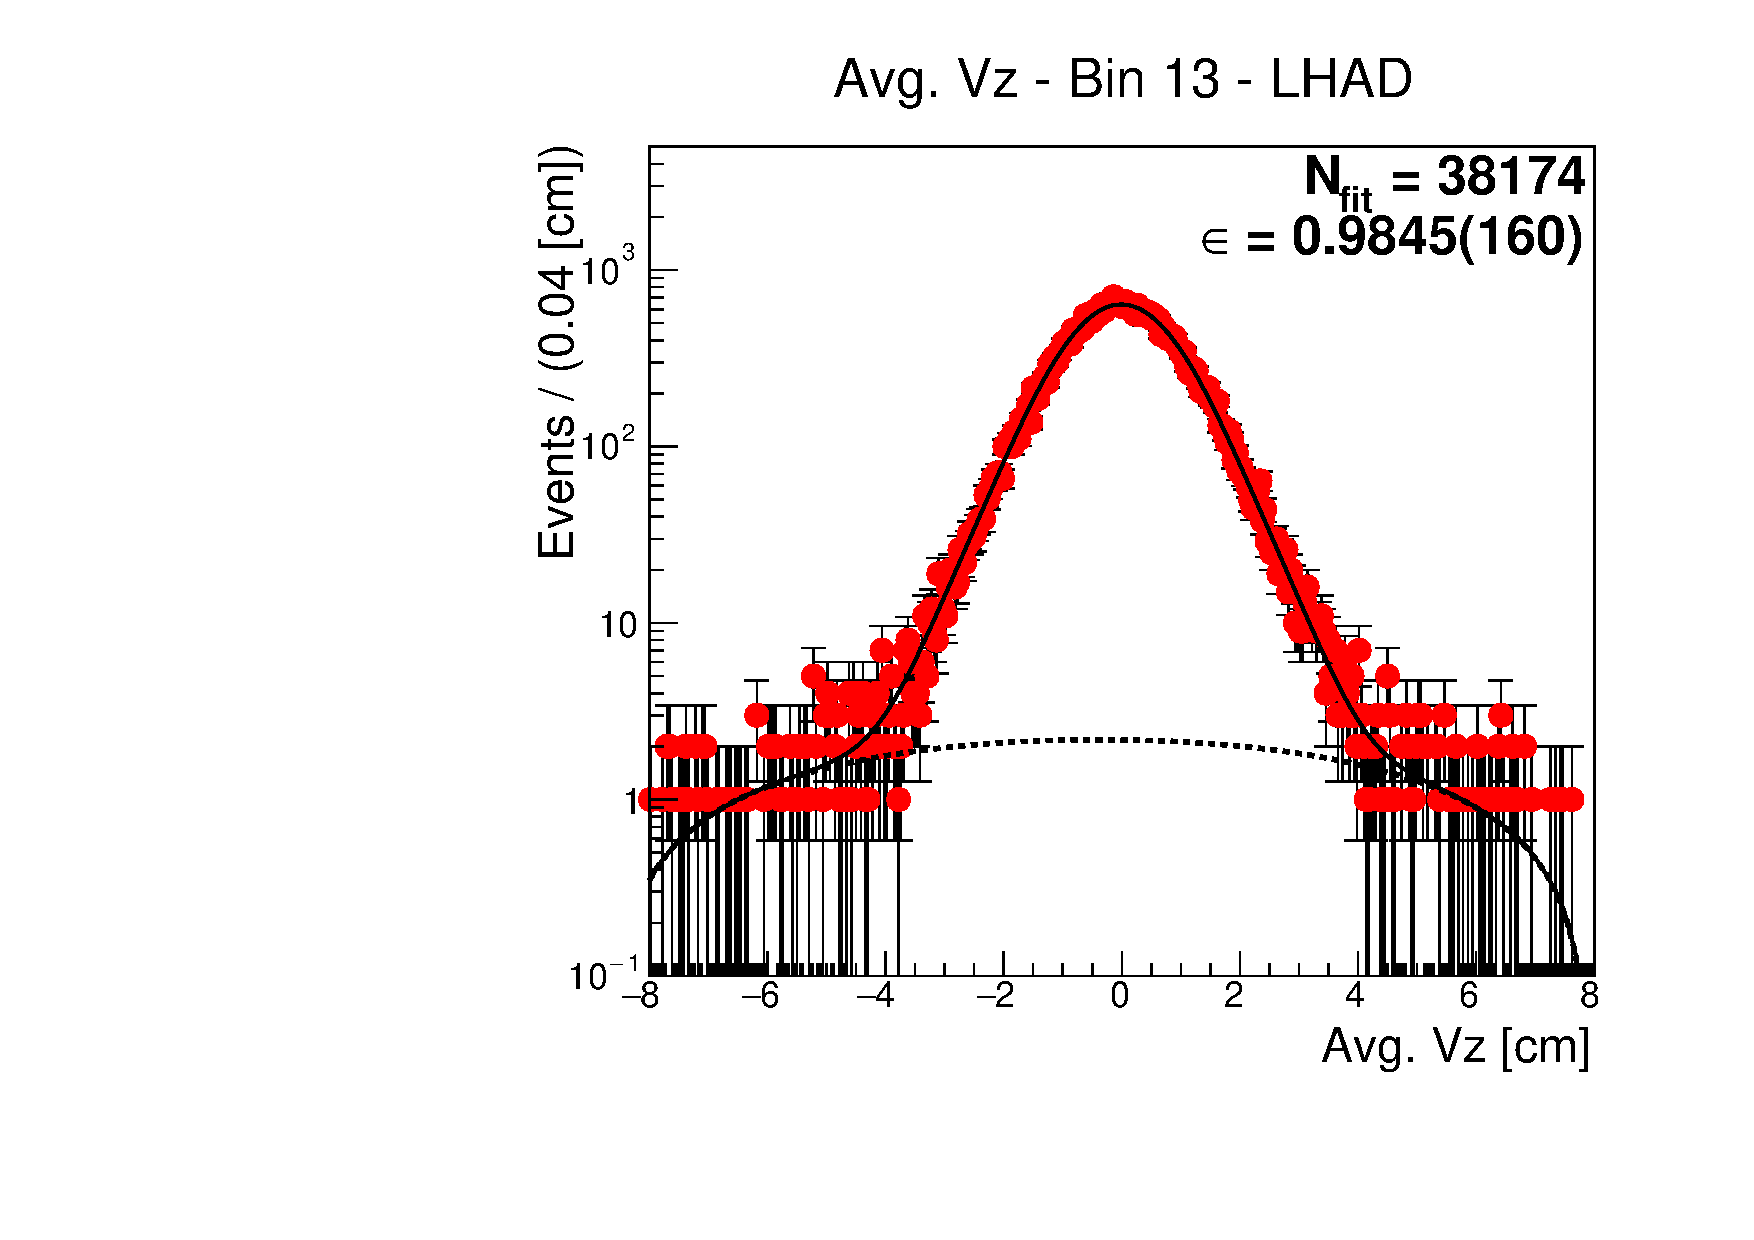
\includegraphics[scale=0.25]{figures/plots/nonDDbar_fit_results/scan/fit_scan_13_data_LHAD.pdf}
\hspace{-0.5cm}
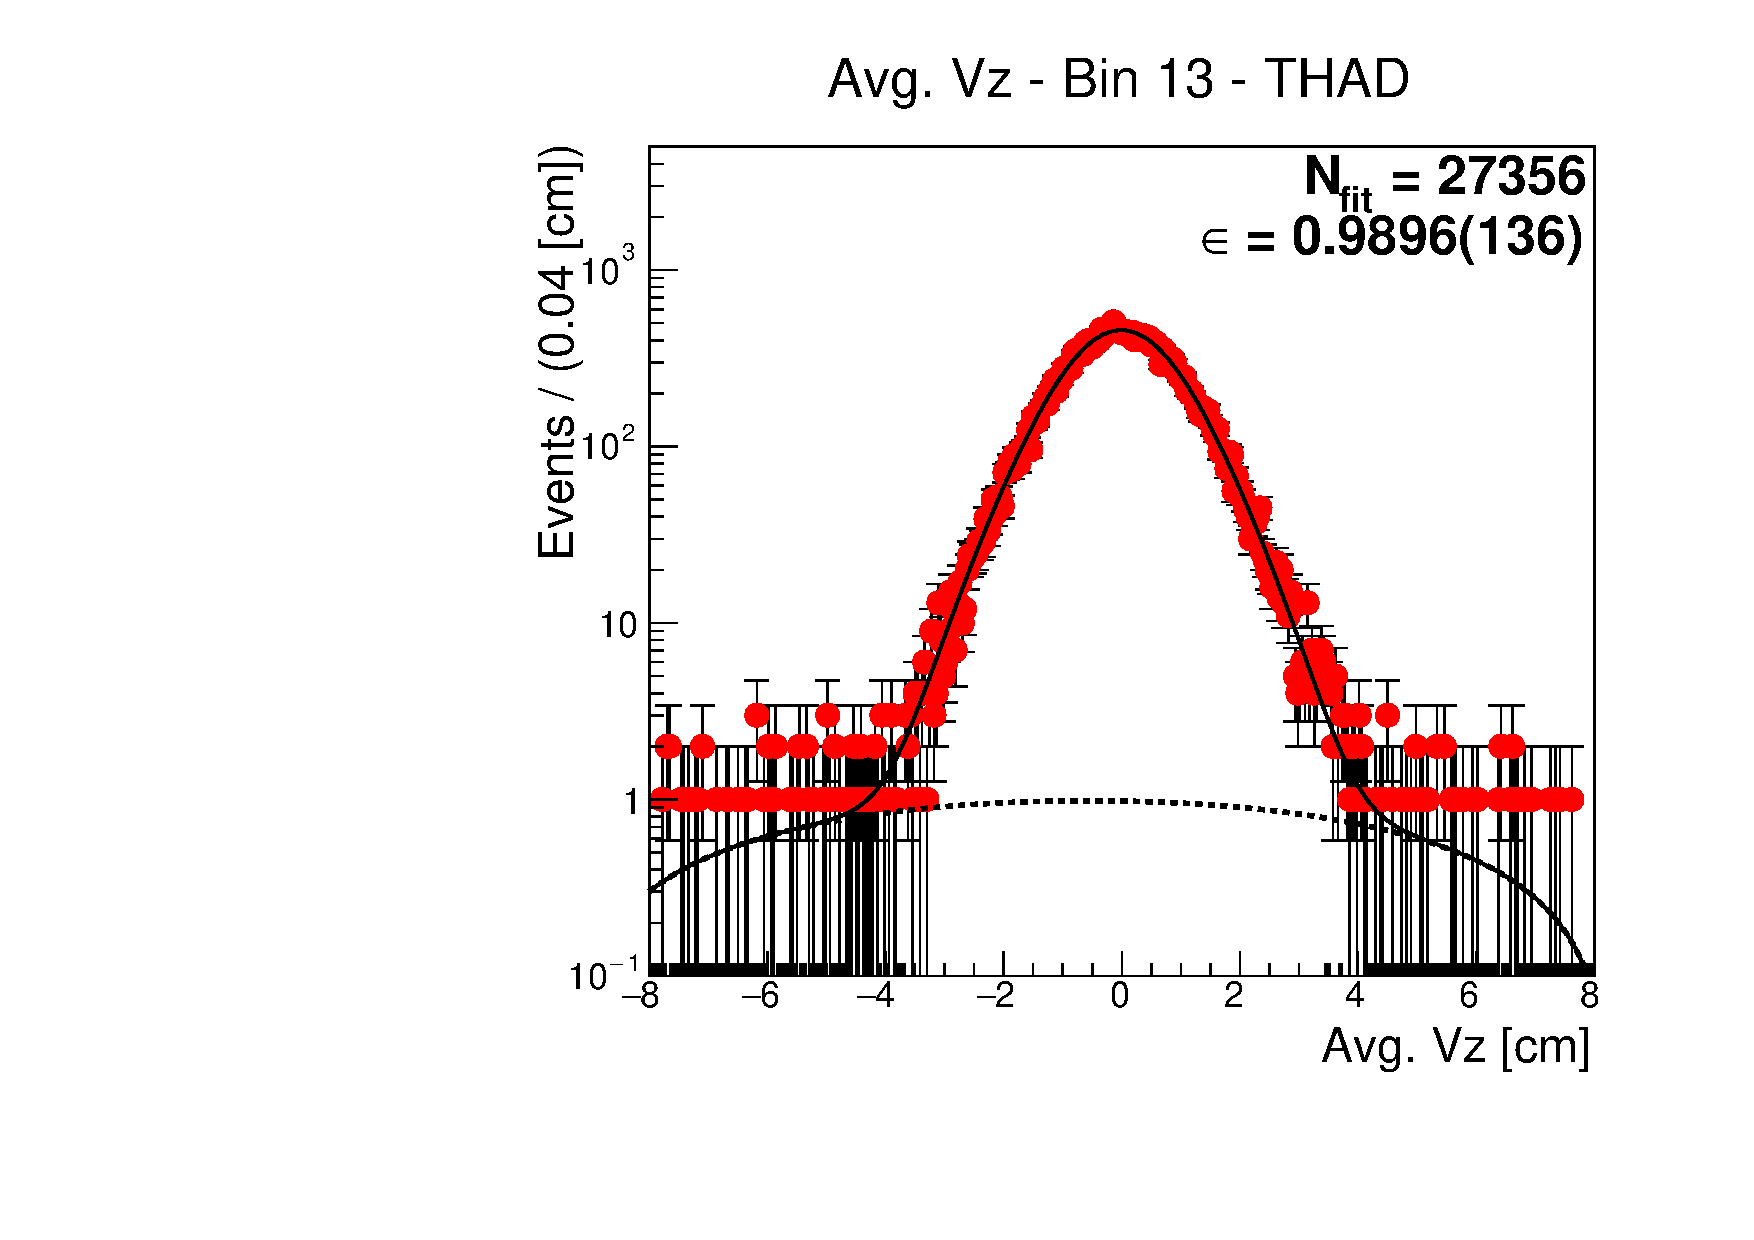
\includegraphics[scale=0.25]{figures/plots/nonDDbar_fit_results/scan/fit_scan_13_data_THAD.pdf}
\caption{Fits to determine the number of hadrons in the 3771 (Scan) data sample.}
{This includes results for SHAD (left), LHAD (middle), and THAD (right).}
\label{fig:hadron_fits_scan_13}
\end{figure}

\begin{figure}[H]
\centering
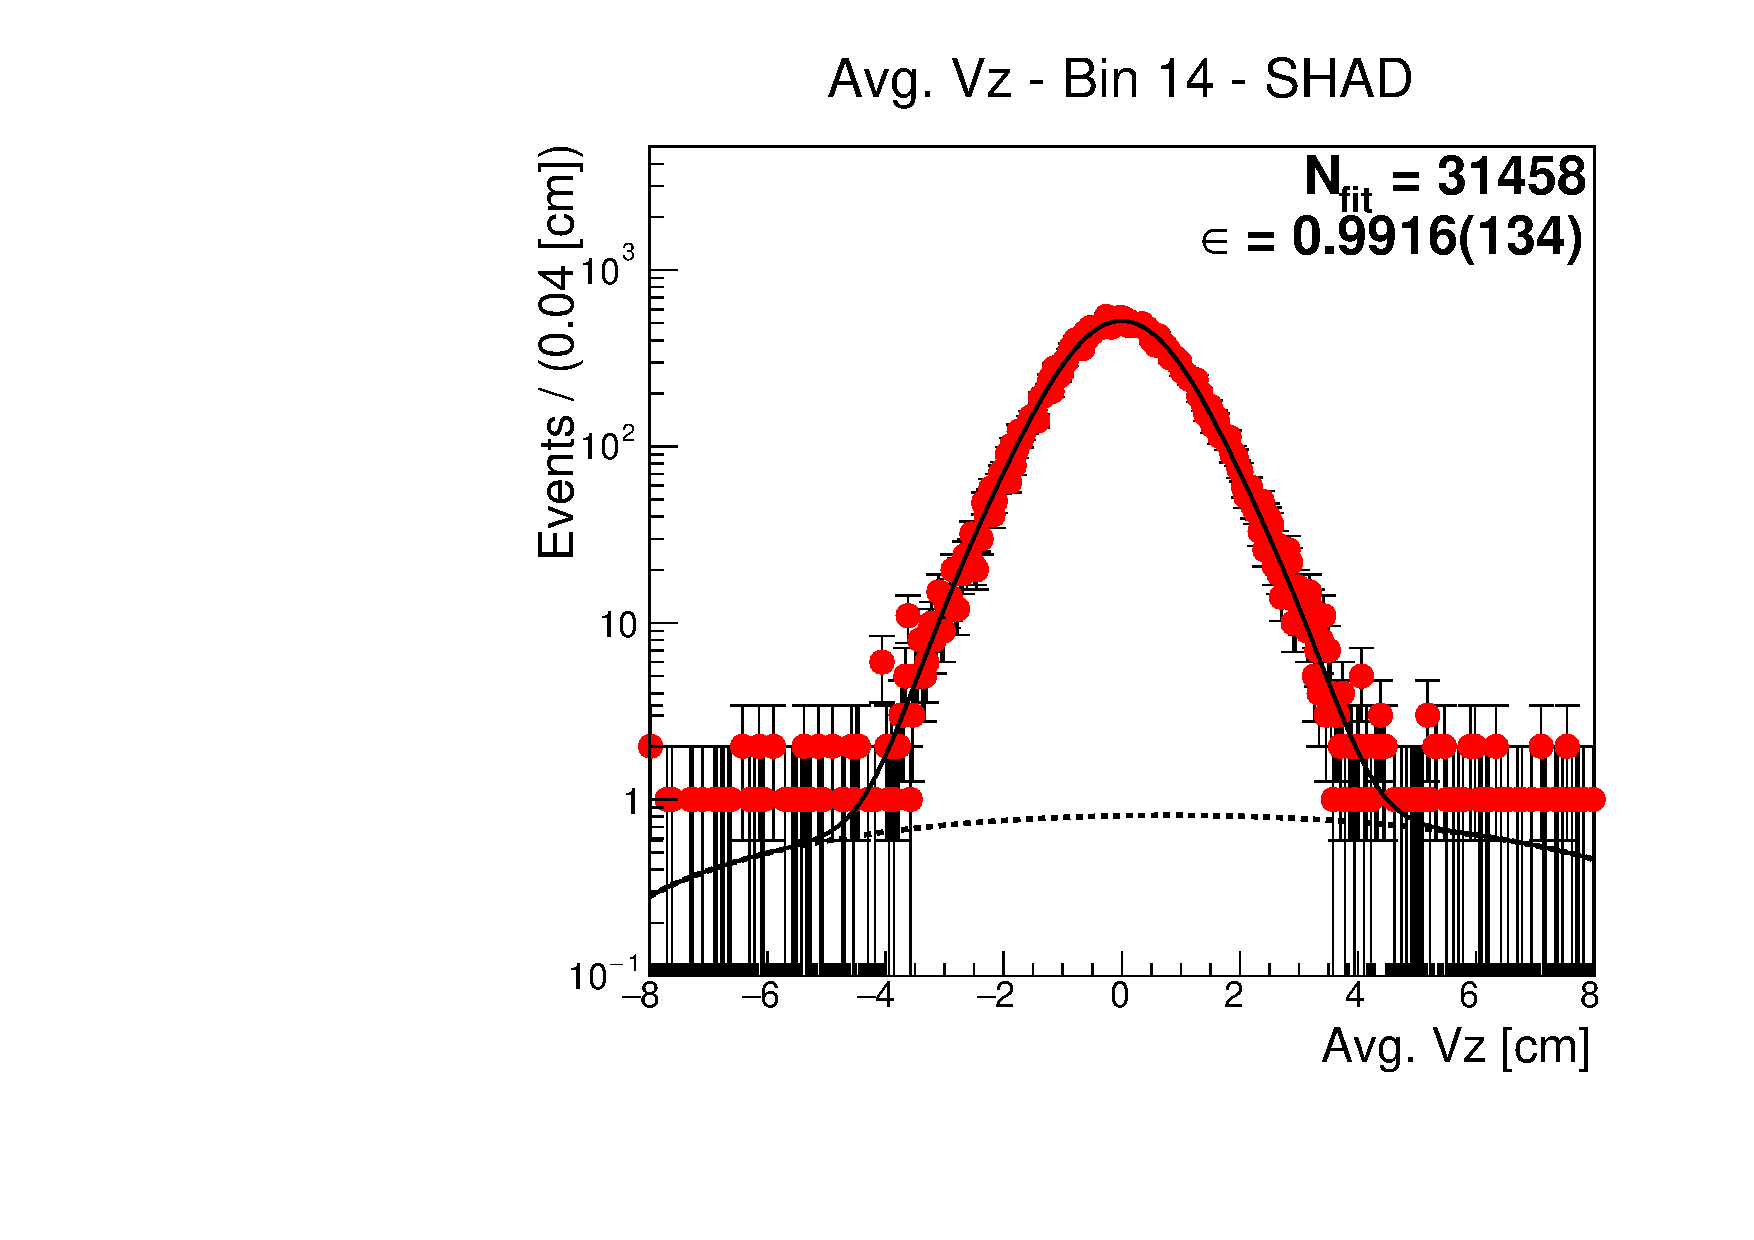
\includegraphics[scale=0.25]{figures/plots/nonDDbar_fit_results/scan/fit_scan_14_data_SHAD.pdf}
\hspace{-0.5cm}
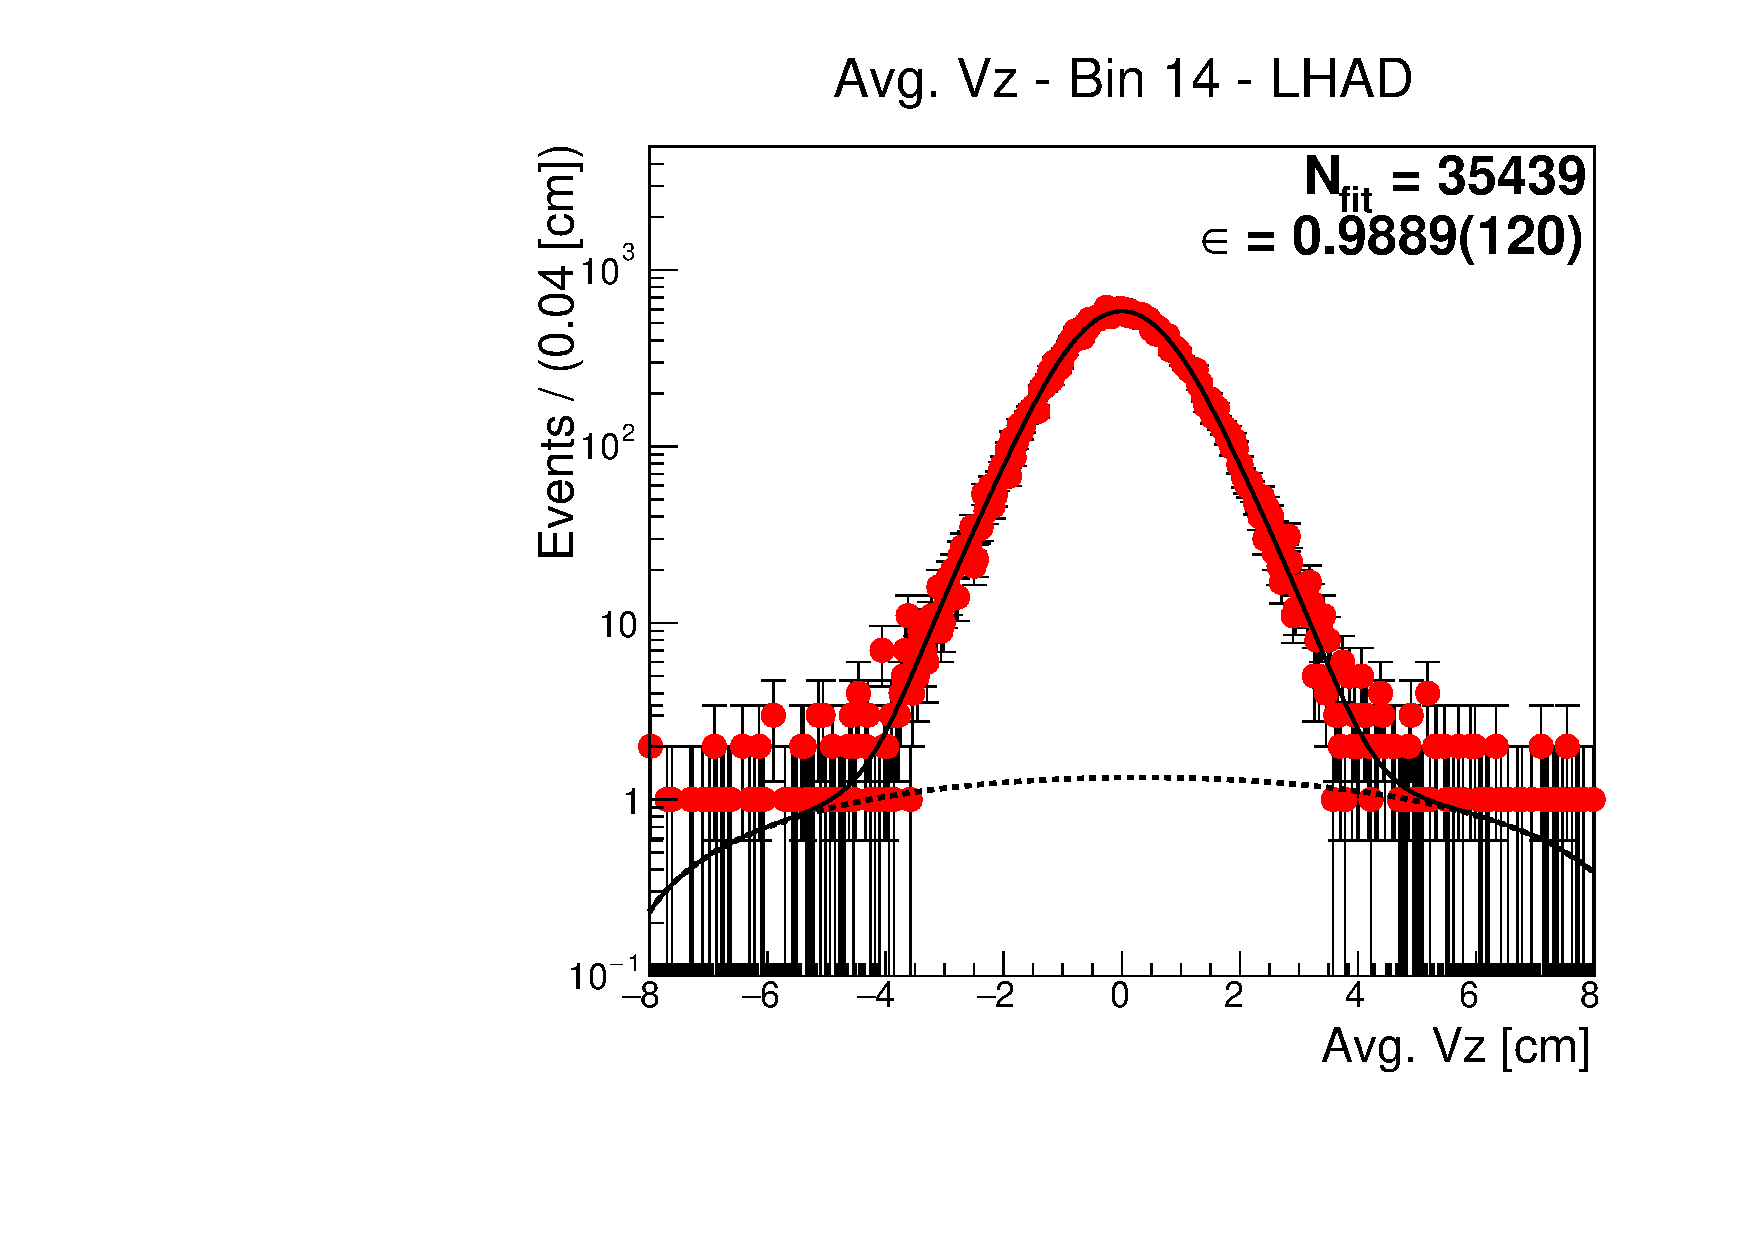
\includegraphics[scale=0.25]{figures/plots/nonDDbar_fit_results/scan/fit_scan_14_data_LHAD.pdf}
\hspace{-0.5cm}
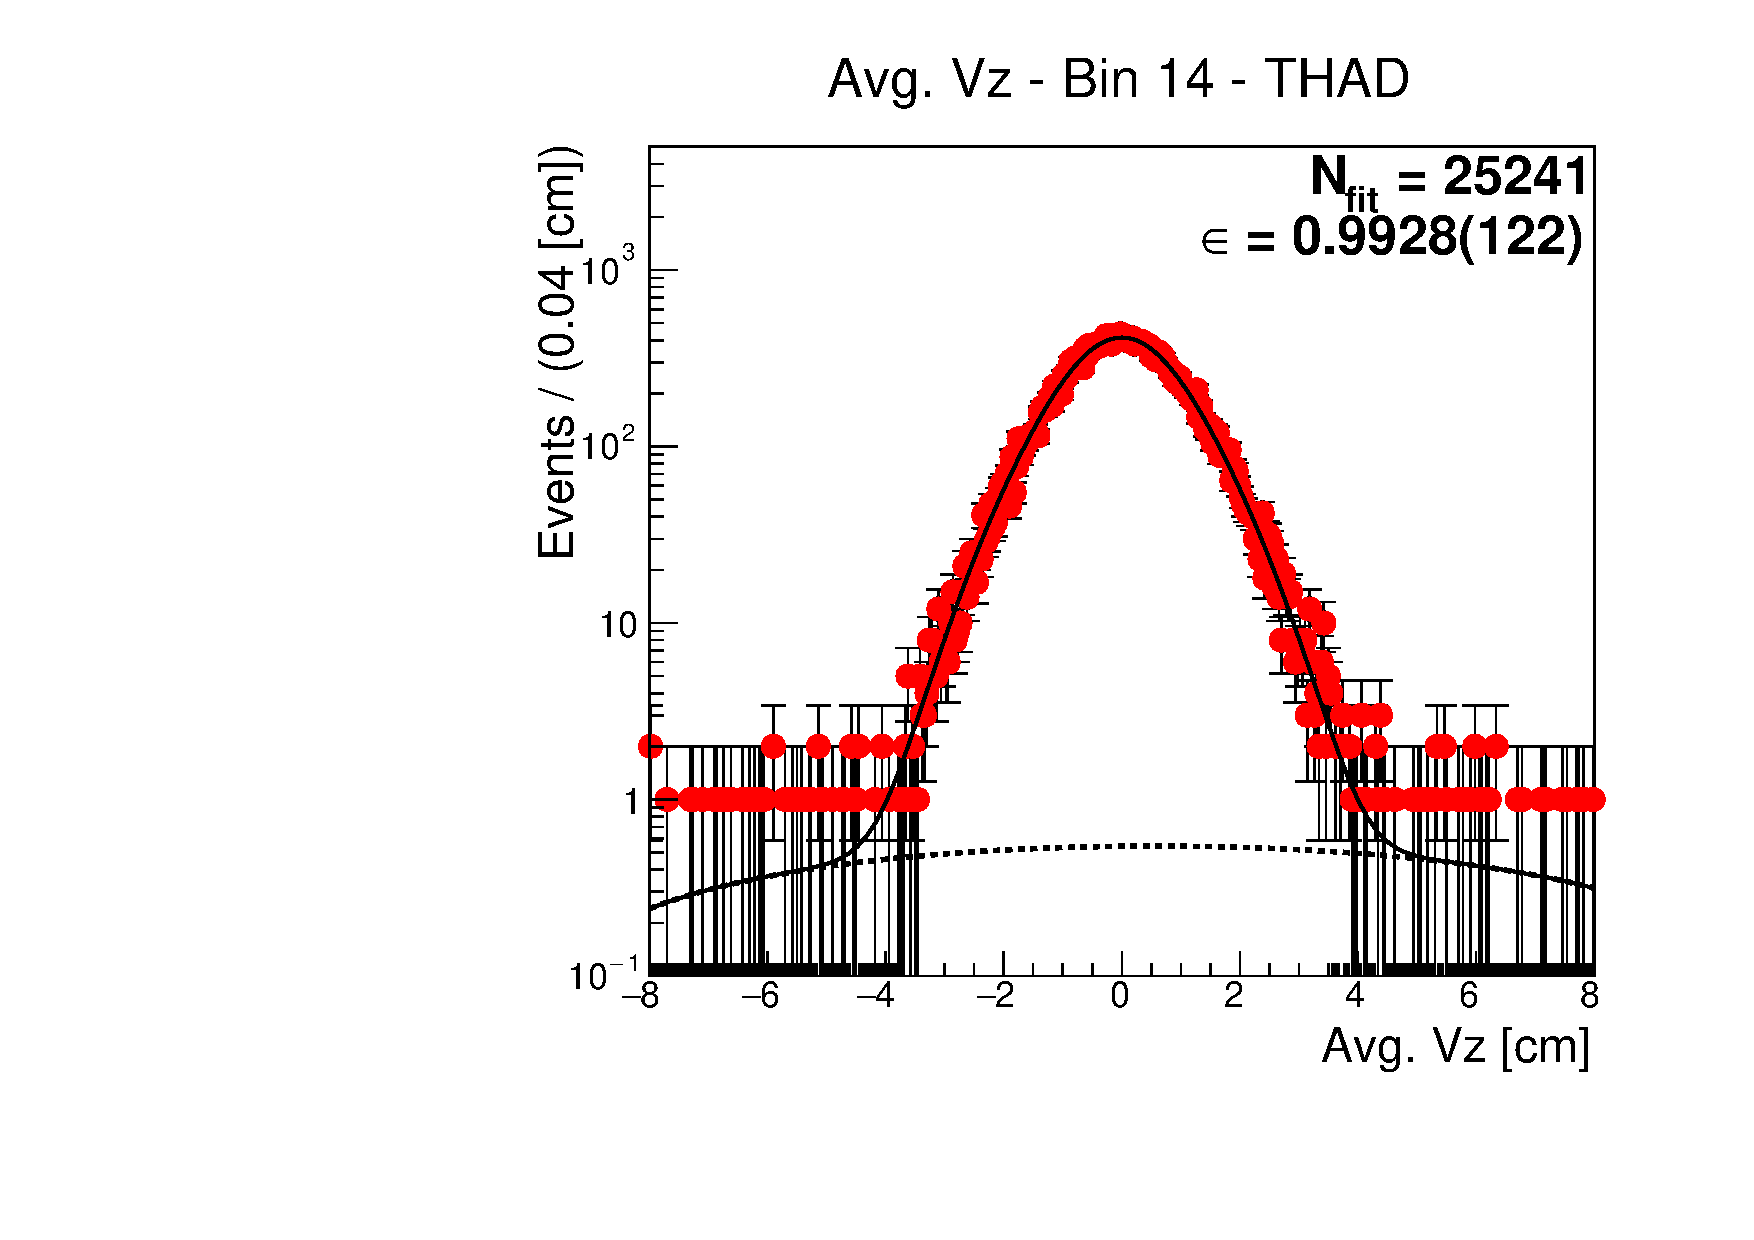
\includegraphics[scale=0.25]{figures/plots/nonDDbar_fit_results/scan/fit_scan_14_data_THAD.pdf}
\caption{Fits to determine the number of hadrons in the 3774 (Scan) data sample.}
{This includes results for SHAD (left), LHAD (middle), and THAD (right).}
\label{fig:hadron_fits_scan_14}
\end{figure}

\begin{figure}[H]
\centering
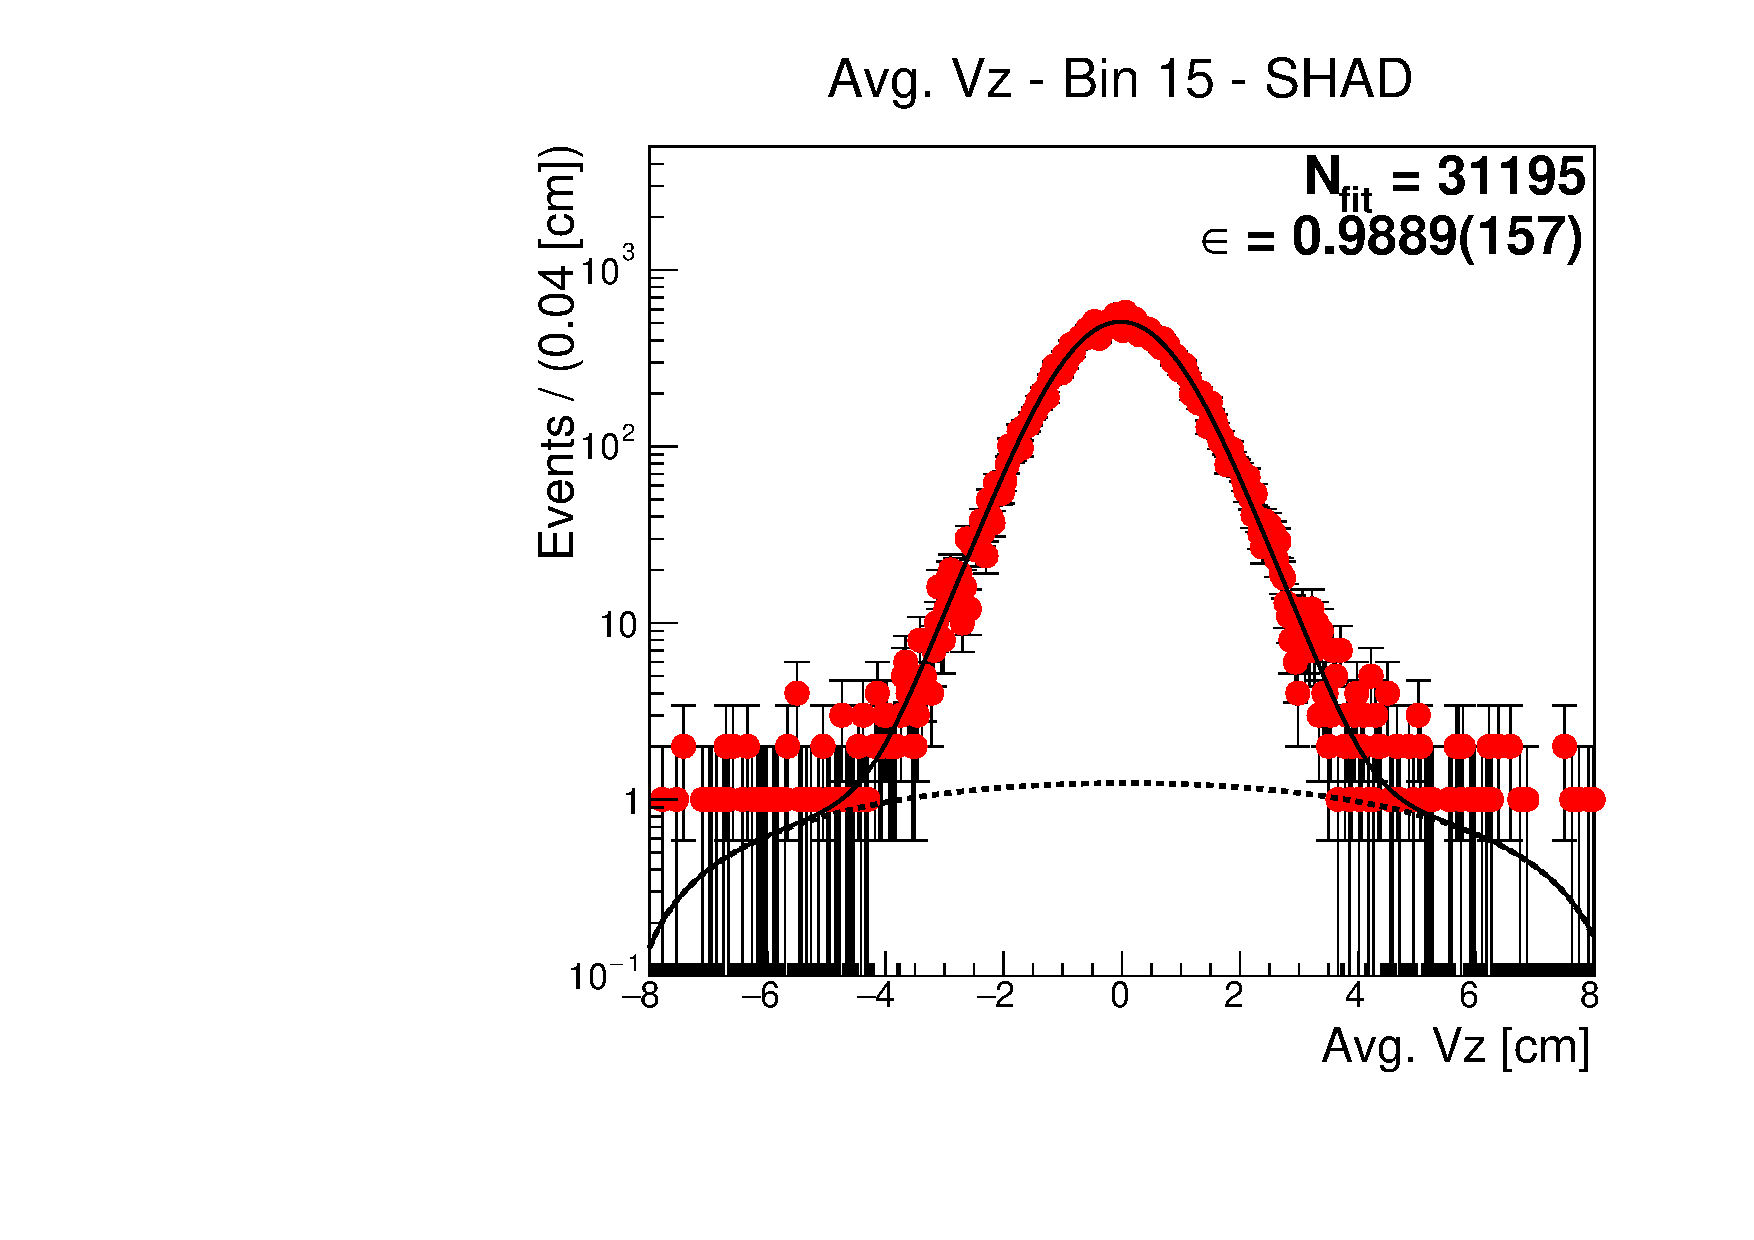
\includegraphics[scale=0.25]{figures/plots/nonDDbar_fit_results/scan/fit_scan_15_data_SHAD.pdf}
\hspace{-0.5cm}
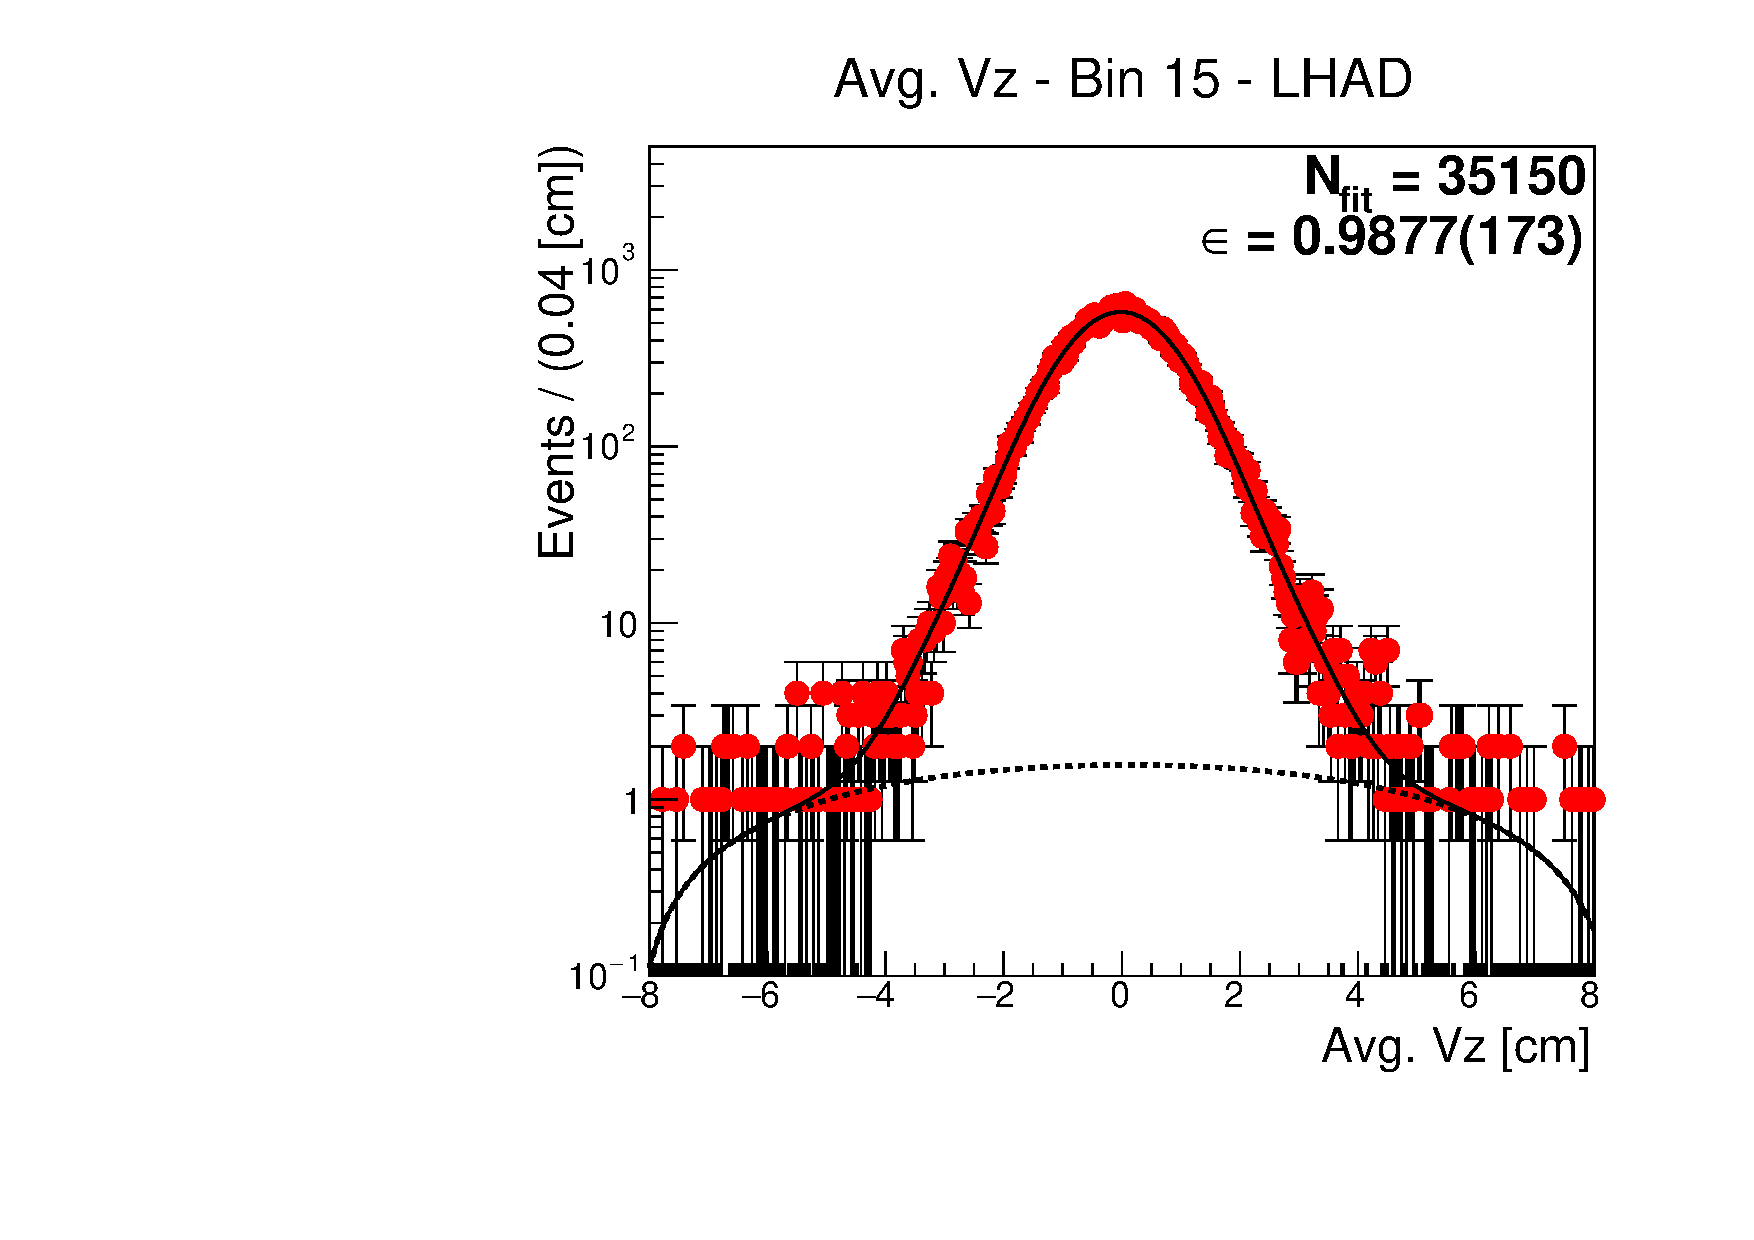
\includegraphics[scale=0.25]{figures/plots/nonDDbar_fit_results/scan/fit_scan_15_data_LHAD.pdf}
\hspace{-0.5cm}
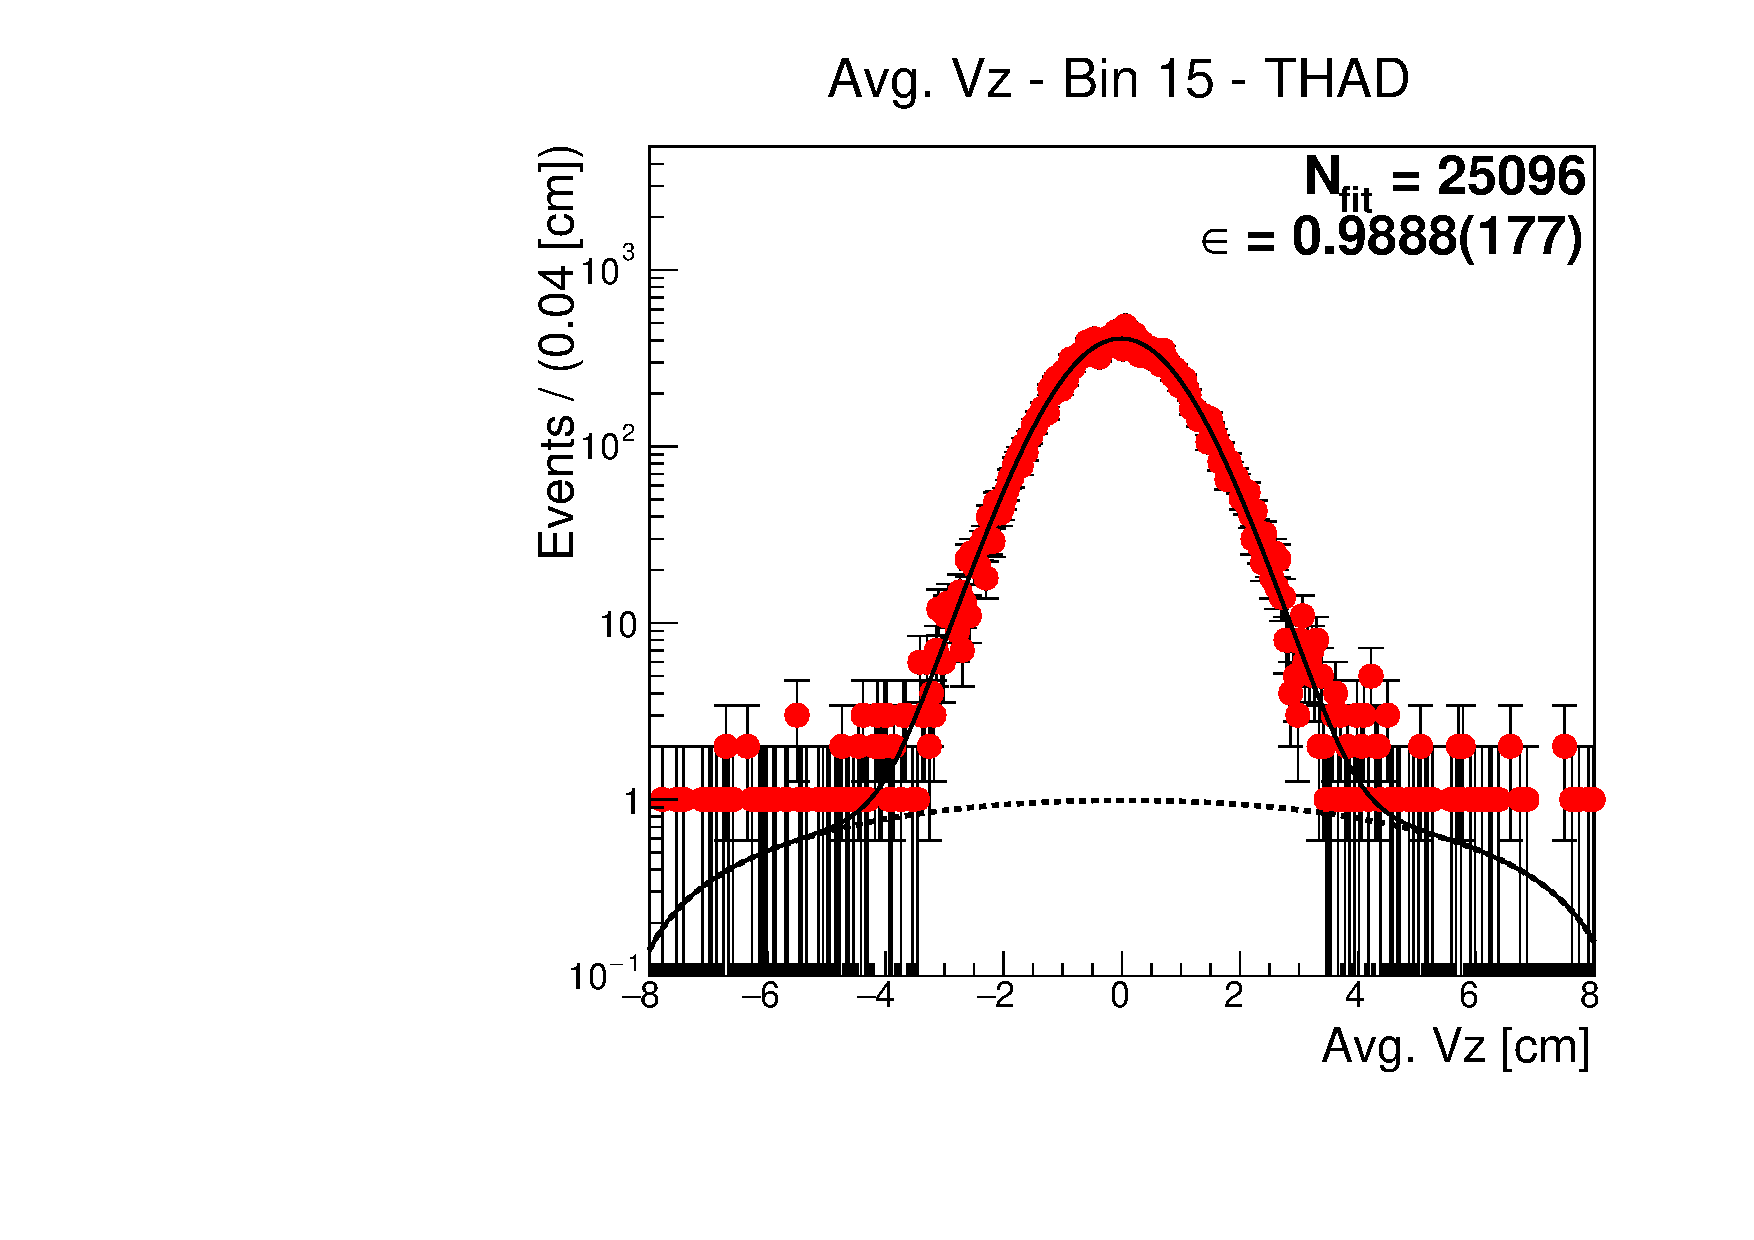
\includegraphics[scale=0.25]{figures/plots/nonDDbar_fit_results/scan/fit_scan_15_data_THAD.pdf}
\caption{Fits to determine the number of hadrons in the 3777 (Scan) data sample.}
{This includes results for SHAD (left), LHAD (middle), and THAD (right).}
\label{fig:hadron_fits_scan_15}
\end{figure}

\begin{figure}[H]
\centering
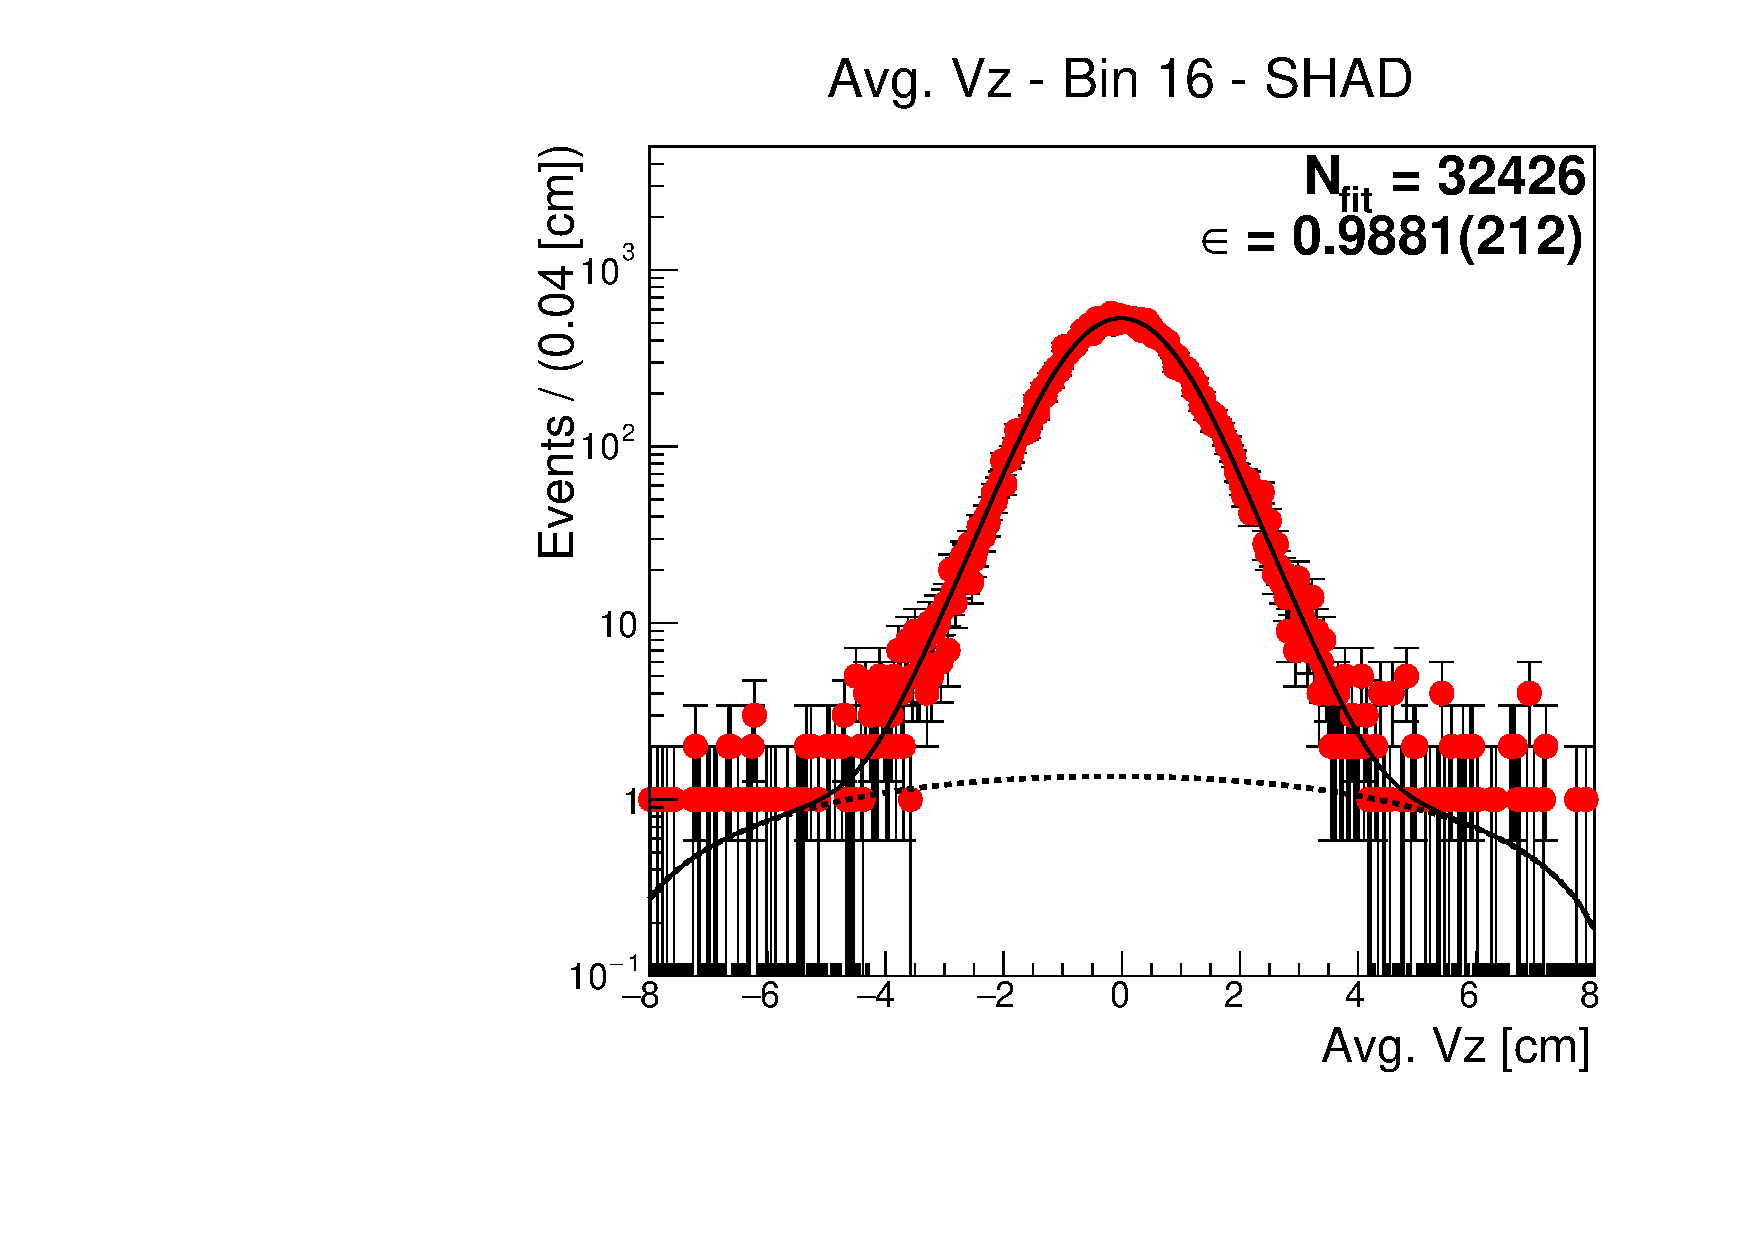
\includegraphics[scale=0.25]{figures/plots/nonDDbar_fit_results/scan/fit_scan_16_data_SHAD.pdf}
\hspace{-0.5cm}
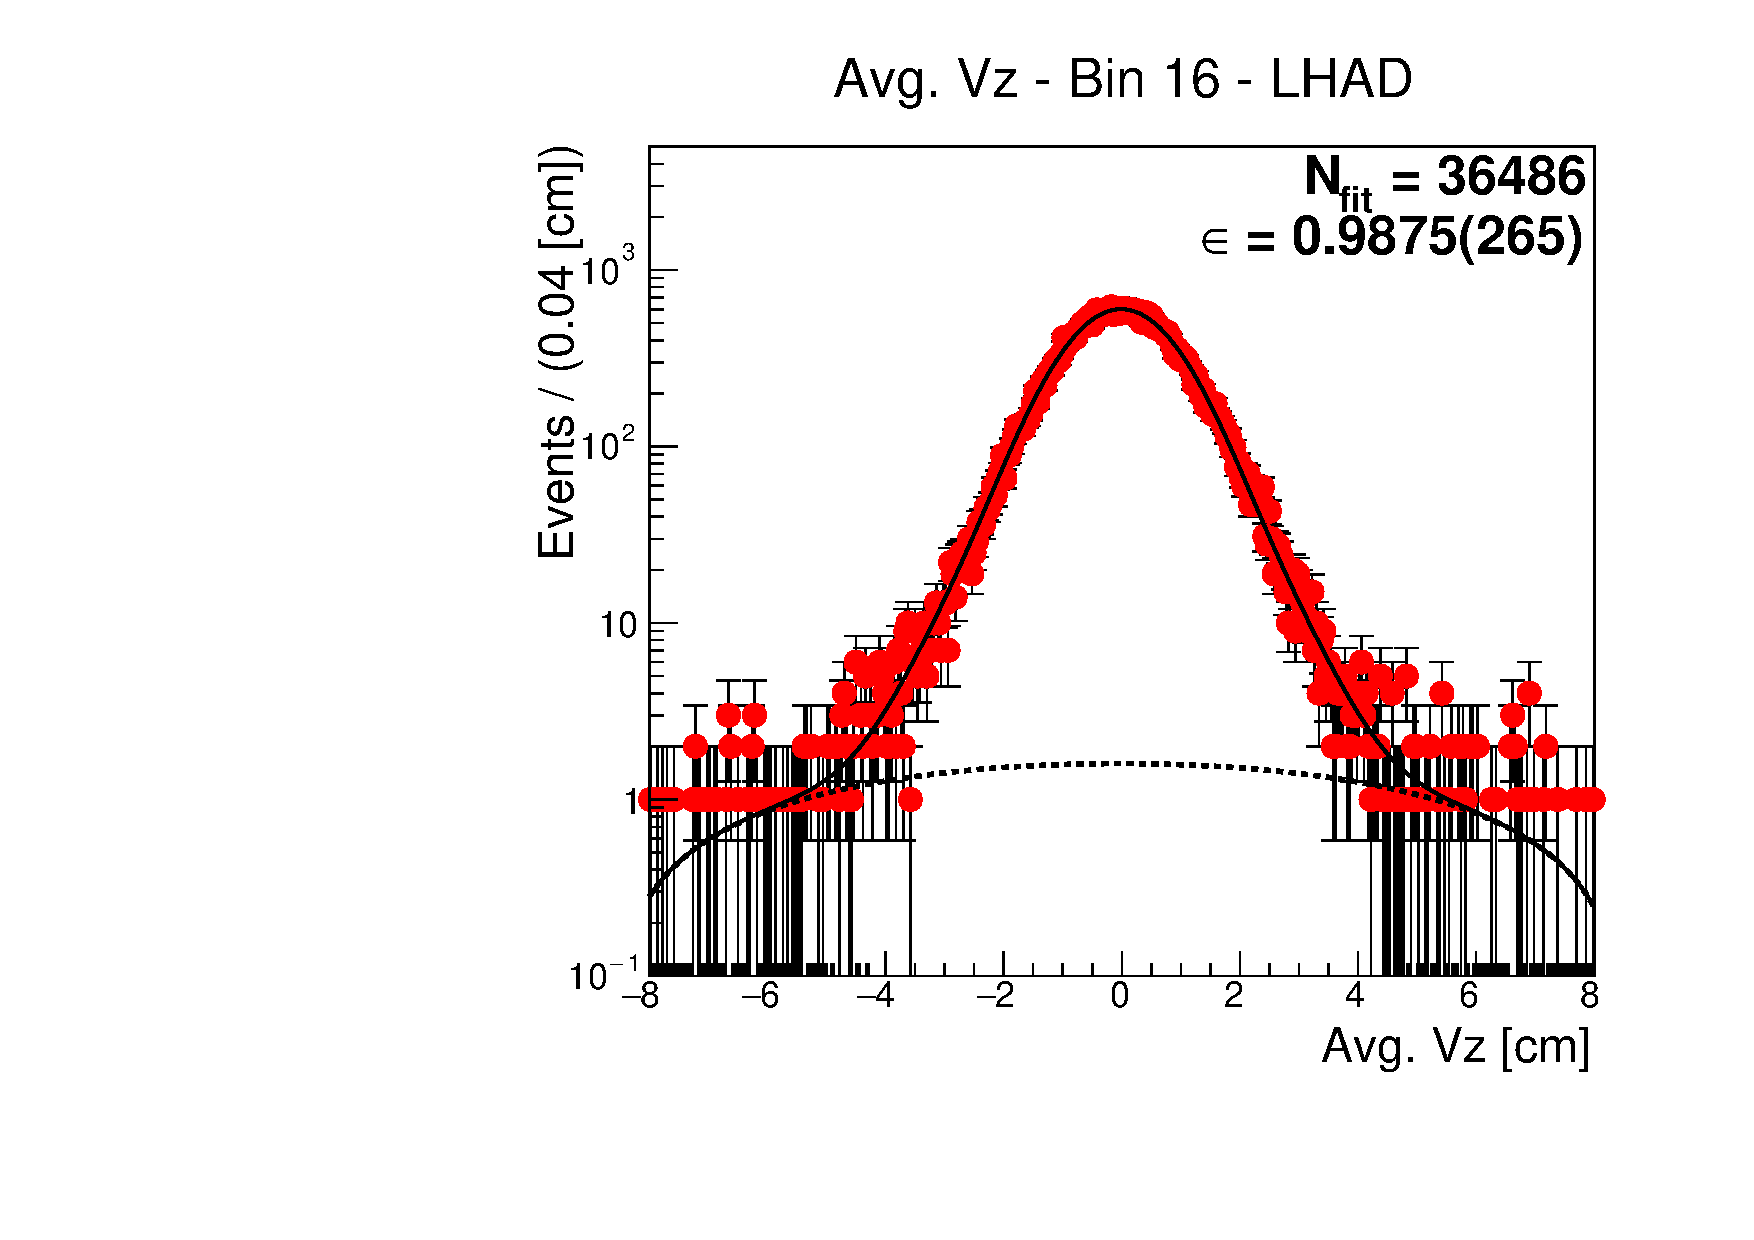
\includegraphics[scale=0.25]{figures/plots/nonDDbar_fit_results/scan/fit_scan_16_data_LHAD.pdf}
\hspace{-0.5cm}
\includegraphics[scale=0.25]{figures/plots/nonDDbar_fit_results/scan/fit_scan_16_data_THAD.pdf}
\caption{Fits to determine the number of hadrons in the 3780 (Scan) data sample.}
{This includes results for SHAD (left), LHAD (middle), and THAD (right).}
\label{fig:hadron_fits_scan_16}
\end{figure}

\begin{figure}[H]
\centering
\includegraphics[scale=0.25]{figures/plots/nonDDbar_fit_results/scan/fit_scan_17_data_SHAD.pdf}
\hspace{-0.5cm}
\includegraphics[scale=0.25]{figures/plots/nonDDbar_fit_results/scan/fit_scan_17_data_LHAD.pdf}
\hspace{-0.5cm}
\includegraphics[scale=0.25]{figures/plots/nonDDbar_fit_results/scan/fit_scan_17_data_THAD.pdf}
\caption{Fits to determine the number of hadrons in the 3782 (Scan) data sample.}
{This includes results for SHAD (left), LHAD (middle), and THAD (right).}
\label{fig:hadron_fits_scan_17}
\end{figure}

\begin{figure}[H]
\centering
\includegraphics[scale=0.25]{figures/plots/nonDDbar_fit_results/scan/fit_scan_18_data_SHAD.pdf}
\hspace{-0.5cm}
\includegraphics[scale=0.25]{figures/plots/nonDDbar_fit_results/scan/fit_scan_18_data_LHAD.pdf}
\hspace{-0.5cm}
\includegraphics[scale=0.25]{figures/plots/nonDDbar_fit_results/scan/fit_scan_18_data_THAD.pdf}
\caption{Fits to determine the number of hadrons in the 3786 (Scan) data sample.}
{This includes results for SHAD (left), LHAD (middle), and THAD (right).}
\label{fig:hadron_fits_scan_18}
\end{figure}

\begin{figure}[H]
\centering
\includegraphics[scale=0.25]{figures/plots/nonDDbar_fit_results/scan/fit_scan_19_data_SHAD.pdf}
\hspace{-0.5cm}
\includegraphics[scale=0.25]{figures/plots/nonDDbar_fit_results/scan/fit_scan_19_data_LHAD.pdf}
\hspace{-0.5cm}
\includegraphics[scale=0.25]{figures/plots/nonDDbar_fit_results/scan/fit_scan_19_data_THAD.pdf}
\caption{Fits to determine the number of hadrons in the 3789 (Scan) data sample.}
{This includes results for SHAD (left), LHAD (middle), and THAD (right).}
\label{fig:hadron_fits_scan_19}
\end{figure}

\begin{figure}[H]
\centering
\includegraphics[scale=0.25]{figures/plots/nonDDbar_fit_results/scan/fit_scan_20_data_SHAD.pdf}
\hspace{-0.5cm}
\includegraphics[scale=0.25]{figures/plots/nonDDbar_fit_results/scan/fit_scan_20_data_LHAD.pdf}
\hspace{-0.5cm}
\includegraphics[scale=0.25]{figures/plots/nonDDbar_fit_results/scan/fit_scan_20_data_THAD.pdf}
\caption{Fits to determine the number of hadrons in the 3792 (Scan) data sample.}
{This includes results for SHAD (left), LHAD (middle), and THAD (right).}
\label{fig:hadron_fits_scan_20}
\end{figure}

\begin{figure}[H]
\centering
\includegraphics[scale=0.25]{figures/plots/nonDDbar_fit_results/scan/fit_scan_21_data_SHAD.pdf}
\hspace{-0.5cm}
\includegraphics[scale=0.25]{figures/plots/nonDDbar_fit_results/scan/fit_scan_21_data_LHAD.pdf}
\hspace{-0.5cm}
\includegraphics[scale=0.25]{figures/plots/nonDDbar_fit_results/scan/fit_scan_21_data_THAD.pdf}
\caption{Fits to determine the number of hadrons in the 3797 (Scan) data sample.}
{This includes results for SHAD (left), LHAD (middle), and THAD (right).}
\label{fig:hadron_fits_scan_21}
\end{figure}

\begin{figure}[H]
\centering
\includegraphics[scale=0.25]{figures/plots/nonDDbar_fit_results/scan/fit_scan_22_data_SHAD.pdf}
\hspace{-0.5cm}
\includegraphics[scale=0.25]{figures/plots/nonDDbar_fit_results/scan/fit_scan_22_data_LHAD.pdf}
\hspace{-0.5cm}
\includegraphics[scale=0.25]{figures/plots/nonDDbar_fit_results/scan/fit_scan_22_data_THAD.pdf}
\caption{Fits to determine the number of hadrons in the 3800 (Scan) data sample.}
{This includes results for SHAD (left), LHAD (middle), and THAD (right).}
\label{fig:hadron_fits_scan_22}
\end{figure}

\begin{figure}[H]
\centering
\includegraphics[scale=0.25]{figures/plots/nonDDbar_fit_results/scan/fit_scan_23_data_SHAD.pdf}
\hspace{-0.5cm}
\includegraphics[scale=0.25]{figures/plots/nonDDbar_fit_results/scan/fit_scan_23_data_LHAD.pdf}
\hspace{-0.5cm}
\includegraphics[scale=0.25]{figures/plots/nonDDbar_fit_results/scan/fit_scan_23_data_THAD.pdf}
\caption{Fits to determine the number of hadrons in the 3802 (Scan) data sample.}
{This includes results for SHAD (left), LHAD (middle), and THAD (right).}
\label{fig:hadron_fits_scan_23}
\end{figure}

\begin{figure}[H]
\centering
\includegraphics[scale=0.25]{figures/plots/nonDDbar_fit_results/scan/fit_scan_24_data_SHAD.pdf}
\hspace{-0.5cm}
\includegraphics[scale=0.25]{figures/plots/nonDDbar_fit_results/scan/fit_scan_24_data_LHAD.pdf}
\hspace{-0.5cm}
\includegraphics[scale=0.25]{figures/plots/nonDDbar_fit_results/scan/fit_scan_24_data_THAD.pdf}
\caption{Fits to determine the number of hadrons in the 3807 (Scan) data sample.}
{This includes results for SHAD (left), LHAD (middle), and THAD (right).}
\label{fig:hadron_fits_scan_24}
\end{figure}

\begin{figure}[H]
\centering
\includegraphics[scale=0.25]{figures/plots/nonDDbar_fit_results/scan/fit_scan_25_data_SHAD.pdf}
\hspace{-0.5cm}
\includegraphics[scale=0.25]{figures/plots/nonDDbar_fit_results/scan/fit_scan_25_data_LHAD.pdf}
\hspace{-0.5cm}
\includegraphics[scale=0.25]{figures/plots/nonDDbar_fit_results/scan/fit_scan_25_data_THAD.pdf}
\caption{Fits to determine the number of hadrons in the 3809 (Scan) data sample.}
{This includes results for SHAD (left), LHAD (middle), and THAD (right).}
\label{fig:hadron_fits_scan_25}
\end{figure}

\begin{figure}[H]
\centering
\includegraphics[scale=0.25]{figures/plots/nonDDbar_fit_results/scan/fit_scan_26_data_SHAD.pdf}
\hspace{-0.5cm}
\includegraphics[scale=0.25]{figures/plots/nonDDbar_fit_results/scan/fit_scan_26_data_LHAD.pdf}
\hspace{-0.5cm}
\includegraphics[scale=0.25]{figures/plots/nonDDbar_fit_results/scan/fit_scan_26_data_THAD.pdf}
\caption{Fits to determine the number of hadrons in the 3813 (Scan) data sample.}
{This includes results for SHAD (left), LHAD (middle), and THAD (right).}
\label{fig:hadron_fits_scan_26}
\end{figure}

\begin{figure}[H]
\centering
\includegraphics[scale=0.25]{figures/plots/nonDDbar_fit_results/scan/fit_scan_27_data_SHAD.pdf}
\hspace{-0.5cm}
\includegraphics[scale=0.25]{figures/plots/nonDDbar_fit_results/scan/fit_scan_27_data_LHAD.pdf}
\hspace{-0.5cm}
\includegraphics[scale=0.25]{figures/plots/nonDDbar_fit_results/scan/fit_scan_27_data_THAD.pdf}
\caption{Fits to determine the number of hadrons in the 3815 (Scan) data sample.}
{This includes results for SHAD (left), LHAD (middle), and THAD (right).}
\label{fig:hadron_fits_scan_27}
\end{figure}

\begin{figure}[H]
\centering
\includegraphics[scale=0.25]{figures/plots/nonDDbar_fit_results/scan/fit_scan_28_data_SHAD.pdf}
\hspace{-0.5cm}
\includegraphics[scale=0.25]{figures/plots/nonDDbar_fit_results/scan/fit_scan_28_data_LHAD.pdf}
\hspace{-0.5cm}
\includegraphics[scale=0.25]{figures/plots/nonDDbar_fit_results/scan/fit_scan_28_data_THAD.pdf}
\caption{Fits to determine the number of hadrons in the 3822 (Scan) data sample.}
{This includes results for SHAD (left), LHAD (middle), and THAD (right).}
\label{fig:hadron_fits_scan_28}
\end{figure}

\begin{figure}[H]
\centering
\includegraphics[scale=0.25]{figures/plots/nonDDbar_fit_results/scan/fit_scan_29_data_SHAD.pdf}
\hspace{-0.5cm}
\includegraphics[scale=0.25]{figures/plots/nonDDbar_fit_results/scan/fit_scan_29_data_LHAD.pdf}
\hspace{-0.5cm}
\includegraphics[scale=0.25]{figures/plots/nonDDbar_fit_results/scan/fit_scan_29_data_THAD.pdf}
\caption{Fits to determine the number of hadrons in the 3832 (Scan) data sample.}
{This includes results for SHAD (left), LHAD (middle), and THAD (right).}
\label{fig:hadron_fits_scan_29}
\end{figure}

\begin{figure}[H]
\centering
\includegraphics[scale=0.25]{figures/plots/nonDDbar_fit_results/scan/fit_scan_30_data_SHAD.pdf}
\hspace{-0.5cm}
\includegraphics[scale=0.25]{figures/plots/nonDDbar_fit_results/scan/fit_scan_30_data_LHAD.pdf}
\hspace{-0.5cm}
\includegraphics[scale=0.25]{figures/plots/nonDDbar_fit_results/scan/fit_scan_30_data_THAD.pdf}
\caption{Fits to determine the number of hadrons in the 3839 (Scan) data sample.}
{This includes results for SHAD (left), LHAD (middle), and THAD (right).}
\label{fig:hadron_fits_scan_30}
\end{figure}

\begin{figure}[H]
\centering
\includegraphics[scale=0.25]{figures/plots/nonDDbar_fit_results/scan/fit_scan_31_data_SHAD.pdf}
\hspace{-0.5cm}
\includegraphics[scale=0.25]{figures/plots/nonDDbar_fit_results/scan/fit_scan_31_data_LHAD.pdf}
\hspace{-0.5cm}
\includegraphics[scale=0.25]{figures/plots/nonDDbar_fit_results/scan/fit_scan_31_data_THAD.pdf}
\caption{Fits to determine the number of hadrons in the 3849 (Scan) data sample.}
{This includes results for SHAD (left), LHAD (middle), and THAD (right).}
\label{fig:hadron_fits_scan_31}
\end{figure}

\begin{figure}[H]
\centering
\includegraphics[scale=0.25]{figures/plots/nonDDbar_fit_results/scan/fit_scan_32_data_SHAD.pdf}
\hspace{-0.5cm}
\includegraphics[scale=0.25]{figures/plots/nonDDbar_fit_results/scan/fit_scan_32_data_LHAD.pdf}
\hspace{-0.5cm}
\includegraphics[scale=0.25]{figures/plots/nonDDbar_fit_results/scan/fit_scan_32_data_THAD.pdf}
\caption{Fits to determine the number of hadrons in the 3855 (Scan) data sample.}
{This includes results for SHAD (left), LHAD (middle), and THAD (right).}
\label{fig:hadron_fits_scan_32}
\end{figure}

\begin{figure}[H]
\centering
\includegraphics[scale=0.25]{figures/plots/nonDDbar_fit_results/scan/fit_scan_33_data_SHAD.pdf}
\hspace{-0.5cm}
\includegraphics[scale=0.25]{figures/plots/nonDDbar_fit_results/scan/fit_scan_33_data_LHAD.pdf}
\hspace{-0.5cm}
\includegraphics[scale=0.25]{figures/plots/nonDDbar_fit_results/scan/fit_scan_33_data_THAD.pdf}
\caption{Fits to determine the number of hadrons in the 3863 (Scan) data sample.}
{This includes results for SHAD (left), LHAD (middle), and THAD (right).}
\label{fig:hadron_fits_scan_33}
\end{figure}
